\documentclass{article}

\usepackage{amsmath,geometry,graphicx,array,makecell,enumitem,bm,booktabs,multirow,pgfplots,bm,amssymb,mathtools,xcolor,nicematrix,float}
\usepackage[amsmath]{ntheorem}
\usepackage[hidelinks,naturalnames]{hyperref}
\usepackage[nameinlink,noabbrev]{cleveref}
\usepackage{fancyhdr}
\pagestyle{fancy}
\fancyhead[L]{\itshape\nouppercase{\leftmark}}
\fancyhead[R]{B8 Symmetry}


\title{Symmetry}
\author{Yue Wu}

\geometry{a4paper,hmargin=1.1in,vmargin=1.2in}

\setlength{\parskip}{1em}
\tolerance=1000
\emergencystretch=1em
\hyphenpenalty=1000
\exhyphenpenalty=100
\righthyphenmin=3

\theoremstyle{plain}\theoremheaderfont{\normalfont\itshape}\theorembodyfont{\rmfamily}\theoremseparator{.}\newtheorem*{rem}{Remark}\newtheorem*{ex}{Example}\newtheorem*{proof}{Proof}\newtheorem*{altp}{Alternative proof}

\theoremstyle{plain}\theoremheaderfont{\normalfont\bfseries}\theorembodyfont{\rmfamily}\theoremseparator{.}\newtheorem{thm}{Theorem}[section]\newtheorem{lem}[thm]{Lemma}\newtheorem{prop}[thm]{Proposition}\newtheorem*{cor}{Corollary}\newtheorem{defn}[thm]{Definition}\newtheorem{clm}[thm]{Claim}\newtheorem{clminproof}{Claim}\newtheorem*{law}{Law}\newtheorem{pos}[thm]{Postulate}

\theoremstyle{break}\theoremheaderfont{\normalfont\itshape}\theorembodyfont{\rmfamily}\theoremseparator{.\medskip}\newtheorem*{proofskip}{Proof}\newtheorem*{exs}{Examples}\newtheorem*{rems}{Remarks}

\theoremstyle{break}\theoremheaderfont{\normalfont\bfseries}\theorembodyfont{\rmfamily}\theoremseparator{.\medskip}\newtheorem{lemskip}[thm]{Lemma}\newtheorem{defnskip}[thm]{Definition}\newtheorem{propskip}[thm]{Proposition}\newtheorem{thmskip}[thm]{Theorem}

\crefname{thm}{Theorem}{Theorems}\crefname{defn}{Definition}{Definitions}\crefname{lem}{Lemma}{Lemmas}\crefname{lemskip}{Lemma}{Lemmas}\crefname{cor}{Corollary}{Corollaries} \crefname{prop}{Proposition}{Propositions}\crefname{clm}{Claim}{Claims}\crefname{pos}{Postulate}{Postulates}

\setcounter{tocdepth}{2}
\numberwithin{equation}{section}
\counterwithin{figure}{section}

\NiceMatrixOptions{cell-space-limits = 2pt}

\usetikzlibrary{calc}

\newcommand{\qed}{\hfill\ensuremath{\Box}}
\newcommand{\unit}[1]{\ \mathrm{#1}}
\newcommand{\ii}{\mathrm{i}}
\newcommand{\ee}{\mathrm{e}}
\newcommand{\tp}{^\mathrm{T}}
\newcommand{\dbar}{\mathrm{d}\hspace*{-0.14em}\bar{}\hspace*{0.12em}}
\newcommand{\dd}[2][]{\mathrm{d}^{#1} #2\,}
\renewcommand{\d}[2][]{\mathrm{d}^{#1} #2}
\newcommand{\dv}[3][]{\frac{\mathrm{d}^{#1} #2}{{\mathrm{d} #3}^{#1}}}
\newcommand{\pdv}[3][]{\frac{\partial^{#1} #2}{{\partial #3}^{#1}}}
\newcommand{\bra}[1]{\left\langle #1 \right|}
\newcommand{\ket}[1]{\left| #1 \right\rangle}
\newcommand{\braket}[2]{\left\langle #1 \middle| #2 \right\rangle}
\newcommand{\eval}[1]{\left\langle #1 \right\rangle}
\newcommand{\mel}[3]{\left\langle #1 \middle| #2 \middle| #3 \right\rangle}
\newcommand{\expval}[2]{\left\langle #2 \middle| #1 \middle| #2 \right\rangle}
\newcommand{\vb}[1]{\bm{\mathrm{#1}}}
\newcommand{\vu}[1]{\hat{\bm{\mathrm{#1}}}}
\newcommand{\vdot}{\,\bm{\mathrm{\cdot}}\,}
\newcommand{\cross}{\bm{\mathrm{\times}}}
\newcommand{\abs}[1]{\left| #1 \right|}
\newcommand{\norm}[1]{\left\| #1 \right\|}
\newcommand{\grad}{\vb{\nabla}}
\renewcommand{\div}{\vb{\nabla}\cdot}
\newcommand{\curl}{\vb{\nabla}\times}
\newcommand{\laplacian}{\nabla^2}
\newcommand{\RR}{\mathbb{R}}
\newcommand{\CC}{\mathbb{C}}
\newcommand{\DD}{\mathsf{D}}
\newcommand{\II}{\mathsf{I}}
\newcommand{\TT}{\mathsf{T}}
\newcommand{\GL}{\mathrm{GL}}
\newcommand{\SO}{\mathrm{SO}}
\newcommand{\U}{\mathrm{U}}
\DeclareMathOperator{\spn}{span}
\DeclareMathOperator{\Hom}{Hom}
\DeclareMathOperator{\tr}{tr}
\renewcommand{\Re}{\operatorname{Re}}
\renewcommand{\Im}{\operatorname{Im}}

\pgfplotsset{compat=1.18}

\begin{document}
    \setlength{\parindent}{0pt}
	\Huge\textsf{\textbf{Symmetry}}
		
	\Large\textsf{\textbf{University of Cambridge Part II Natural Sciences Tripos}}

	\noindent\makebox[\linewidth]{\rule{\textwidth}{2pt}}

	\large\textsf{\textbf{Yue Wu}}
	\begin{itemize}[topsep=0pt,leftmargin=15pt]
		\item[] \textit{Yusuf Hamied Department of Chemistry\\
		Lensfield Road,\\
		Cambridge, CB2 1EW}\\

		\textit{yw628@cam.ac.uk}
	\end{itemize}
    \thispagestyle{empty}
    \pagenumbering{roman}
    \setlength{\parindent}{15pt}

    \newpage
    \begin{center}
		\textbf{\Large{Acknowledgements}}
	\end{center}
	\large
	Nothing in these lecture notes is original. They are largely based on the notes by Prof. Ali Alavi, who lectured this course in 2024. They are nowhere near accurate representations of what was actually lectured, and in particular, all errors are almost surely mine.

    \vskip 30pt

    \begin{center}
		\textbf{\Large{Preface}}
	\end{center}
	\large
    This course focuses on the foundational level of group theory and representation theory in the context of chemistry and molecular symmetry. If you want a more mathematical (and hence more abstract) treatment on basic groups and representations, you can look at my notes on Natural Sciences Tripos Part IB \textit{Mathematical Methods}. This level of knowledge is essential (and should be enough) for a good grasp on theoretical chemistry. Slightly more advanced notes on groups (and rings and modules) can be found in Mathematical Tripos Part IB \textit{Groups, Rings and Modules}, but they are largely irrelevant to chemistry.

    \normalsize
    \newpage
	\tableofcontents
	\newpage
    \pagenumbering{arabic}

    \section{Symmetry}
    \begin{defn}
        For a system with Hamiltonian \(\hat{H}\), a \textit{symmetry operator} is an operator \(\hat{R}\) such that the inverse \(\hat{R}^{-1}\) exists and commutes with the Hamiltonian
        \begin{equation}
            \hat{R}\hat{H}=\hat{H}\hat{R}\,.
        \end{equation}
    \end{defn}
    The above condition can be trivially rewritten as
    \begin{equation}
        \hat{H}=\hat{R}\hat{H}\hat{R}^{-1}\quad\text{or}\quad\hat{H}=\hat{R}^{-1}\hat{H}\hat{R}\,.
    \end{equation}
    Then if we have \(\ket{\psi}\) an eigenstate of the Hamiltonian
    \begin{equation}
        \hat{H}\ket{\psi}=E\ket{\psi}\,,
    \end{equation}
    \(\hat{R}\ket{\psi}\) is also an eigenstate of \(\hat{H}\) with the same eigenvalue.
    \begin{equation}
        \hat{H}\hat{R}\ket{\psi}=\hat{R}\hat{H}\ket{\psi}=\hat{R}E\ket{\psi}=E\hat{R}\ket{\psi}\,.
    \end{equation}
    The resulting state \(\hat{R}\ket{\psi}\) may be physically equivalent to \(\ket{\psi}\), i.e. \(\hat{R}\ket{\psi}=c\ket{\psi}\) for some \(c\in\CC\), but otherwise \(\ket{\psi}\) and \(\hat{R}\ket{\psi}\) are different states with the same eigenvalue. We see that symmetry leads to degeneracy.

    We are going to make a postulate.
    \begin{pos}
        If a set of eigenstates are degenerate, then the degeneracy must be a consequence of some symmetry.
    \end{pos}
    This is to say, we postulate that any degeneracy has an underlying symmetry (possibly hidden), rather than being truly \textit{accidental}.

    \textit{Example.} For a Hydrogen atom, the three \(\mathrm{2p}\) states are degenerate. They are related by spatial rotations of \(90^\circ\). The \(\mathrm{2s}\) is also degenerate with the three \(\mathrm{2p}\) states. In this case there is no geometric symmetry operations that transform e.g. \(\ket{\mathrm{2s}}\) to \(\ket{2p_z}\), but there do exist symmetry operators that transform \(\ket{\mathrm{2s}}\) to \(\ket{2p_z}\) --- it is only that we cannot find a corresponding geometric representation in our physical space.\footnote{Let's have a close look at the Hamiltonian of a hydrogen atom:
    \begin{equation}
        \hat{H}=-\frac{1}{2}\laplacian-\frac{1}{r}=-\frac{1}{2}\left[\frac{1}{r^2}\pdv{}{r}\left(r^2\pdv{}{r}\right)-\frac{\hat{L}^2}{r^2}\right]-\frac{1}{r}\,,
    \end{equation}
    where we have used the atomic units. As we all know, we can label a hydrogen energy eigenstate by \(\ket{n,\ell,m}\). There is no \(\hat{L}_z\) involved in the expression of the Hamiltonian, so we are quite happy to accept that the energy of the hydrogen is independent of \(m\), i.e. the states that differ only by \(m\) are degenerate. This naturally follows from spherical rotational symmetry of hydrogen atom characterised by the \(\SO(3)\) group (see later) --- a hydrogen atom should have no preference on in which direction the angular momentum lies. However, we do have \(\hat{L}^2\) appearing explicitly in the Hamiltonian, so we would not expect states with different \(\ell\)'s to be degenerate. In fact, this is true for any other atom, or indeed for any other central potentials --- the degeneracy is \(2\ell+1\) for the states that differ by \(m_\ell\) only. However, there is another conserved quantity in hydrogen atom that arises because the potential is exactly \(\sim r^{-1}\). It is called the \textit{Runge--Lenz} vector, which also appears in many other places like planetary orbits. This enhances the symmetry group of a hydrogen atom from \(\SO(3)\) to \(\SO(4)\). Roughly speaking, aside from simply rotating our system, we can also trade radial kinetic energy and Coulomb potential for different orbital kinetic energy whilst keeping the total energy constant. This raises the degeneracy of a hydrogen atom from \(2\ell+1\) to \(n^2\).}

    \subsection{Molecular Symmetry}
    We will consider molecular systems for which the Hamiltonian looks like
    \begin{equation}
        \hat{H}=-\sum_{i}\frac{\hbar^2}{2m_i}\laplacian_i+V(\{\vb{r}_i\})
    \end{equation}
    such that the potential term \(V\) only depends on the distances between the particles. Let's see what symmetry such systems can have.

    We can divide symmetries into two types: \textit{continuous symmetry} and \textit{discrete symmetry}. Continuous symmetries are those that can be parameterised by continuous parameters (e.g. rotation is parameterised by the degree of rotation, which is a continuous parameter), and discrete symmetries are parameterised by discrete parameters. We will see a number of examples of them.

    \subsubsection{Continuous Symmetry}
    There is a deep and beautiful theorem related to continuous symmetry, which is arguably the most beautiful and profound result in physics.
    \begin{thm}[Noether's theorem]
        Every continuous symmetry of a physical system leads to a corresponding conservation law.
    \end{thm}
    A brief proof of this using Lagrangian formulation is included in appendix \cref{Appendix:Noether}. This is best explained with some examples. In this course, we are mainly concerned with two continuous symmetry operations.
    \begin{enumerate}[topsep=0pt,label=(\roman*)]
        \item \textit{Translation}. Translational symmetry leads to conservation of momentum.
        
        Let's consider a system described by a wavefunction \(\psi(\vb{x}_i,\vb{x}_j,\dots)\) and move all particles by the same amount \(\vb{a}\). Suppose this action can be represented by an operator \(\hat{\vb{A}}\), then it is easy to see that the wavefunction after translation \(\psi'(\vb{x}_i,\vb{x}_j,\dots)\) is given by
        \begin{equation}
            \psi'(\vb{x}_i,\vb{x}_j,\dots)=\hat{\vb{A}}\psi(\vb{x}_i,\vb{x}_j,\dots)=\psi(\vb{x}_i-\vb{a},\vb{x}_j-\vb{a},\dots)\,.
        \end{equation} 
        Since the distances between the particles are unchanged after translation of all particles, the potential energy is also unchanged by our assumption. Mathematically, \(V(\vb{x}_i,\vb{x}_j,\dots)=V(\vb{x}_i',\vb{x}_j',\dots)\), where we have defined \(\vb{x}_k'=\vb{x}_k-\vb{a}\), so
        \begin{align}
            \hat{\vb{A}}^{-1}V(\vb{x}_i,\dots)\hat{\vb{A}}\psi(\vb{x}_i,\dots)&=\hat{\vb{A}}^{-1}V(\vb{x}_i,\dots)\psi(\vb{x}_i-\vb{a},\dots)\notag\\
            &=\hat{\vb{A}}^{-1}V(\vb{x}_i-\vb{a},\dots)\psi(\vb{x}_i-\vb{a},\dots)\notag\\
            &=\hat{\vb{A}}^{-1}(V\psi)(\vb{x}_i',\dots)\notag\\
            &=V\psi(\vb{x})\,,
        \end{align}
        i.e. the potential energy operator \(V\) commutes with the translation operator \(\hat{\vb{A}}\).
        
        Moreover, from chain rule, we have
        \begin{align}
            \laplacian_i\psi'(\vb{x}_i,\vb{x}_j,\dots)&=\pdv[2]{\psi'(\vb{x}_i,\vb{x}_j,\dots)}{x_i}+\pdv[2]{\psi'(\vb{x}_i,\vb{x}_j,\dots)}{y_i}+\pdv[2]{\psi'(\vb{x}_i,\vb{x}_j,\dots)}{z_i}\notag\\
            &=\pdv[2]{\psi'(\vb{x}_i,\vb{x}_j,\dots)}{(x_i-a_x)}+\pdv[2]{\psi'(\vb{x}_i,\vb{x}_j,\dots)}{(y_i-a_y)}+\pdv[2]{\psi'(\vb{x}_i,\vb{x}_j,\dots)}{(z_i-a_z)}\notag\\
            &=\pdv[2]{\psi(\vb{x}_i',\vb{x}_j',\dots)}{x_i'}+\pdv[2]{\psi(\vb{x}_i',\vb{x}_j',\dots)}{y_i'}+\pdv[2]{\psi(\vb{x}_i',\vb{x}_j',\dots)}{z_i'}\notag\\
            &=\laplacian_i\psi(\vb{x}_i',\vb{x}_j',\dots)\,,
        \end{align}
        where \(\vb{x}_i'=\vb{x}_i-\vb{a}\). By the same argument as above, we can see that the kinetic energy operator (the Laplacian) also commutes with \(\hat{\vb{A}}\); hence the entire Hamiltonian commutes with the translation operator \(\hat{\vb{A}}\) --- it is indeed a symmetry operator as we claimed. 
        
        Since there is no change in the system's energy under uniform translation of all particles,
        \begin{equation}
            \dv{\vb{p}_{tot}}{t}=-\left.\dv{}{\vb{a}} E_{\text{sys}}(\{\vb{x}_i+\vb{a}\})\right|_{\vb{a}=\vb{0}}=\vb{0}\,.
        \end{equation}
        The total momentum of the system does not change. Translational symmetry implies the conservation of momentum (Noether).

        \item \textit{Rotation.} Rotational symmetry leads to conservation of angular momentum.
        
        The proof of rotation operator being a symmetry operator is essentially the same as for the translation operator. Rotation also preserves the distances between the particles so the potential energy does not change. Rotation also commutes with the Laplacian --- this is the most easily seen if we identify the rotational axis as the \(z\) axis, so that a rotation by degree \(\alpha\) results in a transformed wavefunction \(\psi'(r,\theta,\varphi)=\psi(r,\theta,\varphi-\alpha)\) in spherical polar coordinates. Therefore, rotating a molecule does not change its energy. Consequently, no torque is needed to perform such operation, and the angular momentum is conserved.

        In fact, we will see later that the rotation and angular momentum has a deep connection. For example, if we consider the change in the wavefunction when we act an infinitesimal rotation about the \(z\) axis
        \begin{equation}
            \lim_{\delta\varphi\to 0}\frac{\hat{R}_z(\delta\varphi)-\hat{E}}{\delta\varphi}\psi=-\pdv{}{\varphi}\psi\propto \hat{J}_z\psi\,.
        \end{equation}
        We say angular momentum \textit{generates} spatial rotation.\footnote{More explicitly, we have
        \begin{equation}
            \hat{R}_z(\delta\varphi)=\hat{E}-\frac{\ii}{\hbar}\delta\varphi\hat{J}_z\implies \lim_{\delta\varphi\to 0}\frac{\hat{R}_z(\delta\varphi)-\hat{E}}{\delta\varphi}\psi=-\frac{\ii}{\hbar}\hat{J}_z\psi\,.
        \end{equation}
        This exact expression is non-examinable, and you can find more details in my notes on \textit{Principles of Quantum Mechanics}.}
    \end{enumerate}

    \subsubsection{Discrete Symmetries}
    We will consider three discrete symmetries of a molecular system.
    \begin{enumerate}[topsep=0pt,label=(\roman*)]
        \item \textit{Permutation of electrons.}
        
        Since all electrons are equivalent, the Hamiltonian has kinetic and potential energy terms of the same form for each electron. Therefore, permuting the electrons has no effect on the Hamiltonian, and any permutation is a symmetry operation.

        Although permuting electrons does not change the energy, it has some subtle yet important effect on the wavefunction itself. The Pauli principle requires the wavefunction to be antisymmetric under exchange of identical Fermions, and symmetric under exchange of identical Bosons. Electrons are Fermions, so
        \begin{equation}
            \hat{P}_{ij}\psi(\vb{x}_i,\vb{x}_j,\dots)=\psi(\vb{x}_j,\vb{x}_i,\dots)=-\psi(\vb{x}_i,\vb{x}_j,\dots)\,.
        \end{equation}

        \item \textit{Permutation of identical nuclei.}
        
        Just as for electrons, the Hamiltonian is unchanged if we permute the labels of a set of identical nuclei. But as an important aside, the Pauli principle still applies. Nuclei with even masses have integer spins, so they are Bosons, and those of odd masses have half-integer spins, so they are Fermions.

        \item \textit{Parity inversion.}
        
        Parity operator inverts the coordinates of the particles through the origin. Again, this leaves particle-particle distances and the kinetic Laplacian terms unchanged, so it commutes with the Hamiltonian. The parity operator is denoted \(E^*\) (or sometimes \(P\)). Note that this is different from the inversion operator \(\hat{\imath}\), which only exists for molecules with a centre of symmetry.
    \end{enumerate}

    \subsection{Internal Frame of Reference}
    We will investigate what operations like inversion and nuclear permutation do on the geometries of our molecules. We are mainly interested in the internal degrees of freedom of the molecules, including electronic and vibrational degrees of freedom of the molecules. To do this, apart from the \textit{global frame} of the system, \((X,Y,Z)\), which measures the location of some point relative to an origin in the space, it is often convenient to construct a \textit{local frame} within the molecule, denoted \((x,y,z)\).

    For example, let's consider a water molecule. The origin is chosen to be the centre of mass of the molecule. It is conventional to define the \(z\) axis to be along the principal axis (the axis of the highest rotational symmetry), so in our case, we let the \(z\) axis sit along the \(C_2\) axis, with the positive direction bisecting the \(\mathrm{H-O-H}\) reflex angle. We further define the \(y\) axis to be in the molecular plane, perpendicular to the \(z\) axis and pointing from proton \(a\) to proton \(b\), and we let the \(x\) axis be the one completing the right-handed coordinate system. You can check that this well defines a unique internal coordinate system in our \(\mathrm{H_2O}\) molecule.

    \begin{figure}[ht!]
        \centering
        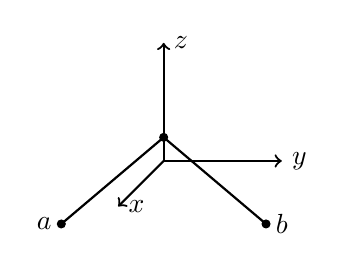
\begin{tikzpicture}
            \draw[thick] (-1.3,-0.8)--(0,0.3)--(1.3,-0.8);
            \draw [->,thick] (0,0)--(0,1.5)node[right]{\(z\)};
            \draw [->,thick] (0,0)--(1.5,0)node[right]{\(y\)};
            \draw [->,thick] (0,0)--(0,0,1.5)node[right]{\(x\)};
            \draw[fill=black] (0,0.3) circle (0.05);
            \draw[fill=black] (-1.3,-0.8) node[left]{\(a\)} circle (0.05);
            \draw[fill=black] (1.3,-0.8) node[right]{\(b\)} circle (0.05);
        \end{tikzpicture}
    \end{figure}

    Let's associate some orbitals and vectors to track what's going on. Consider a nuclear permutation operator \((ab)\) that permutes the labels of the hydrogen nuclei \(a\) and \(b\) only, leaving everything else unchanged. The action of this operator is shown in \cref{nuclear_permutation}. Notice that since the internal frame is defined using the nuclear labels, when we permute the labels, the internal frame also changes its orientation. We can switch our perspective to reorient our system --- then we see that the effect of the \((ab)\) operation on internal coordinates is the same as that of \(C_z^2\), a two-fold rotation along the \(z\) axis that rotates the functions and coordinates only but not the nuclear labels.

    \begin{figure}[ht!]
        \centering
        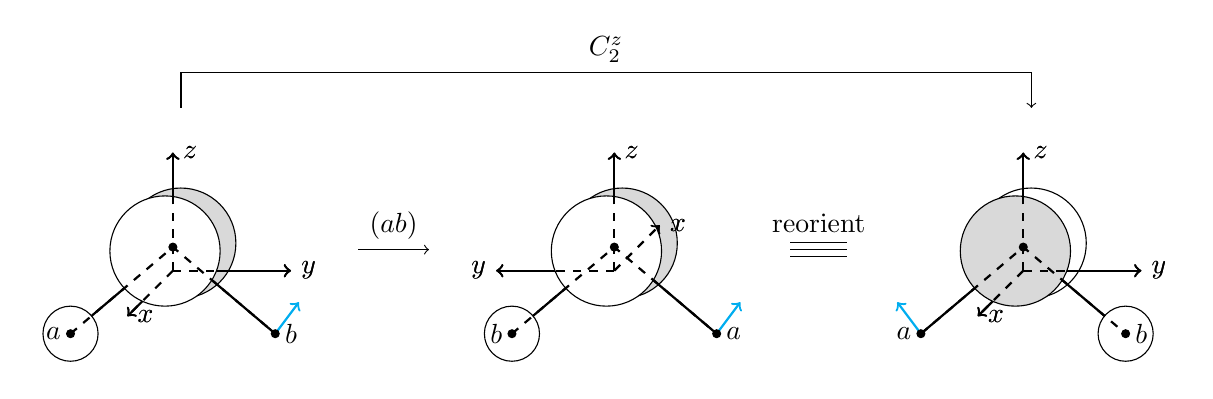
\begin{tikzpicture}[scale=0.9]
            \node at (0,0){\tikz{
                \draw[fill=gray!30] (0.1,0.35) circle (0.7);
                \draw[thick] (-1.3,-0.8)--(0,0.3)--(1.3,-0.8);
                \draw [->,thick] (0,0)--(0,1.5)node[right]{\(z\)};
                \draw [->,thick] (0,0)--(1.5,0)node[right]{\(y\)};
                \draw [->,thick] (0,0)--(0,0,1.5)node[right]{\(x\)};
                \draw[fill=white] (-0.1,0.25) circle (0.7);
                \draw[fill=white] (-1.3,-0.8) circle (0.35);
                \draw [->,thick,dashed] (0,0)--(0,1.5)node[right]{\(z\)};
                \draw [->,thick,dashed] (0,0)--(1.5,0)node[right]{\(y\)};
                \draw [->,thick,dashed] (0,0)--(0,0,1.5)node[right]{\(x\)};
                \draw[thick,dashed] (-1.3,-0.8)--(0,0.3)--(1.3,-0.8);
                \draw[thick,cyan,->] (1.3,-0.8)--(1.6,-0.4);
                \draw[fill=black] (0,0.3) circle (0.05);
                \draw[fill=black] (-1.3,-0.8) node[left]{\(a\)} circle (0.05);
                \draw[fill=black] (1.3,-0.8) node[right]{\(b\)} circle (0.05);
            }};

            \draw[->] (2.5,0)--node[above]{\((ab)\)}(3.5,0);

            \node at (6,0){\tikz{
                \draw[fill=gray!30] (0.1,0.35) circle (0.7);
                \draw[thick] (-1.3,-0.8)--(0,0.3)--(1.3,-0.8);
                \draw [->,thick] (0,0)--(0,1.5)node[right]{\(z\)};
                \draw [->,thick] (0,0)--(-1.5,0)node[left]{\(y\)};
                \draw [->,thick] (0,0)--(0,0,-1.5)node[right]{\(x\)};
                \draw[fill=white] (-0.1,0.25) circle (0.7);
                \draw[fill=white] (-1.3,-0.8) circle (0.35);
                \draw [->,thick,dashed] (0,0)--(0,1.5)node[right]{\(z\)};
                \draw [->,thick,dashed] (0,0)--(-1.5,0)node[left]{\(y\)};
                \draw [->,thick,dashed] (0,0)--(0,0,-1.5)node[right]{\(x\)};
                \draw[thick,dashed] (-1.3,-0.8)--(0,0.3)--(1.3,-0.8);
                \draw[thick,cyan,->] (1.3,-0.8)--(1.6,-0.4);
                \draw[fill=black] (0,0.3) circle (0.05);
                \draw[fill=black] (-1.3,-0.8) node[left]{\(b\)} circle (0.05);
                \draw[fill=black] (1.3,-0.8) node[right]{\(a\)} circle (0.05);
            }};

            \foreach \i in {-1,0,1}{
                \draw (8.6,0.1*\i)--(9.4,0.1*\i);
            }
            \node at (9,0.1)[above]{reorient};

            \node at (12,0){\tikz{
                \draw (0.1,0.35) circle (0.7);
                \draw[thick] (-1.3,-0.8)--(0,0.3)--(1.3,-0.8);
                \draw [->,thick] (0,0)--(0,1.5)node[right]{\(z\)};
                \draw [->,thick] (0,0)--(1.5,0)node[right]{\(y\)};
                \draw [->,thick] (0,0)--(0,0,1.5)node[right]{\(x\)};
                \draw[fill=gray!30] (-0.1,0.25) circle (0.7);
                \draw[fill=white] (1.3,-0.8) circle (0.35);
                \draw [->,thick,dashed] (0,0)--(0,1.5)node[right]{\(z\)};
                \draw [->,thick,dashed] (0,0)--(1.5,0)node[right]{\(y\)};
                \draw [->,thick,dashed] (0,0)--(0,0,1.5)node[right]{\(x\)};
                \draw[thick,dashed] (-1.3,-0.8)--(0,0.3)--(1.3,-0.8);
                \draw[thick,cyan,->] (-1.3,-0.8)--(-1.6,-0.4);
                \draw[fill=black] (0,0.3) circle (0.05);
                \draw[fill=black] (-1.3,-0.8) node[left]{\(a\)} circle (0.05);
                \draw[fill=black] (1.3,-0.8) node[right]{\(b\)} circle (0.05);
            }};

            \draw[->] (0,2)--(0,2.5)--node[above]{\(C_2^z\)}(12,2.5)--(12,2);
        \end{tikzpicture}
        \caption{The action of a nuclear permutation operator \((ab)\) on \(\mathrm{H_2O}\) is equivalent to \(C_2^z\) on associated objects.}
        \label{nuclear_permutation}
    \end{figure}

    Similarly, the action of the parity inversion operator \(E^*\) is the same as acting a \(\sigma_v^{yz}\) to the associated objects (vectors, functions etc.), as shown in \cref{parity_inversion}, and the action of \((ab)E^*\) is the same as \(\sigma_v^{xz}\) to the associated objects as shown in \cref{inversion_permutation}.

    \begin{figure}[ht!]
        \centering
        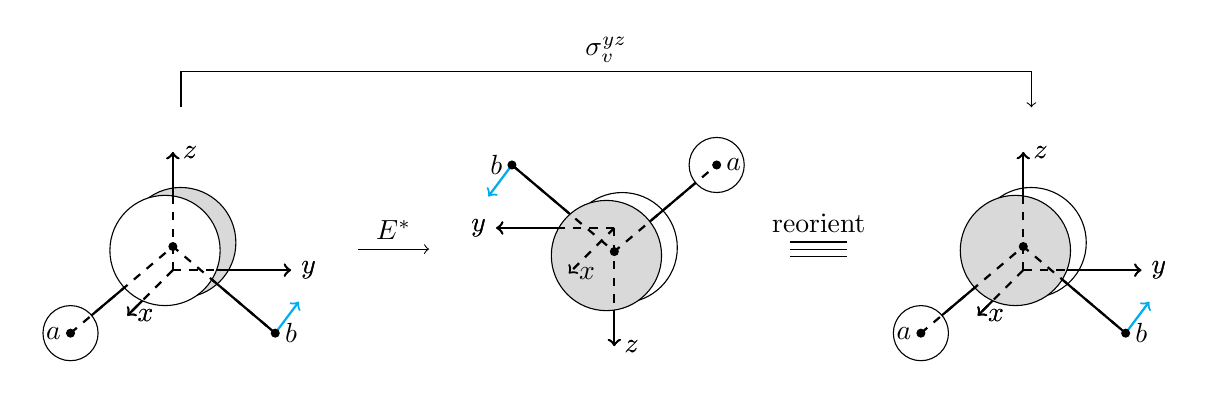
\begin{tikzpicture}[scale=0.9]
            \node at (0,0){\tikz{
                \draw[fill=gray!30] (0.1,0.35) circle (0.7);
                \draw[thick] (-1.3,-0.8)--(0,0.3)--(1.3,-0.8);
                \draw [->,thick] (0,0)--(0,1.5)node[right]{\(z\)};
                \draw [->,thick] (0,0)--(1.5,0)node[right]{\(y\)};
                \draw [->,thick] (0,0)--(0,0,1.5)node[right]{\(x\)};
                \draw[fill=white] (-0.1,0.25) circle (0.7);
                \draw[fill=white] (-1.3,-0.8) circle (0.35);
                \draw [->,thick,dashed] (0,0)--(0,1.5)node[right]{\(z\)};
                \draw [->,thick,dashed] (0,0)--(1.5,0)node[right]{\(y\)};
                \draw [->,thick,dashed] (0,0)--(0,0,1.5)node[right]{\(x\)};
                \draw[thick,dashed] (-1.3,-0.8)--(0,0.3)--(1.3,-0.8);
                \draw[thick,cyan,->] (1.3,-0.8)--(1.6,-0.4);
                \draw[fill=black] (0,0.3) circle (0.05);
                \draw[fill=black] (-1.3,-0.8) node[left]{\(a\)} circle (0.05);
                \draw[fill=black] (1.3,-0.8) node[right]{\(b\)} circle (0.05);
            }};

            \draw[->] (2.5,0)--node[above]{\(E^*\)}(3.5,0);

            \node at (6,0){\tikz{
                \draw[fill=white] (0.1,-0.25) circle (0.7);
                \draw[thick] (-1.3,0.8)--(0,-0.3)--(1.3,0.8);
                \draw [->,thick] (0,0)--(0,-1.5)node[right]{\(z\)};
                \draw [->,thick] (0,0)--(-1.5,0)node[left]{\(y\)};
                \draw [->,thick] (0,0)--(0,0,1.5)node[right]{\(x\)};
                \draw[fill=gray!30] (-0.1,-0.35) circle (0.7);
                \draw[fill=white] (1.3,0.8) circle (0.35);
                \draw [->,thick,dashed] (0,0)--(0,-1.5)node[right]{\(z\)};
                \draw [->,thick,dashed] (0,0)--(-1.5,0)node[left]{\(y\)};
                \draw [->,thick,dashed] (0,0)--(0,0,1.5)node[right]{\(x\)};
                \draw[thick,dashed] (-1.3,0.8)--(0,-0.3)--(1.3,0.8);
                \draw[thick,cyan,->] (-1.3,0.8)--(-1.6,0.4);
                \draw[fill=black] (0,-0.3) circle (0.05);
                \draw[fill=black] (-1.3,0.8) node[left]{\(b\)} circle (0.05);
                \draw[fill=black] (1.3,0.8) node[right]{\(a\)} circle (0.05);
            }};

            \foreach \i in {-1,0,1}{
                \draw (8.6,0.1*\i)--(9.4,0.1*\i);
            }
            \node at (9,0.1)[above]{reorient};

            \node at (12,0){\tikz{
                \draw[fill=white] (0.1,0.35) circle (0.7);
                \draw[thick] (-1.3,-0.8)--(0,0.3)--(1.3,-0.8);
                \draw [->,thick] (0,0)--(0,1.5)node[right]{\(z\)};
                \draw [->,thick] (0,0)--(1.5,0)node[right]{\(y\)};
                \draw [->,thick] (0,0)--(0,0,1.5)node[right]{\(x\)};
                \draw[fill=gray!30] (-0.1,0.25) circle (0.7);
                \draw[fill=white] (-1.3,-0.8) circle (0.35);
                \draw [->,thick,dashed] (0,0)--(0,1.5)node[right]{\(z\)};
                \draw [->,thick,dashed] (0,0)--(1.5,0)node[right]{\(y\)};
                \draw [->,thick,dashed] (0,0)--(0,0,1.5)node[right]{\(x\)};
                \draw[thick,dashed] (-1.3,-0.8)--(0,0.3)--(1.3,-0.8);
                \draw[thick,cyan,->] (1.3,-0.8)--(1.6,-0.4);
                \draw[fill=black] (0,0.3) circle (0.05);
                \draw[fill=black] (-1.3,-0.8) node[left]{\(a\)} circle (0.05);
                \draw[fill=black] (1.3,-0.8) node[right]{\(b\)} circle (0.05);
            }};

            \draw[->] (0,2)--(0,2.5)--node[above]{\(\sigma_v^{yz}\)}(12,2.5)--(12,2);
        \end{tikzpicture}
        \caption{The action of a parity inversion operator \(E^*\) on \(\mathrm{H_2O}\) is equivalent to \(\sigma_v^{yz}\) on associated objects.}
        \label{parity_inversion}
    \end{figure}

    \begin{figure}[ht!]
        \centering
        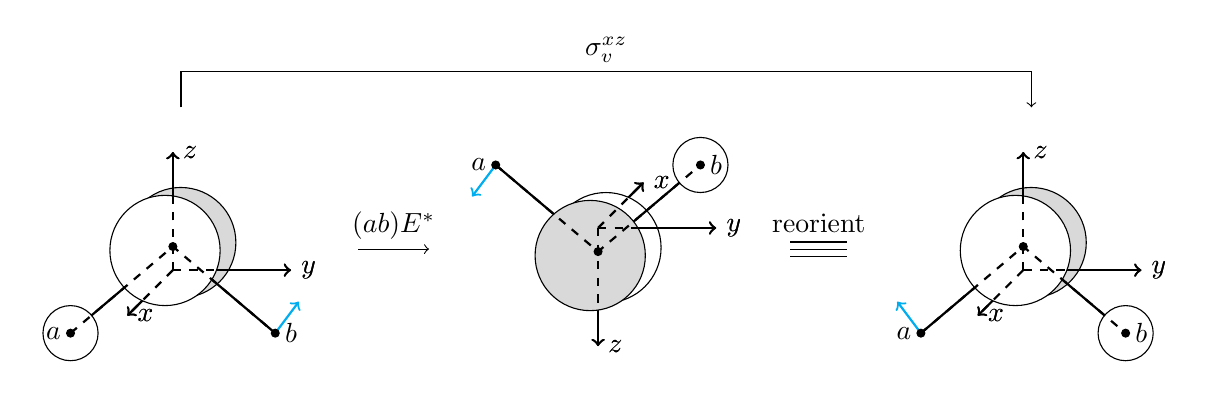
\begin{tikzpicture}[scale=0.9]
            \node at (0,0){\tikz{
                \draw[fill=gray!30] (0.1,0.35) circle (0.7);
                \draw[thick] (-1.3,-0.8)--(0,0.3)--(1.3,-0.8);
                \draw [->,thick] (0,0)--(0,1.5)node[right]{\(z\)};
                \draw [->,thick] (0,0)--(1.5,0)node[right]{\(y\)};
                \draw [->,thick] (0,0)--(0,0,1.5)node[right]{\(x\)};
                \draw[fill=white] (-0.1,0.25) circle (0.7);
                \draw[fill=white] (-1.3,-0.8) circle (0.35);
                \draw [->,thick,dashed] (0,0)--(0,1.5)node[right]{\(z\)};
                \draw [->,thick,dashed] (0,0)--(1.5,0)node[right]{\(y\)};
                \draw [->,thick,dashed] (0,0)--(0,0,1.5)node[right]{\(x\)};
                \draw[thick,dashed] (-1.3,-0.8)--(0,0.3)--(1.3,-0.8);
                \draw[thick,cyan,->] (1.3,-0.8)--(1.6,-0.4);
                \draw[fill=black] (0,0.3) circle (0.05);
                \draw[fill=black] (-1.3,-0.8) node[left]{\(a\)} circle (0.05);
                \draw[fill=black] (1.3,-0.8) node[right]{\(b\)} circle (0.05);
            }};

            \draw[->] (2.5,0)--node[above]{\((ab)E^*\)}(3.5,0);

            \node at (6,0){\tikz{
                \draw [->,thick] (0,0)--(0,0,-1.5)node[right]{\(x\)};
                \draw[fill=white] (0.1,-0.25) circle (0.7);
                \draw[thick] (-1.3,0.8)--(0,-0.3)--(1.3,0.8);
                \draw [->,thick] (0,0)--(0,-1.5)node[right]{\(z\)};
                \draw [->,thick] (0,0)--(1.5,0)node[right]{\(y\)};
                \draw[fill=gray!30] (-0.1,-0.35) circle (0.7);
                \draw[fill=white] (1.3,0.8) circle (0.35);
                \draw [->,thick,dashed] (0,0)--(0,-1.5)node[right]{\(z\)};
                \draw [->,thick,dashed] (0,0)--(1.5,0)node[right]{\(y\)};
                \draw [->,thick,dashed] (0,0)--(0,0,-1.5)node[right]{\(x\)};
                \draw[thick,dashed] (-1.3,0.8)--(0,-0.3)--(1.3,0.8);
                \draw[thick,cyan,->] (-1.3,0.8)--(-1.6,0.4);
                \draw[fill=black] (0,-0.3) circle (0.05);
                \draw[fill=black] (-1.3,0.8) node[left]{\(a\)} circle (0.05);
                \draw[fill=black] (1.3,0.8) node[right]{\(b\)} circle (0.05);
            }};

            \foreach \i in {-1,0,1}{
                \draw (8.6,0.1*\i)--(9.4,0.1*\i);
            }
            \node at (9,0.1)[above]{reorient};

            \node at (12,0){\tikz{
                \draw[fill=gray!30] (0.1,0.35) circle (0.7);
                \draw[thick] (-1.3,-0.8)--(0,0.3)--(1.3,-0.8);
                \draw [->,thick] (0,0)--(0,1.5)node[right]{\(z\)};
                \draw [->,thick] (0,0)--(1.5,0)node[right]{\(y\)};
                \draw [->,thick] (0,0)--(0,0,1.5)node[right]{\(x\)};
                \draw[fill=white] (-0.1,0.25) circle (0.7);
                \draw[fill=white] (1.3,-0.8) circle (0.35);
                \draw [->,thick,dashed] (0,0)--(0,1.5)node[right]{\(z\)};
                \draw [->,thick,dashed] (0,0)--(1.5,0)node[right]{\(y\)};
                \draw [->,thick,dashed] (0,0)--(0,0,1.5)node[right]{\(x\)};
                \draw[thick,dashed] (-1.3,-0.8)--(0,0.3)--(1.3,-0.8);
                \draw[thick,cyan,->] (-1.3,-0.8)--(-1.6,-0.4);
                \draw[fill=black] (0,0.3) circle (0.05);
                \draw[fill=black] (-1.3,-0.8) node[left]{\(a\)} circle (0.05);
                \draw[fill=black] (1.3,-0.8) node[right]{\(b\)} circle (0.05);
            }};

            \draw[->] (0,2)--(0,2.5)--node[above]{\(\sigma_v^{xz}\)}(12,2.5)--(12,2);
        \end{tikzpicture}
        \caption{The action of a parity inversion operator \((ab)E^*\) on \(\mathrm{H_2O}\) is equivalent to \(\sigma_v^{xz}\) on associated objects.}
        \label{inversion_permutation}
    \end{figure}

    \subsubsection{Allowed Rotational States of Molecules}
    We can expand the total wavefunction of a molecule into a product of electronic, vibrational, rotational, translational and nuclear spin factors
    \begin{equation}
        \Psi=\psi_{\text{elec}}\psi_{\text{vib}}\psi_{\text{rot}}\psi_{\text{trans}}\psi_{\text{ns}}\,.
    \end{equation}
    However, recall that Pauli principle requires the wavefunction to be symmetric with respect to the exchange of identical Bosons (integer-spin nuclei) and antisymmetric with respect to the exchange of identical Fermions (electrons and half-integer-spin nuclei). This means that we cannot combine any components of the wavefunction with each other --- we must maintain the overall symmetry/antisymmetry.

    \subsubsection*{Ortho and Para Hydrogen}
    Let's consider a ground electronic and vibrational state \(\mathrm{H}_2\) molecule with the two nuclei labelled by \(a\) and \(b\). What happens if we perform the symmetry operator \((ab)\) which exchanges the proton labels?

    The ground state electronic state of \(\mathrm{H}_2\) is \(^1\Sigma_g^+\), i.e. totally symmetric, so it is unchanged by \((ab)\). The vibrational wavefunction only depends on the bond length \(\norm{\vb{r}_a-\vb{r}_b}\), which is unchanged by the exchange of the labels \(a\) and \(b\). The translational wavefunction only depends on the overall (centre of mass) position of the molecule. It is also unchanged by \((ab)\).
    
    However, \(\psi_{\text{rot}}\) is a spherical harmonic \(Y_{JM}(\theta,\varphi)\), where \(\theta\) and \(\varphi\) describes the orientation of the molecule in the global frame. This orientation of the molecule is reversed when \(a\) and \(b\) are interchanged. For example, if we define the direction of the molecule to be from \(a\) to \(b\), and its currently pointing in direction \((\theta,\phi)\) in the global frame, then permuting the labels \(a\) and \(b\) would make the molecule point in the reverse direction \(\pi-\theta,\pi+\varphi\). As a result, the rotational wavefunction changes sign if \(J\) is odd, and is unchanged if \(J\) is even under such an inversion.\footnote{The easiest way to confirm this without using mathematics is to check the angular parts of the atomic orbitals. \(J=0\) is the \(s\) orbitals, \(J=1\) is the \(p\) orbitals and \(J=2\) is the \(d\) orbitals etc. If you are not convinced by this, you can check that the spherical harmonics have the general expression
    \begin{equation}
        Y_{\ell m}=\sqrt{\frac{2\ell+1}{4\pi}\frac{(\ell-m)!}{(\ell+m)!}}P_\ell^{\abs{m}}(\cos\theta)\ee^{\ii m\varphi}\,,
    \end{equation}
    where \(P_\ell^m\) is the associated Legendre polynomial, defined by
    \begin{align}
        P_\ell^{\abs{m}}(x)&=(-1)^{\abs{m}}(1-x^2)^{\abs{m}/2}\dv[\abs{m}]{}{x}(P_\ell (x))\,,\\
        P_\ell(x)&=\frac{1}{2^\ell \ell!}\dv[\ell]{}{x}(x^2-1)^\ell\,.
    \end{align}
    The inversion is described by the change of coordinate \((\theta,\varphi)\mapsto(\pi-\theta,\pi+\varphi)\). One can straightforwardly confirm that \(P_\ell(-x)=(-1)^\ell P_\ell(x)\), and so \(P_\ell^{\abs{m}}(-x)=(-1)^{\ell-\abs{m}}P_\ell^{\abs{m}}(x)\). Therefore we get the claimed result \(Y_{\ell,m}(\pi-\theta,\pi+\varphi)=(-1)^{\ell}Y_{\ell,m}(\theta,\varphi)\).}

    Finally, the spin of hydrogen is \(I=1/2\), so the nuclear spin function of \(\mathrm{H_2}\) is either a singlet
    \begin{equation}
        \psi_{\text{singlet}}=\sqrt{\frac{1}{2}}(\alpha_a\beta_b-\beta_a\alpha_b)
    \end{equation}
    that is antisymmetric with respect to \((ab)\), or one of the triplet functions
    \begin{equation}
        \psi_{\text{triplet}}=\begin{cases}
            \alpha_a\alpha_b \\
            \sqrt{\frac{1}{2}}(\alpha_a\beta_b+\beta_a\alpha_b) \\
            \beta_a\beta_b
        \end{cases}
    \end{equation}
    that are symmetric with respect to \((ab)\). Because the nuclear spins interact only very weakly with the environment, the spin states do not change easily. We can speak of \textit{ortho hydrogen} for the ones with triplet nuclear spin, and \textit{para hydrogen} for those with singlet nuclear spin.

    Therefore, to maintain the overall antisymmetry of the total wavefunction when we perform the permutation of the two Fermion nuclei \(a\) and \(b\), the ortho hydrogen with symmetric spins must combine with odd \(J\) rotational states, while the para hydrogen with antisymmetric spins must have even rotational states. This can be confirmed in Raman spectrum. Since there are three times as many ortho hydrogen as para at equilibrium at high temperatures due to nuclear spin degeneracy, the rotational Raman spectra of \(\mathrm{H_2}\) show alternating intensities of \(3:1\) between odd and even \(J\).

    \subsubsection*{Carbon Dioxide}
    In \(\mathrm{CO_2}\), \(\mathrm{O}\) has \(I=0\), so the nuclear spin function is trivially \(\psi_{\text{ns}}=1\). The wavefunction is symmetric with respect to the exchange of the labels of the two Bosonic oxygens, so only even \(J\) rotational functions are allowed --- odd-\(J\) peaks are absent in the rotational and vibration-rotational Raman spectra of \(\mathrm{CO_2}\).

    \subsubsection*{Oxygen}
    The oxygen molecule has a more interesting ground electronic state of \(^3\Sigma_g^-\). The minus sign means that the electronic wavefunction changes its sign upon reflection about a mirror plane that contains the principal axis. When we exchange \(a\) and \(b\), we inverted the direction of the \(z\) axis, and to maintain the right-handedness of the internal coordinate system, we must also do such a mirror plane reflection to permute the \(x\) and \(y\) axis. Hence, the electronic wavefunction changes its sign under \((ab)\). The nuclear wavefunction is symmetric under \((ab)\). As a result, to obey Pauli principle, the rotational wavefunction of \(\mathrm{O_2}\) must have odd \(J\).

    \newpage
    \section{Groups}
    \begin{defn}
        A \textit{group} is a triple \((G,\ \cdot\ ,E)\) of a set \(G\), a binary operation \(\ \cdot \ : G\times G\to G\) often known as the \textit{group product}, and an element \(E\in G\) such that the following axioms are satisfied:\footnote{Some authors may include \textit{closure} as one of the group axioms --- this is stupid. Closure is naturally guaranteed by the definition of a binary operation.}
        \begin{enumerate}[topsep=0pt]
            \item \textit{Associativity}: \((R\cdot S)\cdot T=R\cdot(S\cdot T)\) \(\forall R,S,T\in G\). This allows us to write both as \(R\cdot S\cdot T\) directly without ambiguity.
            \item \textit{Identity}: The \textit{identity element} \(E\) satisfies \(R\cdot E=E\cdot R=R\) for all \(R\in G\).
            \item \textit{Inverse}: For every \(R\in G\), there is an \textit{inverse} \(R^{-1}\in G\) such that \(R\cdot R^{-1}=R^{-1}\cdot R=E\).
        \end{enumerate}
    \end{defn}

    Groups naturally arise when studying symmetries, because the symmetry operations of a certain system naturally form a group. If you perform a symmetry operation, then perform another, then the combined action is another symmetry operation. This defines the group product. Doing nothing is a symmetry operation --- this is the identity. Whatever symmetry operation you perform, you can always undo it. This reverse operation is the inverse.

    To better investigate the symmetry of objects using group theory, we need to let the group elements (the symmetry operations) to act on some object (the object that we wish to describe the symmetry of). This leads to the definition of a group action.
    \begin{defn}
        Let \((G, \ \cdot \ , E)\) be a group and \(X\) be a set. A \textit{group action} \(*\) of \(G\) on \(X\) is a map \(*:G\times X\to X\) that satisfies the following axioms
        \begin{enumerate}[topsep=0pt]
            \item \textit{Identity}. \(E*x=x\) \(\forall x\in X\).
            \item \textit{Compatibility}. \(R*(S*x)=(R\cdot S)*x\) \(\forall R,S\in G, x\in X\).
        \end{enumerate}
    \end{defn}

    \begin{ex}
        Consider the rotational symmetry of a triangle. The group of the symmetry operations is \(G=\{E, C_3, C_3^2\}\), and the set that group \(G\) is acting on is
        \begin{equation}
            X=\left\{\tikz[baseline=0.8em]{
                \draw(0,0)--(1,0)--(0.5,0.866)--(0,0);
                \draw[fill=white] (0,0) circle (0.05);
                \draw[fill=white] (1,0) circle (0.05);
                \draw[fill=black] (0.5,0.866) circle (0.05);
            }\,,\,\tikz[baseline=0.8em]{
                \draw(0,0)--(1,0)--(0.5,0.866)--(0,0);
                \draw[fill=black] (0,0) circle (0.05);
                \draw[fill=white] (1,0) circle (0.05);
                \draw[fill=white] (0.5,0.866) circle (0.05);
            }\,,\,\tikz[baseline=0.8em]{
                \draw(0,0)--(1,0)--(0.5,0.866)--(0,0);
                \draw[fill=white] (0,0) circle (0.05);
                \draw[fill=black] (1,0) circle (0.05);
                \draw[fill=white] (0.5,0.866) circle (0.05);
            }\right\}\,.
        \end{equation}
        Then we have, for example,
        \begin{equation}
            E*\tikz[baseline=0.8em]{
                \draw(0,0)--(1,0)--(0.5,0.866)--(0,0);
                \draw[fill=white] (0,0) circle (0.05);
                \draw[fill=white] (1,0) circle (0.05);
                \draw[fill=black] (0.5,0.866) circle (0.05);
            }=\tikz[baseline=0.8em]{
                \draw(0,0)--(1,0)--(0.5,0.866)--(0,0);
                \draw[fill=white] (0,0) circle (0.05);
                \draw[fill=white] (1,0) circle (0.05);
                \draw[fill=black] (0.5,0.866) circle (0.05);
            }\,.
        \end{equation}
        \begin{equation}
            C_3*\tikz[baseline=0.8em]{
                \draw(0,0)--(1,0)--(0.5,0.866)--(0,0);
                \draw[fill=white] (0,0) circle (0.05);
                \draw[fill=white] (1,0) circle (0.05);
                \draw[fill=black] (0.5,0.866) circle (0.05);
            }=\tikz[baseline=0.8em]{
                \draw(0,0)--(1,0)--(0.5,0.866)--(0,0);
                \draw[fill=black] (0,0) circle (0.05);
                \draw[fill=white] (1,0) circle (0.05);
                \draw[fill=white] (0.5,0.866) circle (0.05);
            }\,.
        \end{equation}
        \begin{align}
            C_3*\left(C_3*\tikz[baseline=0.8em]{
                \draw(0,0)--(1,0)--(0.5,0.866)--(0,0);
                \draw[fill=white] (0,0) circle (0.05);
                \draw[fill=white] (1,0) circle (0.05);
                \draw[fill=black] (0.5,0.866) circle (0.05);
            }\right)&=C_3*\tikz[baseline=0.8em]{
                \draw(0,0)--(1,0)--(0.5,0.866)--(0,0);
                \draw[fill=black] (0,0) circle (0.05);
                \draw[fill=white] (1,0) circle (0.05);
                \draw[fill=white] (0.5,0.866) circle (0.05);
            }=\tikz[baseline=0.8em]{
                \draw(0,0)--(1,0)--(0.5,0.866)--(0,0);
                \draw[fill=white] (0,0) circle (0.05);
                \draw[fill=black] (1,0) circle (0.05);
                \draw[fill=white] (0.5,0.866) circle (0.05);
            }\\
            &=C_3^2*\tikz[baseline=0.8em]{
                \draw(0,0)--(1,0)--(0.5,0.866)--(0,0);
                \draw[fill=white] (0,0) circle (0.05);
                \draw[fill=white] (1,0) circle (0.05);
                \draw[fill=black] (0.5,0.866) circle (0.05);
            }=\tikz[baseline=0.8em]{
                \draw(0,0)--(1,0)--(0.5,0.866)--(0,0);
                \draw[fill=white] (0,0) circle (0.05);
                \draw[fill=black] (1,0) circle (0.05);
                \draw[fill=white] (0.5,0.866) circle (0.05);
            }
        \end{align}
        In the last equation, the first line computed the two actions separately, while in the second line we take the group product first. This shows the compatibility axiom. 
    \end{ex}

    From now on, we use the notation \(*\) for group action exclusively to avoid confusion. We will also sometimes omit \(\ \cdot\ \) or \(*\) when what we are doing is clear from the context. However, note that \(RS\psi\) means \(R*(S*\psi)\). We act \(S\) on \(\psi\) first, and then act \(R\) on the result of \(S*\psi\).

    \begin{defn}
        A group \(G\) is \textit{finite} if \(G\) consists of a finite number of elements. The \textit{order} of a finite group is the number of elements in it.
    \end{defn}
    \begin{defn}
        A group \(G\) is \textit{Abelian} if \(\forall R,S\in G\), \(RS=SR\), i.e. the group product is commutative.
    \end{defn}

    If a group is finite, then we can clearly list all possible results of the product of any two elements. If we construct a table by putting the first argument of the group product in rows, and the second argument of a group product in columns, then we obtain a \textit{multiplication table.}

    \begin{ex}
        \textit{The multiplication table of \(D_3\).}

        We define the symmetry operations on a dihedral triangle as shown in the diagram below.
        \begin{figure}[ht!]
            \centering
            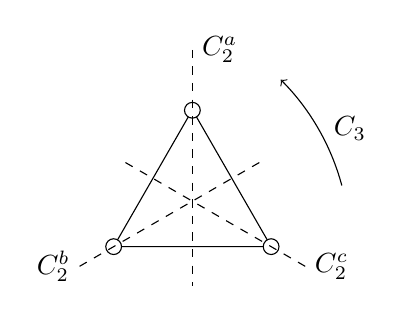
\begin{tikzpicture}
                \draw (0,0)--(2,0)--(1,1.738)--(0,0);
                \draw[fill=white] (0,0) circle (0.1);
                \draw[fill=white] (2,0) circle (0.1);
                \draw[fill=white] (1,1.732) circle (0.1);
                \draw[dashed] (1,2.5)node[right]{\(C_2^a\)}--(1,-0.5);
                \draw[dashed] (-0.433,-0.25)node[left]{\(C_2^b\)}--(1.933,1.116);
                \draw[dashed] (2.433,-0.25)node[right]{\(C_2^c\)}--(0.067,1.116);
                \draw[->] (2.898,0.776) arc (15:45:3);
                \node at (3,1.5) {\(C_3\)};
            \end{tikzpicture}
        \end{figure}

        Then the symmetries form a \(D_3\) group, whose group table can be obtained as follows.
        \begin{table}[ht!]
            \centering\renewcommand{\arraystretch}{1.3}
            \begin{tabular}{c|cccccc}
                ~ & \(E\) & \(C_3\) & \(C_3^2\) & \(C_2^a\) & \(C_2^b\) & \(C_2^c\) \\ \hline
                \(E\) & \(E\) & \(C_3\) & \(C_3^2\) & \(C_2^a\) & \(C_2^b\) & \(C_2^c\) \\
                \(C_3\) & \(C_3\) & \(C_3^2\) & \(E\) & \color{blue}\(C_2^c\) & \(C_2^a\) & \(C_2^b\) \\
                \(C_3^2\) & \(C_3^2\) & \(E\) & \(C_3\) & \(C_2^b\) & \(C_2^c\) & \(C_2^a\) \\
                \(C_2^a\) & \(C_2^a\) & \color{red}\(C_2^b\) & \(C_2^c\) & \(E\) & \(C_3\) & \(C_3^2\) \\
                \(C_2^b\) & \(C_2^b\) & \(C_2^c\) & \(C_2^a\) & \(C_3^2\) & \(E\) & \(C_3\) \\
                \(C_2^c\) & \(C_2^c\) & \(C_2^a\) & \(C_2^b\) & \(C_3\) & \(C_3^2\) & \(E\)
            \end{tabular}
        \end{table}
        
        For example, the entry marked in blue means that
        \begin{equation}
            C_3 C_2^a=C_2^c\,,
        \end{equation}
        i.e. if you flip the triangle along the axis \(a\), then rotate \(120^\circ\) along the principal axis anticlockwise, then the overall effect is equivalent to flipping the triangle along the axis \(c\). However, if you do the two operations in a reverse order, then what you get is the entry marked in red
        \begin{equation}
            C_2^a C_3=C_2^b\,.
        \end{equation}
        This clearly shows that the \(D_3\) group is not Abelian --- the order of operations matters.
    \end{ex}

    \begin{defn}
        A group is said to be \textit{generated} by a subset of its elements if all the group elements can be produced by performing group products within this subset of elements.
    \end{defn}
    \begin{ex}
        \textit{The cyclic group \(C_n\).}

        Consider the rotational symmetry of a regular \(n\)-gon. The cyclic group of order \(n\), denoted \(C_n\), contains all the rotational symmetry operations, i.e. rotations by \(360^\circ k/n\) for \(k=1,\dots, n\). We denote the rotation of \(360^\circ/n\) as \(R\), then we see that the group \(C_n\) is generated by \(R\), since all the group elements can be written as \(R^k\), and in particular, the identity element \(E=R^n\).
    \end{ex}

    A lot of groups are generated by more than one elements. For example, you can check that \(D_3\) is generated by \(\{C_3,C_2^a\}\).

    \begin{defn}
        If \((G,\ \cdot\ , E)\) is a group, then \((H,\ \cdot\ , E)\) is a \textit{subgroup} of \(G\), denoted \(H\le G\), if \(H\) is a non-empty subset of \(G\), and \(H\) is a group on its own under the same group product \(\ \cdot\ \).
    \end{defn}

    \begin{ex}
        \(C_3\le D_3\). This is evident from the group multiplication table.
        \begin{table}[ht!]
            \centering\renewcommand{\arraystretch}{1.3}
            \begin{tabular}{c|cccccc}
                ~ & \(E\) & \(C_3\) & \(C_3^2\) & \(C_2^a\) & \(C_2^b\) & \(C_2^c\) \\ \hline
                \(E\) & \(E\) & \(C_3\) & \(C_3^2\) & \(C_2^a\) & \(C_2^b\) & \(C_2^c\) \\
                \(C_3\) & \(C_3\) & \(C_3^2\) & \(E\) & \(C_2^c\) & \(C_2^a\) & \(C_2^b\) \\
                \(C_3^2\) & \(C_3^2\) & \(E\) & \(C_3\) & \(C_2^b\) & \(C_2^c\) & \(C_2^a\) \\
                \(C_2^a\) & \(C_2^a\) & \(C_2^b\) & \(C_2^c\) & \(E\) & \(C_3\) & \(C_3^2\) \\
                \(C_2^b\) & \(C_2^b\) & \(C_2^c\) & \(C_2^a\) & \(C_3^2\) & \(E\) & \(C_3\) \\
                \(C_2^c\) & \(C_2^c\) & \(C_2^a\) & \(C_2^b\) & \(C_3\) & \(C_3^2\) & \(E\)
            \end{tabular}
            \begin{tikzpicture}[overlay]
                \draw[red,thick] (-6.2,-0.2) rectangle (-2.8,2);
            \end{tikzpicture}
        \end{table}
    \end{ex}

    \begin{defn}
        Let \((G,\ \cdot_G\ ,E)\) and \((H,\ \cdot_H \ ,I)\) be groups. Then the \textit{direct product group} \(P=G\times H\) is a group whose elements are \(P=\{(g,h)\mid g\in G,h\in H\}\), and the group product \(\circ\) is defined by
        \begin{equation}
            (g_1,h_1)\circ(g_2,h_2)=(g_1\cdot_G g_2,h_1\cdot_H h_2)\,.
        \end{equation}
    \end{defn}
    We can prove some properties of the direct product group.
    \begin{prop}
        Let \((G,\ \cdot_G\ ,E)\) be a group of order \(n_G\) and \((H,\ \cdot_H\ ,I)\) be a group of order \(n_H\). Let \(P=G\times H\). Consider the following subsets of \(P\):
        \begin{equation}
            G'=\{(g,I)\mid g\in G\}\quad\text{and}\quad H'=\{(E,h)\mid h\in H\}\,.
        \end{equation}
        We have
        \begin{enumerate}[topsep=0pt,label=(\roman*)]
            \item The order of \(P\) is \(n_G n_H\).
            \item \(G'\), \(H'\) are subgroups of \(P\).
            \item \(G'\) is the same group as \(G\), and \(H'\) is the same group as \(H\).
            \item \(G'\cap H'=\{(E,I)\}\).
            \item Every element of \(P\) can be expressed as the product of an element in \(G'\) and an element in \(H'\).
            \item Every element in \(G'\) commutes with every element in \(H'\).
        \end{enumerate}
    \end{prop}
    \begin{proofskip}
        \begin{enumerate}[topsep=0pt,label=(\roman*)]
            \item There are \(n_G\) elements in \(G\) and \(n_H\) elements in \(H\), so we can construct \(n_G n_H\) distinct pairs.
            \item \(G',H'\) are clearly subsets of \(P\). \(G'\) is closed because \((g_1,I)\circ (g_2,I)=(g_1\cdot_G g_2,I)\), which is by definition in \(P\) because \(g_1\cdot_G g_2\in G\). The inverse of \((g_1,I)\in G\) is \((g_1^{-1},I)\in G\). \(G'\) is indeed a group, so it is a subgroup. The same for \(H'\).
            \item There is a one-to-one correspondence between elements in \(G\) and the elements in \(G'\). If we identify \((g,I)\in G'\) as \(g\in G\), then clearly \(G'\) and \(G\) are the same. Mathematically, we say \(G\) and \(G'\) are \textit{isomorphic}, meaning that they are essentially the same group. Same for \(H'\).
            \item Obvious.
            \item \((g,h)=(g,I)\circ(E,h)\).
            \item \((g,I)\circ(E,h)=(g,h)=(E,h)\circ(g,I)\).\qed
        \end{enumerate}
    \end{proofskip}
    We can see that the direct product is the simplest possible way to build up large groups from smaller groups. But more importantly, sometimes we may find that some larger groups are in fact the direct product of some smaller groups. In that case, we may treat the symmetry of its component groups individually.

    Moreover, we can see that the conditions (iv), (v) and (vi) above uniquely determine the algebraic structure of the direct product \(P\). That is, if \(P\) is any group, and we have found two subgroups \(G\) and \(H\) that satisfy the properties above, then \(P\) is necessarily the direct product of \(G\) and \(H\). In this situation, \(P\) is sometimes referred to as the \textit{internal direct product} of its subgroups \(G\) and \(H\).

    \begin{ex}
        \(D_{3h}=D_3\times C_s\), via
        \begin{table}[ht!]
            \centering\renewcommand{\arraystretch}{1.3}
            \begin{tabular}{c|cccccc}
                ~ &\(E\) & \(C_3\) & \(C_3^2\) & \(C_2^a\) & \(C_2^b\) & \(C_2^c\) \\ \hline
                \(E\) & \(E\) & \(C_3\) & \(C_3^2\) & \(C_2^a\) & \(C_2^b\) & \(C_2^c\) \\
                \(\sigma_h\) & \(\sigma_h\) & \(S_3\) & \(S_3^2\) & \(\sigma_v^a\) & \(\sigma_v^b\) & \(\sigma_v^c\)
            \end{tabular}
        \end{table}
    \end{ex}
    
    \begin{defn}
        Two elements \(R,S\in G\) are \textit{equivalent}, denoted \(R\sim S\), if there exists \(Q\in G\) such that
        \begin{equation}
            S=QRQ^{-1}\,.
        \end{equation}
    \end{defn}

    The operator \(QRQ^{-1}\) can be thought of the operator obtained by applying \(Q\) to the operator \(R\) itself. For example, in \(D_{3}\) group,
    \begin{equation}
        C_3C_2^a C_3^{-1}= C_2^b\,,
    \end{equation}
    so \(C_2^a\sim C_2^b\). The rotational axis of \(C_2^b\) that of \(C_2^a\), rotated by \(C_3\).

    However, not all operations ``of the same type'' are equivalent. For example, in \(C_{2v}\), there is no symmetry operation that transforms the \(\sigma_v^{xz}\) plane to the \(\sigma_v^{yz}\) plane.

    \begin{prop}
        Let \(G\) be a group.
        \begin{enumerate}[topsep=0pt,label=(\roman*)]
            \item \textit{Reflexivity}. \(S\sim S\).
            \item \textit{Symmetry}. If \(S\sim R\), then \(R\sim S\).
            \item \textit{Transitivity}. If \(S\sim R\) and \(R\sim T\), then \(S\sim T\).
        \end{enumerate}
    \end{prop}
    \begin{proofskip}
        \begin{enumerate}[topsep=0pt,label=(\roman*)]
            \item \(S=ESE^{-1}\).
            \item If \(S=QRQ^{-1}\), then \(R=Q^{-1}SQ\).
            \item If \(R=PSP^{-1}\) and \(S=QTQ^{-1}\), then \(R=(PQ)T(PQ)^{-1}\).\qed
        \end{enumerate}
    \end{proofskip}
    This allows us to partition the group elements into \textit{conjugacy classes}, so that all elements in the same class are equivalent to each other, but elements from two different classes are inequivalent.

    Note that in any group, the identity always forms a conjugacy class by itself, because for any \(Q\), \(QEQ^{-1}=E\). Note also that in an Abelian group, every element forms a class by itself, since for any \(Q,R\), \(QRQ^{-1}=QQ^{-1}R=R\).

    \newpage
    \section{Representations}
    \subsection{Matrix Representations}
    When we think of a group, we think of it as a collection of symmetry operations that we can act on a physical object. But naturally, the operations we can do to an object, such as rotations and inversions, can also be described by linear transformations if we consider the object to be embedded in a vector space.

    Let's consider the rotational symmetries of a triangle, which forms the \(C_3\) group. To consider the action of the \(C_3\) group operations on the triangle, we put it into a two dimensional vector space, with the centre of mass at the origin and one of the unit vectors (say \(\vu{\imath}\)) parallel to one of the sides.

    \begin{figure}[ht!]
        \centering
        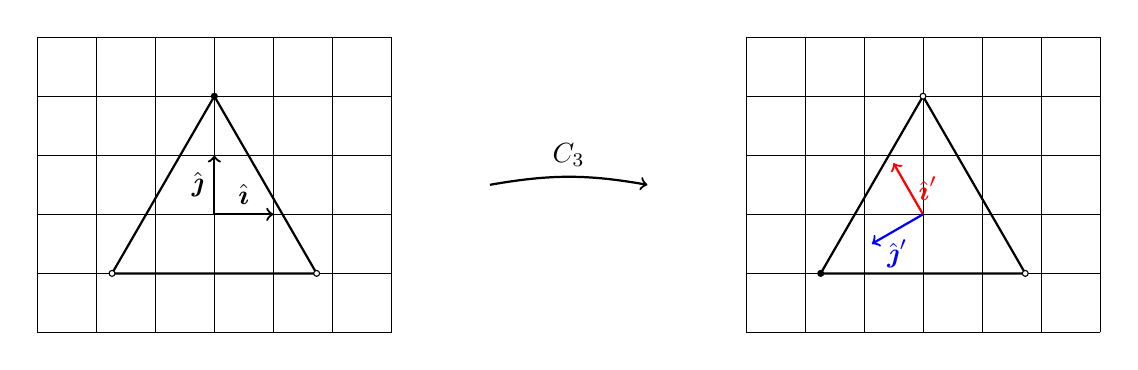
\begin{tikzpicture}
            \node at (0,0){\tikz[scale=0.75]{
                \draw[step=1cm,very thin] (-3,-2) grid (3,3);
                \draw[thick] (0,2)--(1.732,-1)--(-1.732,-1)--(0,2);
                \draw[fill=black] (0,2) circle (0.05);
                \draw[fill=white] (1.732,-1) circle (0.05);
                \draw[fill=white] (-1.732,-1) circle (0.05);
                \draw[->,thick] (0,0)--node[above]{\(\vu{\imath}\)}(1,0);
                \draw[->,thick] (0,0)--node[left]{\(\vu{\jmath}\)}(0,1);
            }};
            \draw[thick,->] (3.5,0)to[bend left=10]node[above]{\(C_3\)} (5.5,0);
            \node at (9,0){\tikz[scale=0.75]{
                \draw[step=1cm,very thin] (-3,-2) grid (3,3);
                \draw[thick] (0,2)--(1.732,-1)--(-1.732,-1)--(0,2);
                \draw[fill=white] (0,2) circle (0.05);
                \draw[fill=white] (1.732,-1) circle (0.05);
                \draw[fill=black] (-1.732,-1) circle (0.05);
                \draw[->,red,thick] (0,0)--+(120:1)node[midway,right]{\(\vu{\imath}'\)};
                \draw[->,blue,thick] (0,0)--+(210:1)node[midway,below]{\(\vu{\jmath}'\)};
            }};
        \end{tikzpicture}
    \end{figure}

    Then to act a \(C_3\) operation to the triangle, we can rotate the underlying vector space by \(120^\circ\). This operation sends the unit vector \(\vu{\imath}\) to \(\vu{\imath}'=-\frac{1}{2}\vu{\imath}+\frac{\sqrt{3}}{2}\vu{\jmath}\), and sends \(\vu{\jmath}\) to \(\vu{\jmath}'=-\frac{\sqrt{3}}{2}\vu{\imath}-\frac{1}{2}\vu{\jmath}\). Mathematically, this means that we can describe this by a transformation matrix
    \begin{equation}
        \DD(C_3)=\begin{pmatrix}
            -\frac{1}{2} & -\frac{\sqrt{3}}{2} \\
            \frac{\sqrt{3}}{2} & -\frac{1}{2}
        \end{pmatrix}
    \end{equation}
    since this operation transform the basis by
    \begin{equation}
        C_3*\begin{pmatrix}
            \vu{\imath} & \vu{\jmath}
        \end{pmatrix}=\begin{pmatrix}
            \vu{\imath}' & \vu{\jmath}'
        \end{pmatrix}=\begin{pmatrix}
            \vu{\imath} & \vu{\jmath}
        \end{pmatrix}\begin{pmatrix}
            -\frac{1}{2} & -\frac{\sqrt{3}}{2} \\
            \frac{\sqrt{3}}{2} & -\frac{1}{2}
        \end{pmatrix}\,.
    \end{equation}
    Then for any vector
    \begin{equation}
        \vb{v}=v_x\vu{\imath}+v_y\vu{\jmath}=\begin{pmatrix}
            \vu{\imath} & \vu{\jmath}
        \end{pmatrix}\begin{pmatrix}
            v_x \\ v_y
        \end{pmatrix}\,,
    \end{equation}
    we have
    \begin{align}
        C_3*\vb{v}&=C_3*\begin{pmatrix}
            \vu{\imath} & \vu{\jmath}
        \end{pmatrix}\begin{pmatrix}
            v_x \\ v_y
        \end{pmatrix}\notag \\
        &=\begin{pmatrix}
            \vu{\imath} & \vu{\jmath}
        \end{pmatrix}\begin{pmatrix}
            -\frac{1}{2} & -\frac{\sqrt{3}}{2} \\
            \frac{\sqrt{3}}{2} & -\frac{1}{2}
        \end{pmatrix}\begin{pmatrix}
            v_x \\ v_y
        \end{pmatrix}\,.
    \end{align}

    Similarly, to act the operation \(C_3^2\) to the triangle, one can rotate the underlying vector space by \(240^\circ\). This corresponds to a basis transformation matrix
    \begin{equation}
        \DD(C_3^2)=\begin{pmatrix}
            -\frac{1}{2} & \frac{\sqrt{3}}{2} \\
            -\frac{\sqrt{3}}{2} & -\frac{1}{2}
        \end{pmatrix}\,,
    \end{equation}
    since the transformed basis is
    \begin{equation}
        \begin{pmatrix}
            \vu{\imath}'' & \vu{\jmath}''
        \end{pmatrix}=\begin{pmatrix}
            \vu{\imath} & \vu{\jmath}
        \end{pmatrix}\begin{pmatrix}
            -\frac{1}{2} & \frac{\sqrt{3}}{2} \\
            -\frac{\sqrt{3}}{2} & -\frac{1}{2}
        \end{pmatrix}\,.
    \end{equation}
    Moreover, the identity operation does nothing to the vector space, and so it corresponds to the identity matrix
    \begin{equation}
        \DD(E)=\begin{pmatrix}
            1 & 0 \\
            0 & 1
        \end{pmatrix}\,.
    \end{equation}

    We have obtained a set of matrices, each corresponds to an operation in the group \(C_3\). A natural consequence is that doing two group operations to the triangle is equivalent to doing two corresponding actions on the underlying vector space. For example, since \(C_3\cdot C_3^2=E\), transforming the underlying vector space by rotation of \(240^\circ\), then \(120^\circ\) is equivalent to doing nothing, so we naturally have the corresponding relationship for the transformation matrices
    \begin{equation}
        \DD(C_3)\DD(C_3^2)=\DD(E)\,.
    \end{equation}

    What we have done above is to use a set of matrices to \textit{represent} the elements in the \(C_3\) group, such that the for any relationship of group elements under group product \(R\cdot S=T\), we have the corresponding relationship for the representation matrices under matrix multiplication
    \begin{equation}
        \DD(R)\DD(S)=\DD(T)\,.
    \end{equation}
    This is because for any vector \(\vb{v}=v_x\vu{\imath}+v_y\vu{\jmath}\), we have
    \begin{align}
        R*(S*\vb{v})&=R*\begin{pmatrix}
            \vu{\imath} & \vu{\jmath}
        \end{pmatrix}\DD(S)\begin{pmatrix}
            v_x \\ v_y
        \end{pmatrix}\notag\\
        &=\begin{pmatrix}
            \vu{\imath} & \vu{\jmath}
        \end{pmatrix}\DD(R)\DD(S)\begin{pmatrix}
            v_x \\ v_y
        \end{pmatrix}\,,
    \end{align}
    while by the compatibility of group actions, we also have
    \begin{equation}
        R*(S*\vb{v})=(R\cdot S)*\vb{v}=\begin{pmatrix}
            \vu{\imath} & \vu{\jmath}
        \end{pmatrix}\DD(R\cdot S)\begin{pmatrix}
            v_x \\ v_y
        \end{pmatrix}\,.
    \end{equation}

    Mathematically, what we are constructing here is called a \textit{homomorphism}.
    \begin{defn}
        Let \((G,\ \cdot\ ,E)\) and \((H,\circ,I)\) be groups. A function \(\phi:G\to H\) is a \textit{homomorphism} if for all \(R,S\in G\),
        \begin{equation}
            \phi(R)\circ\phi(S)=\phi(R\cdot S)\,.
        \end{equation}
    \end{defn}
    You can check that the set of all \(n\times n\) invertible matrices with real entries form a group under matrix multiplication, which is often called the \textit{general linear group}, denoted \(\GL(n,\RR)\) (or \(\GL(n,\CC)\) if the entries are complex). Therefore, what we have done in the above example is to construct a homomorphism from the group \(C_3\) to \(GL(2,\RR)\), i.e. a map from the elements in \(C_3\) to \(2\times 2\) invertible matrices that preserves the group product. In mathematics, this is called a \textit{representation}.

    \begin{defn}
        A \textit{representation} of a group \(G\) is a homomorphism from \(G\) to \(\GL(n,\mathbb{F})\), where \(\mathbb{F}\) is some number field, and \(n\) is the \textit{dimension} of the representation.
    \end{defn}
    In our course, \(\mathbb{F}\) will always be the complex number field \(\CC\) (or \(\RR\)). Representations on more exotic vector spaces are possible, but we are not interested in them. Conventionally, we denote a representation by \(\Gamma\), and denote the representation matrix of a element \(R\) by \(\DD(R)\).
    \begin{defn}
        A complex representation is \textit{unitary} if the representation matrices are unitary matrices.
    \end{defn}
    It can be shown that all complex representations of a finite group are unitary, and all representations in this course (even for the infinite groups) are unitary.

    Given this generalised definition of representations, we find that the representation of a group is not unique. For example, for any group, we can always construct the \textit{trivial} or \textit{symmetric} by mapping all the elements to the one dimensional matrix \((1)\), so that
    \begin{equation}
        \DD(R)\DD(S)=(1)(1)=(1)=\DD(RS)
    \end{equation}
    for all \(R,S\) in the group. For representations like this that maps different group elements to the same matrix, we say the representation is \textit{unfaithful}; if the representation matrix of all group elements are different, then the representation is \textit{faithful}.

    To construct a different representation of a group, we can choose a different basis. We can choose any basis we want as long as we ensure that the group action of any group element on any basis falls in the span of the basis. You will find that a convenient and useful basis set is a set of functions. From our previous discussion, we know how group elements can act on vectors in a vector space. We need to consider what it means by acting a group element on a function.

    \subsubsection{Functions as a Basis}
    \begin{figure}
        \centering
        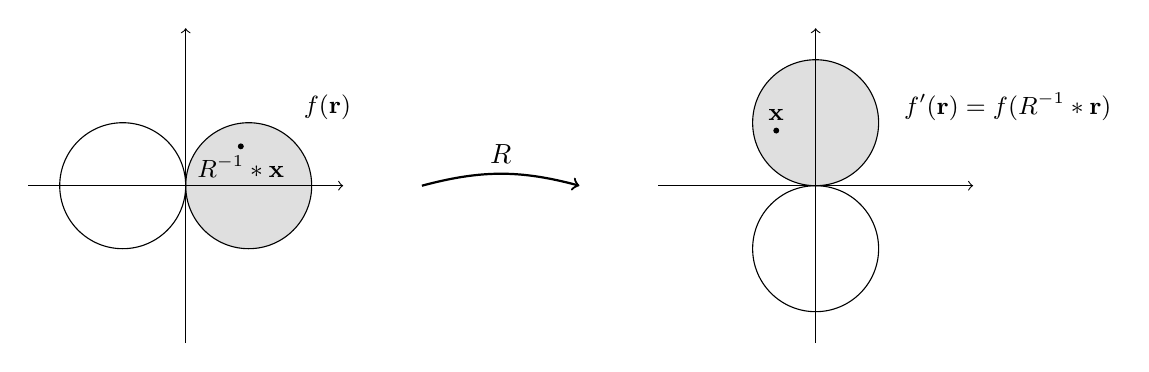
\begin{tikzpicture}
            \draw[fill=gray!25] (0.8,0) circle (0.8);
            \draw (-0.8,0) circle (0.8);
            \node at (1.8,1){\small\(f(\vb{r})\)};
            \draw[->] (-2,0)--(2,0);
            \draw[->] (0,-2)--(0,2);
            \draw[fill=black] (0.7,0.5)node[below]{\small\(R^{-1}*\vb{x}\)} circle (0.03);

            \draw[->,thick] (3,0)to[bend left=15]node[above]{\(R\)}(5,0);

            \draw[fill=gray!25] (8,0.8) circle (0.8);
            \draw (8,-0.8) circle (0.8);
            \node at (9,1)[right]{\small\(f'(\vb{r})=f(R^{-1}*\vb{r})\)};
            \draw[->] (6,0)--(10,0);
            \draw[->] (8,-2)--(8,2);
            \draw[fill=black] (7.5,0.7)node[above]{\small\(\vb{x}\)} circle (0.03);
        \end{tikzpicture}
        \caption{Acting a group element on a function.}
    \end{figure}
    When talking about a function, what we do is to associate a value to each point in the space. When we act the group element to the function, what we do is the change the associated value to a different place. For example, if the value of a function \(f\) is \(f(\vb{r})\) at some position \(\vb{r}\). Then if we act a group element \(R\) on the function, the value \(f(\vb{r})\) will now be associated to a new position \(R*\vb{r}\). Therefore, if we call the function after the group action \(f'(\vb{r})\coloneqq R*f(\vb{r})\), then we have \(f'(R*\vb{r})=f(\vb{r})\). We can rewrite this as
    \begin{equation}
        R*f(\vb{r})=f'(\vb{r})=f(R^{-1}*\vb{r})\,.
    \end{equation}
    
    For example, to construct another representation of the \(C_3\) group, we can attach one \(s\) orbital to each of the vertex of an equilateral triangle. Then under the symmetry operations of the triangle, the three \(s\) orbitals transform to each other, so we can use the three \(s\) orbitals as a basis
    \begin{equation}
        \begin{pmatrix}
            s_A & s_B & s_C
        \end{pmatrix}\,.
    \end{equation}
    \begin{figure}[ht!]
        \centering
        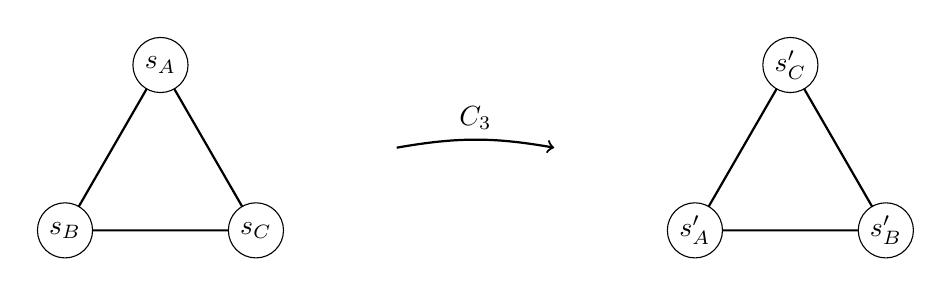
\begin{tikzpicture}
            \node at (0,0){\tikz[scale=0.7]{
                \draw[thick] (0,2)--(1.732,-1)--(-1.732,-1)--(0,2);
                \draw[fill=white] (0,2) node{\(s_A\)} circle (0.5);
                \draw[fill=white] (1.732,-1) node{\(s_C\)} circle (0.5);
                \draw[fill=white] (-1.732,-1) node{\(s_B\)} circle (0.5);
            }};
            \draw[thick,->] (3,0)to[bend left=10]node[above]{\(C_3\)} (5,0);
            \node at (8,0){\tikz[scale=0.7]{
                \draw[thick] (0,2)--(1.732,-1)--(-1.732,-1)--(0,2);
                \draw[fill=white] (0,2) node{\(s_C'\)} circle (0.5);
                \draw[fill=white] (1.732,-1) node{\(s_B'\)} circle (0.5);
                \draw[fill=white] (-1.732,-1) node{\(s_A'\)} circle (0.5);
            }};
        \end{tikzpicture}
    \end{figure}

    Then, for example, since we have
    \begin{equation}
        C_3*s_A=s_B\,,\ C_3*s_B=s_C\,,\ C_3*s_C=s_A\,,
    \end{equation}
    the representation of \(C_3\) in this basis will be
    \begin{equation}
        \DD(C_3)=\begin{pmatrix}
            0 & 0 & 1 \\
            1 & 0 & 0 \\
            0 & 1 & 0
        \end{pmatrix}\,.
    \end{equation}

    In general, the \(n\)-dimensional representation matrix \(D(R)\) of a symmetry operator \(R\) in a properly chosen basis \((\varphi_1,\varphi_2,\dots,\varphi_n)\) is defined by the equation
    \begin{equation}
        R*\varphi_i=\sum_j\varphi_j D_{ji}(R)\,.
    \end{equation}
    A representation constructed this way is guaranteed to be a homomorphism since
    \begin{align}
        R*(S*\varphi_i)&=R*\varphi_j D_{ji}(S)\notag \\
        &=\varphi_k D_{kj}(R)D_{ji}(S)
    \end{align}
    (summation convention applies), and by compatibility,
    \begin{align}
        R*(S*\varphi_i)&=(R\cdot S)*\varphi_i\notag \\
        &=\varphi_k D_{ki}(RS)\,,
    \end{align}
    and therefore we have a homomorphism
    \begin{equation}
        \DD(R)\DD(S)=\DD(RS)\,.
    \end{equation}

    From the homomorphism condition, we can see that for any representation \(\DD\) of the group \(G\),
    \begin{equation}
        \DD(R)=\DD(ER)=\DD(E)\DD(R)=\II\DD(R)\,,
    \end{equation}
    so the representation of the identity element is always the identity matrix, and
    \begin{equation}
        \DD(E)=\DD(R)\DD(R^{-1})=\II\,,
    \end{equation}
    so \(\DD(R^{-1})=(\DD(R))^{-1}\) for all \(R\in G\).

    \subsection{Equivalence}
    Let \((\vu{\imath}, \vu{\jmath}, \vu{k})\) be a basis of a three dimensional vector space, and \(\vb{v}\) be some vector with coordinates \((x,y,z)\) in this basis. Then
    \begin{equation}
        \vb{v}=\begin{pmatrix}
            \vu{\imath} & \vu{\jmath} & \vu{k}
        \end{pmatrix}\begin{pmatrix}
            x \\ y \\ z
        \end{pmatrix}\,.
    \end{equation}
    Let \(\TT\) be any invertible matrix, then we have \(\TT\TT^{-1}=\II\), and so we also have
    \begin{equation}
        \vb{v}=\begin{pmatrix}
            \vu{\imath} & \vu{\jmath} & \vu{k}
        \end{pmatrix}\begin{pmatrix}
            x \\ y \\ z
        \end{pmatrix}=\begin{pmatrix}
            \vu{\imath} & \vu{\jmath} & \vu{k}
        \end{pmatrix}\TT\TT^{-1}\begin{pmatrix}
            x \\ y \\ z
        \end{pmatrix}=\begin{pmatrix}
            \vu{\imath}' & \vu{\jmath}' & \vu{k}'
        \end{pmatrix}\begin{pmatrix}
            x' \\ y' \\ z'
        \end{pmatrix}\,,
    \end{equation}
    where
    \begin{equation}
        \begin{pmatrix}
            \vu{\imath}' & \vu{\jmath}' & \vu{k}'
        \end{pmatrix}=\begin{pmatrix}
            \vu{\imath} & \vu{\jmath} & \vu{k}
        \end{pmatrix}\TT\,,\ \begin{pmatrix}
            x' \\ y' \\ z'
        \end{pmatrix}=\TT^{-1}\begin{pmatrix}
            x \\ y \\ z
        \end{pmatrix}
    \end{equation}
    are a transformed basis and transformed coordinates of exactly the same vector in this transformed basis.

    We can do the same thing to transform a basis we used to construct a representation, and see what happens to the representation matrix. Let the action of \(R\) on a vector \(\vb{v}\) give
    \begin{equation}
        R*\vb{v}=\begin{pmatrix}
            \vu{\imath} & \vu{\jmath} & \vu{k}
        \end{pmatrix}\DD(R)\begin{pmatrix}
            x \\ y \\ z
        \end{pmatrix}\,,
    \end{equation}
    then we can also write
    \begin{align}
        R*\vb{v}&=\begin{pmatrix}
            \vu{\imath} & \vu{\jmath} & \vu{k}
        \end{pmatrix}\TT\TT^{-1}\DD(R)\TT\TT^{-1}\begin{pmatrix}
            x \\ y \\ z
        \end{pmatrix}\notag \\
        &=\begin{pmatrix}
            \vu{\imath}' & \vu{\jmath}' & \vu{k}'
        \end{pmatrix}\DD(R)'\begin{pmatrix}
            x' \\ y' \\ z'
        \end{pmatrix}\,.
    \end{align}
    This time, in the transformed basis, the representation of \(R\) is given by
    \begin{equation}
        \DD(R)'=\TT^{-1}\DD(R)\TT\,.
    \end{equation}
    We call this type of transformations on a representation matrix \textit{similarity} or \textit{equivalence} transformation, and the two representation \(\DD\) and \(\DD'\) are said to be \textit{equivalent}. Crucially, there is nothing fundamentally different between two equivalent representations --- they have just used two different set of basis vectors that represents the same vector space.

    \begin{ex}
        Let's consider a \(\mathrm{BF_3}\) molecule, whose full symmetry is given by the \(D_{3h}\) group. For simplicity, we will use it to representation of a smaller group \(D_3\), which is a subgroup of \(D_{3h}\).
        \begin{figure}[ht!]
            \centering
            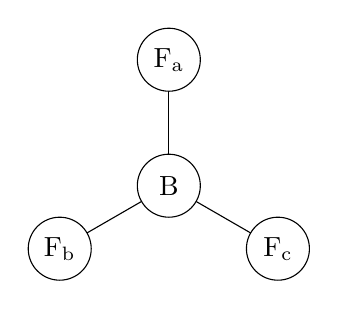
\begin{tikzpicture}[scale=0.8]
                \draw (0,0)--+(90:2);
                \draw (0,0)--+(-30:2);
                \draw (0,0)--+(210:2);
                \draw[fill=white] (0,0)node{\(\mathrm{B}\)} circle (0.5);
                \draw[fill=white] (0,2)node{\(\mathrm{F_a}\)} circle (0.5);
                \draw[fill=white] (1.732,-1)node{\(\mathrm{F_c}\)} circle (0.5);
                \draw[fill=white] (-1.732,-1)node{\(\mathrm{F_b}\)} circle (0.5);
            \end{tikzpicture}
        \end{figure}


        \begin{table}[ht!]
            \centering\small
            \begin{tabular}{ccccccc}
                \toprule
                ~ & \(E\) & \(C_3\) & \(C_3^2\) & \(C_2^a\) & \(C_2^b\) & \(C_2^c\) \\ \midrule
                \((s)\) & \((1)\) & \((1)\) & \((1)\) & \((1)\) & \((1)\) & \((1)\) \\
                \((p_z)\) & \((1)\) & \((1)\) & \((1)\) & \((-1)\) & \((-1)\) & \((-1)\) \\
                \((p_x,p_y)\) & \(\begin{pmatrix}
                    1 & 0 \\ 0 & 1
                \end{pmatrix}\) & \(\begin{pmatrix}
                    -\frac{1}{2} & -\frac{\sqrt{3}}{2} \\ \frac{\sqrt{3}}{2} & -\frac{1}{2}
                \end{pmatrix}\) & \(\begin{pmatrix}
                    -\frac{1}{2} & \frac{\sqrt{3}}{2} \\ -\frac{\sqrt{3}}{2} & -\frac{1}{2}
                \end{pmatrix}\) & \(\begin{pmatrix}
                    1 & 0 \\ 0 & -1
                \end{pmatrix}\) & \(\begin{pmatrix}
                    -\frac{1}{2} & -\frac{\sqrt{3}}{2} \\ -\frac{\sqrt{3}}{2} & \frac{1}{2}
                \end{pmatrix}\) & \(\begin{pmatrix}
                    -\frac{1}{2} & \frac{\sqrt{3}}{2} \\ \frac{\sqrt{3}}{2} & \frac{1}{2}
                \end{pmatrix}\) \\
                \((p_1,p_{-1})\) & \(\begin{pmatrix}
                    1 & 0 \\ 0 & 1
                \end{pmatrix}\) & \(\begin{pmatrix}
                    \omega^* & 0 \\ 0 & \omega
                \end{pmatrix}\) & \(\begin{pmatrix}
                    \omega & 0 \\ 0 & \omega^*
                \end{pmatrix}\) & \(\begin{pmatrix}
                    0 & -1 \\ -1 & 0
                \end{pmatrix}\) & \(\begin{pmatrix}
                    0 & -\omega \\ -\omega^* & 0
                \end{pmatrix}\) & \(\begin{pmatrix}
                    0 & -\omega^* \\ -\omega & 0
                \end{pmatrix}\) \\
                \((s_a,s_b,s_c)\) & \(\begin{pmatrix}
                    1 & 0 & 0 \\ 0 & 1 & 0 \\ 0 & 0 & 1
                \end{pmatrix}\) & \(\begin{pmatrix}
                    0 & 0 & 1 \\ 1 & 0 & 0 \\ 0 & 1 & 0
                \end{pmatrix}\) & \(\begin{pmatrix}
                    0 & 1 & 0 \\ 0 & 0 & 1 \\ 1 & 0 & 0
                \end{pmatrix}\) & \(\begin{pmatrix}
                    1 & 0 & 0 \\ 0 & 0 & 1 \\ 0 & 1 & 0
                \end{pmatrix}\) & \(\begin{pmatrix}
                    0 & 0 & 1 \\ 0 & 1 & 0 \\ 1 & 0 & 0
                \end{pmatrix}\) & \(\begin{pmatrix}
                    0 & 1 & 0 \\ 1 & 0 & 0 \\ 0 & 0 & 1
                \end{pmatrix}\) \\ \bottomrule
            \end{tabular}
        \end{table}
        
        The basis functions are atomic orbitals of \(\mathrm{BF_3}\). \(s_a\), \(s_b\) and \(s_c\) are the fluorine \(2s\) orbitals and the rest are boron orbitals. The functions \(p_{1}\) and \(p_{-1}\) are the complex \(p\) orbitals (that are eigenfunctions of \(\hat{L}_z\) operators) defined by
        \begin{equation}
            p_{1}=-\frac{1}{\sqrt{2}}(p_x+\ii p_y)\qquad p_{-1}=\frac{1}{\sqrt{2}}(p_x-\ii p_y)\,.
        \end{equation}\
        \(\omega\) is the third root of unity
        \begin{equation}
            \omega=\exp\left(\frac{2\pi \ii}{3}\right)=-\frac{1}{2}+\frac{\sqrt{3}}{2}\ii\,.
        \end{equation}

        From the definition of the complex \(p_{\pm 1}\) orbitals, we can see that they span the same vector space as the \((p_x,p_y)\) basis functions, and so these two representations should be equivalent. We have
        \begin{equation}
            \begin{pmatrix}
                p_1 & p_{-1}
            \end{pmatrix}=\begin{pmatrix}
                p_x & p_y
            \end{pmatrix}\TT=\begin{pmatrix}
                p_x & p_y
            \end{pmatrix}\begin{pmatrix}
                -\frac{1}{\sqrt{2}} & \frac{1}{\sqrt{2}} \\
                -\frac{\ii}{\sqrt{2}} & -\frac{\ii}{\sqrt{2}}
            \end{pmatrix}\,.
        \end{equation}
        You can check that these two rows of representation matrices are related by
        \begin{equation}
            \DD^{\pm 1}(R)=\TT^{-1}\DD^{xy}(R)\TT\,.
        \end{equation}
    \end{ex}

    \subsection{Reducibility}
    In the example above, we formed a one-dimensional representation of \(D_3\) using the basis set \((p_z)\) and a two-dimensional representation using \((p_x,p_y)\). There is nothing stopping us to construct a three-dimensional representation using the combined basis set \((p_x,p_y,p_z)\). However, all the operations in \(D_3\) will leave the \(p_x,p_y\) orbitals into a linear combination of themselves, and leave \(p_z\) either unchanged or merely change its sign. The two vector subspaces spanned by \((p_x,p_y)\) and \((p_z)\) do not mix --- that's why we are able to form representations using these two basis sets at the beginning. We call these two space, \(\spn(p_x,p_y)\) and \(\spn(p_z)\), the \textit{invariant subspaces} of the whole vector space \(\spn(p_x,p_y,p_z)\). Then if we use this three dimensional basis set to form a representation, it will look like this.
    \begin{align}
        \DD^{xyz}(E)&=\begin{pNiceMatrix}[margin]
			\Block[borders={top,bottom,right,left,tikz=dashed}]{2-2}{}
			1 & 0 & 0 \\
            0 & 1 & 0 \\
            0 & 0 & \Block[borders={top,bottom,right,left,tikz=dashed}]{1-1}{} 1
		\end{pNiceMatrix} & \DD^{xyz}(C_3)&=\begin{pNiceMatrix}[margin]
			\Block[borders={top,bottom,right,left,tikz=dashed}]{2-2}{}
			-\frac{1}{2} & -\frac{\sqrt{3}}{2} & 0 \\
            \frac{\sqrt{3}}{2} & -\frac{1}{2} & 0 \\
            0 & 0 & \Block[borders={top,bottom,right,left,tikz=dashed}]{1-1}{} 1
		\end{pNiceMatrix} \notag\\
        \DD^{xyz}(C_3^2)&=\begin{pNiceMatrix}[margin]
			\Block[borders={top,bottom,right,left,tikz=dashed}]{2-2}{}
			-\frac{1}{2} & \frac{\sqrt{3}}{2} & 0 \\
            -\frac{\sqrt{3}}{2} & -\frac{1}{2} & 0 \\
            0 & 0 & \Block[borders={top,bottom,right,left,tikz=dashed}]{1-1}{} 1
		\end{pNiceMatrix} & \DD^{xyz}(C_2^a)&=\begin{pNiceMatrix}[margin]
			\Block[borders={top,bottom,right,left,tikz=dashed}]{2-2}{}
			1 & 0 & 0 \\
            0 & -1 & 0 \\
            0 & 0 & \Block[borders={top,bottom,right,left,tikz=dashed}]{1-1}{} -1
		\end{pNiceMatrix} \notag\\
        \DD^{xyz}(C_3)&=\begin{pNiceMatrix}[margin]
			\Block[borders={top,bottom,right,left,tikz=dashed}]{2-2}{}
			-\frac{1}{2} & -\frac{\sqrt{3}}{2} & 0 \\
            -\frac{\sqrt{3}}{2} & \frac{1}{2} & 0 \\
            0 & 0 & \Block[borders={top,bottom,right,left,tikz=dashed}]{1-1}{} -1
		\end{pNiceMatrix} & \DD^{xyz}(C_3^2)&=\begin{pNiceMatrix}[margin]
			\Block[borders={top,bottom,right,left,tikz=dashed}]{2-2}{}
			-\frac{1}{2} & \frac{\sqrt{3}}{2} & 0 \\
            \frac{\sqrt{3}}{2} & \frac{1}{2} & 0 \\
            0 & 0 & \Block[borders={top,bottom,right,left,tikz=dashed}]{1-1}{} -1
		\end{pNiceMatrix}\,.
    \end{align}
    All these representations are in the block diagonal form, where the two blocks are the two smaller representations formed by \((p_x,p_y)\) and \((p_z)\).
    \begin{equation}
        \DD^{xyz}=\begin{pNiceMatrix}[margin]
            \Block[borders={top,bottom,right,left,tikz=dashed}]{2-2}{}
            \Block{2-2}{\DD^{xy}} & & \\
             & & \\
             & & \Block[borders={top,bottom,right,left,tikz=dashed}]{1-1} {\DD^z}
        \end{pNiceMatrix}\,.
    \end{equation}
    There are no off-block-diagonal elements since as we just claimed before, the two vector subspaces do not mix. For the representations that can be written in the block diagonal form, we say it is a \textit{direct sum} of its diagonal-block representations, written
    \begin{equation}
        \DD^{xyz}=\DD^{xy}\oplus\DD^{z}\,.
    \end{equation}
    This definition can be extended to define direct sums of multiple representations.

    Some representations themselves are not in the block diagonal form, but they are equivalent to the direct sum of the direct sum of smaller representations. Let's consider the example above again. This time, we define a new basis set
    \begin{equation}
        \begin{aligned}
            \varphi_1&=\sqrt{\frac{1}{3}}(s_a+s_b+s_c) \\
            \varphi_2&=\sqrt{\frac{1}{6}}(2s_a-s_b-s_c) \\
            \varphi_3&=\sqrt{\frac{1}{2}}(s_b-s_c)\,.
        \end{aligned}
    \end{equation}
    This is a transformation of the \((s_a,s_b,s_c)\) basis
    \begin{equation}
        \begin{pmatrix}
            \varphi_1 & \varphi_2 & \varphi_3
        \end{pmatrix}=\begin{pmatrix}
            s_a & s_b & s_c
        \end{pmatrix}\begin{pmatrix}
            \sqrt{\frac{1}{3}} & \sqrt{\frac{2}{3}} & 0 \\
            \sqrt{\frac{1}{3}} & -\sqrt{\frac{1}{6}} & \sqrt{\frac{1}{2}} \\
            \sqrt{\frac{1}{3}} & -\sqrt{\frac{1}{6}} & -\sqrt{\frac{1}{2}}
        \end{pmatrix}\,,
    \end{equation}
    and so in this new basis, the representation matrices are
    \begin{align}
        \DD^{\varphi}(E)&=\begin{pNiceMatrix}[margin]
            \Block[borders={top,bottom,right,left,tikz=dashed}]{1-1}{} 1 & 0 & 0 \\
			0 & \Block[borders={top,bottom,right,left,tikz=dashed}]{2-2}{} 1 & 0 \\
            0 & 0 & 1 
		\end{pNiceMatrix} & \DD^{\varphi}(C_3)&=\begin{pNiceMatrix}[margin]
			\Block[borders={top,bottom,right,left,tikz=dashed}]{1-1}{} 1 & 0 & 0 \\
			0 & \Block[borders={top,bottom,right,left,tikz=dashed}]{2-2}{} -\frac{1}{2} & -\frac{\sqrt{3}}{2}\\
            0 & \frac{\sqrt{3}}{2} & -\frac{1}{2}
		\end{pNiceMatrix} \notag\\
        \DD^{\varphi}(C_3^2)&=\begin{pNiceMatrix}[margin]
			\Block[borders={top,bottom,right,left,tikz=dashed}]{1-1}{} 1 & 0 & 0 \\
			0 & \Block[borders={top,bottom,right,left,tikz=dashed}]{2-2}{} -\frac{1}{2} & \frac{\sqrt{3}}{2}\\
            0 & -\frac{\sqrt{3}}{2} & -\frac{1}{2}
		\end{pNiceMatrix} & \DD^{\varphi}(C_2^a)&=\begin{pNiceMatrix}[margin]
			\Block[borders={top,bottom,right,left,tikz=dashed}]{1-1}{} 1 & 0 & 0 \\
			0 & \Block[borders={top,bottom,right,left,tikz=dashed}]{2-2}{} 1 & 0 \\
            0 & 0 & -1
		\end{pNiceMatrix} \notag\\
        \DD^{\varphi}(C_3)&=\begin{pNiceMatrix}[margin]
			\Block[borders={top,bottom,right,left,tikz=dashed}]{1-1}{} 1 & 0 & 0 \\
			0 & \Block[borders={top,bottom,right,left,tikz=dashed}]{2-2}{} -\frac{1}{2} & -\frac{\sqrt{3}}{2} \\
            0 & -\frac{\sqrt{3}}{2} & \frac{1}{2}
		\end{pNiceMatrix} & \DD^{\varphi}(C_3^2)&=\begin{pNiceMatrix}[margin]
			\Block[borders={top,bottom,right,left,tikz=dashed}]{1-1}{} 1 & 0 & 0 \\
			0 & \Block[borders={top,bottom,right,left,tikz=dashed}]{2-2}{} -\frac{1}{2} & \frac{\sqrt{3}}{2} \\
            0 & \frac{\sqrt{3}}{2} & \frac{1}{2}
		\end{pNiceMatrix}\,.
    \end{align}
    This time the representation is again in a direct sum form, with
    \begin{equation}
        \DD^{\varphi}=\DD^{\mathrm{B},s}\oplus\DD^{xy}\,,
    \end{equation}
    and hence the representation formed by fluorine \(s\) orbitals is equivalent to the direct sum of \(\DD^{B,s}\) and \(\DD^{xy}\), written
    \begin{equation}
        \DD^{\mathrm{F},s}\sim\DD^{\mathrm{B},s}\oplus\DD^{xy}\,.
    \end{equation}
    
    If a representation is equivalent to a direct sum of some lower-dimensional representation, then we say this representation is \textit{reducible}. On the other hand, there are some representations that cannot be reduced in this way (the one dimensional trivial representation is clearly an example). These representations are \textit{irreducible}. The irreducible representations of a group have their canonical names, which you can find in the character table of the group (although we have not introduced what is a character table yet).
    
    Any representation of a group can be reduced into a number of irreducible representations of the group (by finding a suitable basis in which this matrix is block diagonal) so we can always write
    \begin{equation}
        \Gamma\sim\bigoplus_{i=1}^{N}m_i\Gamma^{i}\,,
    \end{equation}
    where \(\{\Gamma^{i}\}_{i=1}^{N}\) are the inequivalent irreducible representations of the group, and the multiplicity \(m_i\) is the time a certain irreducible representation \(\Gamma^{i}\) appear on the diagonal blocks. However, in practice, we often just write it as
    \begin{equation}
        \Gamma=\bigoplus_{i=1}^{N}m_i\Gamma^{i}
    \end{equation}
    since we don't usually distinguish between equivalent matrices.

    However, it is not straight forward at all to figure out under what basis is our representation block diagonal, making it seem very difficult to reduce a representation. Next, we will introduce a powerful concept called \textit{character}, which is, as its name suggests, characteristic of a representation and allows us to reduce a representation easily.

    \newpage
    \section{Characters}
    \subsection{Characters}
    Representations are nice and intuitive, but they are just not the nicest thing to work with. Matrices are large, and it is tedious to manipulate them. More crucially, two equivalent representations, which are fundamentally the same thing, may look completely different after a similarity transform. Is there a nicer thing that is invariant under the transformation of a basis?

    The key is the trace.

    \begin{defn}
        The \textit{characters} of a representation \(\Gamma\) are the traces of the representation matrices, denoted \(\chi\).
    \end{defn}
    \begin{prop}
        Let \(\DD,\TT\) be \(n\times n\) matrices with \(\TT\) invertible. Then
        \begin{equation}
            \tr(\DD)=\tr(\TT^{-1}\DD\TT)\,.
        \end{equation}
    \end{prop}
    \begin{proof}
        \begin{align}
            \tr(\TT^{-1}\DD\TT)&=(\TT^{-1})_{ij}D_{jk}T_{ki}\notag\\
            &=T_{ki}(\TT^{-1})_{ij}D_{jk}\notag\\
            &=\delta_{kj}D_{jk}\notag\\
            &=D_{jj}=\tr(\DD)\,.
        \end{align}\qed
    \end{proof}
    This has two immediate consequences. First, if two representations are equivalent, then their characters are the same. This is obvious. Second, if \(R,S\in G\) are in the same conjugacy class (say, \(R=QSQ^{-1}\)), then their characters under the same representation are the same. This is because by the homomorphism requirement,
    \begin{align}
        \DD(R)&=\DD(QSQ^{-1})\notag\\
        &=\DD(Q)\DD(S)\DD(Q^{-1})\notag\\
        &=\DD(Q)\DD(S)\DD(Q)^{-1}\,,
    \end{align}
    so their traces are equal.
    
    This allows us to construct a so-called \textit{character table} to list the characters of all the inequivalent irreducible representations of a group,\footnote{For a finite group, there are necessarily finitely many irreducible representations, so the table can be listed --- we will show this later.} in which the rows are the different inequivalent irreducible representations and the columns are the character classes (Remember the characters of the elements in the same class are equal, so we can list them in the same column). For example, for the \(D_3\) group, we will get something like this.
    \begin{table}[ht!]
        \centering
        \begin{tabular}{lccc}
            \toprule & \(E\) & \(2C_3\) & \(3C_2\) \\ \midrule
            \(A_1\) & \(1\) & \(1\) & \(1\) \\
            \(A_2\) & \(1\) & \(1\) & \(-1\) \\
            \(E\) & \(2\) & \(-1\) & \(0\) \\ \bottomrule
        \end{tabular}
    \end{table}

    Moreover, since the trace is a sum of the diagonal elements, it is clear that the character of a reducible matrix is the character of its components. That is, if
    \begin{equation}
        \Gamma=\bigoplus_{i=1}^{N}m_i\Gamma^{i}\,,
    \end{equation}
    then
    \begin{equation}
        \chi=\sum_{i=1}^{N}m_i\chi^{i}\,.
    \end{equation}
    Then, to figure out the component of a reducible representation \(\Gamma\), we only need to work out the characters of what irreducible representations (which are listed in the character table) sum to it. This still seems to be a difficult task to do if we have a large number of irreducible representations. But luckily, we have the orthogonality theorems!
    
    \subsection{Orthogonality Theorems}
    Now we will introduce one of the most powerful theorems in representation theory, upon which many useful results are derived.

    \begin{thm}[Great orthogonality theorem]
        Let \(\{\Gamma^{a}\}\) be the set of inequivalent irreducible unitary representations of a finite group \(G\), then
        \begin{equation}
            \sum_{R\in G}D_{ip}^{a}(R)^* D_{jq}^{b}(R)=\frac{\abs{G}}{n_a}\delta_{ab}\delta_{ij}\delta_{pq}\,.
        \end{equation}
        where \(n_a\) is the dimension of \(\Gamma^a\).\footnote{We requested the irreducible representations in \(\{\Gamma^{a}\}\) to be inequivalent to avoid the case that \(\Gamma^a\sim\Gamma^b\) but \(\Gamma^a\ne\Gamma^b\) --- a formula does exist for such case, but it is more complicated. We are not proving this theorem here. A proof of this, along with a more expanded and rigorous treatment of groups and representations can be found in my notes on NST Part IB Mathematical Methods. It spends half a chapter to arrive at this result, so it is too large to fit in the margin, or even in the appendix.}
    \end{thm}

    This is an extremely powerful result, as can be seen by the three Kronecker deltas --- you need to sum over the same element of the same irreducible representation, otherwise you will get a zero. This great orthogonality theorem allows us to show some useful properties of the characters.

    \begin{thm}[First orthogonality theorem]
        Let \(\{\chi^a\}\) be the characters of the inequivalent irreducible representations \(\{\Gamma^a\}\) of a finite group \(G\).
        \begin{equation}
            \sum_{R\in G}\chi^a(R)^*\chi^b(R)=\abs{G}\delta_{ab}\,.
        \end{equation}
    \end{thm}
    \begin{proof}
        \begin{align}
            \sum_{R}\chi^a(R)^*\chi^b(R)&=\sum_{R}\sum_{i,k}D_{ii}^{a}(R)^*D_{kk}^{b}(R)\notag\\
            &=\sum_{i,k}\frac{\abs{G}}{n_a}\delta_{ab}\delta_{ik}\delta_{ik}\notag\\
            &=\abs{G}\delta_{ab}\,.
        \end{align}\qed
    \end{proof}

    This is also known as row orthogonality, because what it says is that the rows of a character table are orthogonal. To see this, we need to rewrite it a little bit. In a character table, we group the group elements in the same conjugacy class together into the same column since their characters are the same. We can use this to simplify our sum. Instead of summing over all the elements in the group, we can sum over the conjugacy classes, provided that we remember to multiply the number of elements in the conjugacy class.

    \begin{cor}[Row orthogonality]
        \begin{equation}
            \sum_c h_c\chi^a(c)^*\chi^b(c)=\abs{G}\delta_{ab}\,,
        \end{equation}
        where \(h_c\) is the size of the conjugacy class \(c\).
    \end{cor}

    If we view each row of a character table as the entries of a vector, what this means is that these vectors are orthonormal under some slightly modified version of the dot product where we have an additional factor:\footnote{If you have learned some linear algebra before, you should notice that this is the metric of the inner product.}
    \begin{equation}
        \vb{a}\vdot\vb{b}=\sum_{i}\frac{h_i}{\abs{G}}a_i^*b_i\,.
    \end{equation}
    This then allows us to conveniently reduce a reducible representation! Suppose we have a vector space spanned by orthonormal basis \((\vb{e}_1,\vb{e}_2,\dots,\vb{e}_n)\), and we want to find out the components of a vector \(\vb{v}\), i.e. to find out the coefficients \(c_1,c_2,\dots,c_n\) such that
    \begin{equation}
        \vb{v}=\sum_{i=1}^{n}c_i\vb{e}_i\,.
    \end{equation}
    What we can do is to take the dot product of \(\vb{v}\) with each of the basis vector \(\vb{e}_j\) and we would obtain the coefficient \(c_j\).
    \begin{align}
        \vb{e}_j\vdot\vb{v}&=\sum_{i=1}^{n}c_i\vb{e}_j\vdot\vb{e}_i\notag\\
        &=\sum_{i=1}^{n}c_i\delta_{ij}=c_j\,.
    \end{align}
    We can do exactly the same thing here, as long as we remember to use our slightly modified version of the dot product.

    \begin{thm}[Reduction formula]
        Let \(\{\chi^{a}\}_{a=1}^{n}\) be the characters of the inequivalent irreducible representations \(\{\Gamma^a\}_{a=1}^{n}\) of a finite group \(G\), and \(\Gamma\) is a reducible representation with character \(\chi\), then \(\Gamma\) is reduced to
        \begin{equation}
            \Gamma=\bigoplus_{a=1}^{n}m_a\Gamma^a
        \end{equation}
        with
        \begin{equation}
            m_a=\frac{1}{\abs{G}}\sum_c h_c\chi^{a}(c)^*\chi(c)\,,
        \end{equation}
        where \(h_c\) is the number of elements of conjugacy class \(c\).
    \end{thm}
    \begin{proof}
        We use the row orthogonality.
        \begin{align}
            \frac{1}{\abs{G}}\sum_c h_c\chi^a(c)^*\chi(c)&=\frac{1}{\abs{G}}\sum_c h_c\chi^a(c)^*\sum_i m_i\chi^i(c)\notag\\
            &=\sum_i m_i\delta_{ia}\notag\\
            &=m_a\,.
        \end{align}\qed
    \end{proof}

    What's even nicer about the character table is that the columns of it are also orthogonal! This is the second orthogonality theorem, also known as column orthogonality.
    \begin{thm}[Second orthogonality theorem (column orthogonality)]
        Let \(\{\chi^a\}\) be the characters of the inequivalent irreducible representations \(\{\Gamma^a\}\) of a finite group \(G\).
        \begin{equation}\label{column_orthogonality}
            \sum_{a}\chi^a(c)^*\chi^a(c')=\frac{\abs{G}}{h_c}\delta_{cc'}\,.
        \end{equation}
    \end{thm}
    This is, however, much harder to prove and we will not prove it. The row orthogonality and column orthogonality combined leads to a very nice result.
    \begin{cor}[Character table is square]
        Let \(G\) be a finite group, then the number of inequivalent irreducible representations of \(G\) and the number of conjugacy classes of \(G\) are equal.
    \end{cor}
    \begin{proof}
        Let \(\{c_i\}_{i=1}^{p}\) be the conjugacy classes and \(\{\Gamma^a\}_{a=1}^{m}\) be the inequivalent irreducible representations, i.e. there are \(p\) conjugacy classes and \(m\) inequivalent irreducible representations.
        
        Each row has \(p\) entries, so we can view each row as a vector in \(\CC^p\), and by row orthogonality these vectors are orthonormal. These \(m\) linearly independent vectors in \(\CC^p\) must span a subspace \(\CC^m\le\CC^p\), so \(m\le p\). Similarly, column orthogonality means that viewing each column as a vector in \(\CC^m\), these vectors are also orthonormal. These are \(p\) linearly independent vectors in \(\CC^m\), so they must span a subspace \(\CC^p\le\CC^m\), so \(p\le m\). \(m=p\).\qed
    \end{proof}
    \begin{cor}
        Let \(\{\Gamma^a\}\) be the inequivalent irreducible representations of a finite group \(G\), then
        \begin{equation}
            \sum_a n_a^2=\abs{G}\,,
        \end{equation}
        where \(n_a\) is the dimension of \(\Gamma^a\).
    \end{cor}
    \begin{proof}
        Put \(c=c'=\{E\}\), the class of the identity element in the column orthogonality theorem (\ref{column_orthogonality}).\qed
    \end{proof}

    \begin{ex}
        Consider again the representation of \(D_3\) group spanned by the three fluorine \(s\) orbital in \(\mathrm{BF_3}\). Last time we have shown that under the basis transformation
        \begin{equation}
            \begin{aligned}
                \varphi_1&=\sqrt{\frac{1}{3}}(s_a+s_b+s_c) \\
                \varphi_2&=\sqrt{\frac{1}{6}}(2s_a-s_b-s_c) \\
                \varphi_3&=\sqrt{\frac{1}{2}}(s_b-s_c)\,,
            \end{aligned}
        \end{equation}
        this reducible representation becomes a direct sum
        \begin{equation}
            \Gamma=A_1\oplus E\,.
        \end{equation}
        
        But finding the suitable basis transformation matrix out of nowhere to block-diagonalise the representation matrix seems like a difficult thing to do. Now, using the reduction formula, we can directly reduce a representation without doing so. To use the reduction formula, we only need to find the character of our representation spanned by \((s_a,s_b,s_c)\). This is simple --- the character is the sum of the diagonal element of a representation matrix, and a diagonal element of a representation matrix means how much has a basis transformed into itself after the group action. For example, to work out the character of \(C_2^a\), we need to find
        \begin{equation}
            \chi(C_2^a)=D_{11}(C_2^a)+D_{22}(C_2^a)+D_{33}(C_2^a)\,.
        \end{equation}
        \(D_{11}(C_2^a)\) is the \(s_a\) component of \(s_a\) after the action of \(C_2^a\); \(s_a\) is not moved by \(C_2^a\) so this is one. \(D_{22}(C_2^a)\) is the \(s_b\) component of \(s_b\) after the action of \(C_2^a\), while \(s_b\) is moved to \(s_c\) after \(C_2^a\) so this is zero, meaning \(s_b'=C_2^a*s_b\) has no component of \(s_b\). Similarly, \(s_c'=C_2^a*s_c\) has no component of \(s_c\), so \(D_{33}(C_2^a)=0\). Summing these up, we get \(\chi(C_2^a)=1+0+0=1\). Now since the three \(C_2\) elements are in the same conjugacy class, their characters are \(1\) as well. Doing this for all other character classes, we find that the characters of our representation is        
        \begin{table}[H]
            \centering
            \begin{tabular}{ccccccc}
                \toprule
                ~ & \(E\) & \(2C_3\) & \(3C_2\) \\ \midrule
                \(\chi\) & \(3\) & \(0\) & \(1\) \\ \toprule
            \end{tabular}
        \end{table}

        Now to reduce this representation, we need the character table.
        \begin{table}[ht!]
            \centering
            \begin{tabular}{ccccccc}
                \toprule
                ~ & \(E\) & \(2C_3\) & \(3C_2\) \\ \midrule
                \(A_1\) & \(1\) & \(1\) & \(1\) \\
                \(A_2\) & \(1\) & \(1\) & \(-1\) \\
                \(E\) & \(2\) & \(-1\) & \(0\) \\ \bottomrule
            \end{tabular}
        \end{table}

        Now we can use the reduction formula to compute the multiplicities.
        \begin{align}
            m_{A_1}&=\frac{1}{\abs{G}}\sum_{c}h_c\chi^{A_1}(c)^*\chi(c)=\frac{1}{6}(1\times 1\times 3+2\times 1\times 0+3\times 1\times 1)=1\\
            m_{A_2}&=\frac{1}{\abs{G}}\sum_{c}h_c\chi^{A_2}(c)^*\chi(c)=\frac{1}{6}(1\times 1\times 3+2\times 1\times 0+3\times (-1)\times 1)=0\\
            m_{E}&=\frac{1}{\abs{G}}\sum_{c}h_c\chi^{E}(c)^*\chi(c)=\frac{1}{6}(1\times 2\times 3+2\times (-1)\times 0+3\times 0\times 1)=1\,,
        \end{align}
        and hence we have successfully reduced out representation:
        \begin{equation}
            \Gamma=A_1\oplus E\,.
        \end{equation}
    \end{ex}

    \subsection{Projection Formula and Gram--Schmidt Orthogonalisation}
    Now we can successfully reduce a representation without finding the basis transformation matrix that block-diagonalises the representation matrix, but it actually turns out that this transformation matrix is a rather useful thing, and we want to know it in the most cases. For example, if we know that after the transformation
    \begin{equation}
        \begin{aligned}\label{BF3_SO}
            \varphi_1&=\sqrt{\frac{1}{3}}(s_a+s_b+s_c) \\
            \varphi_2&=\sqrt{\frac{1}{6}}(2s_a-s_b-s_c) \\
            \varphi_3&=\sqrt{\frac{1}{2}}(s_b-s_c)\,,
        \end{aligned}
    \end{equation}
    the representation becomes block diagonalised to
    \begin{equation}
        \Gamma^{\varphi}=\begin{pNiceMatrix}[margin]
            \Block[borders={top,bottom,right,left,tikz=dashed}]{1-1}{}\Block{1-1}{A_1} & & \\
			 & \Block[borders={top,bottom,right,left,tikz=dashed}]{2-2}{} \Block{2-2}{E} & \\
             & & \\
		\end{pNiceMatrix}\,,
    \end{equation}
    then this means that \((\varphi_1)\) itself spans \(A_1\), and \((\varphi_2,\varphi_3)\) together transforms as \(E\). This is known as the \textit{symmetry orbitals} --- the linear combination of atomic orbitals that transform as a specific irreducible representation. They are extremely useful in molecular orbital theories since, as you have seen in Part IB \textit{Symmetry and Bonding} course, only orbitals that transforms as the same irreducible representations have non-zero interactions. Therefore, knowing how to construct these orbitals would greatly reduce our workload when constructing molecular orbitals.

    Luckily, this is not difficult to do as long as we know to what irreducible representations our representation reduces to. Let's consider the following operator
    \begin{equation}
        \hat{P}_i^{a}\coloneqq\frac{n_a}{\abs{G}}\sum_{R\in G}D_{ii}^{a}(R)^* R\,,
    \end{equation}
    which is a particular linear combination of group elements, and see how it acts on a vector \(\vb{v}_j^{b}=\sum_k (v_j^b)_k\vb{e}_k\), represented in the basis \((\vb{e}_1,\vb{e}_2,\dots)\), that transforms as the \(j^{\text{th}}\) component of the irreducible representation \(\Gamma^{b}\). We have
    \begin{align}
        \hat{P}_i^a * \vb{v}_j^{b}&=\frac{n_a}{\abs{G}}\sum_{R}D_{ii}^{a}(R)^* R * \vb{v}_j^b \notag\\
        &=\frac{n_a}{\abs{G}}\sum_{R}D_{ii}^{a}(R)^*\sum_k (\vb{v}_j^b)_k\vb{e}_k D_{kj}^{b}(R) \notag\\
        &=\sum_{k} \delta_{ab}\delta_{ik}\delta_{ij} (\vb{v}_j^b)_k\vb{e}_k \notag\\
        &=\begin{cases}
            \sum_{k}(\vb{v}_i^a)_k\vb{e}_k=\vb{v}_i^{a} & \text{if }a=b,i=j \\
            0 & \text{otherwise,}
        \end{cases}
    \end{align}
    This is exactly what defines a \textit{projection operator}! If you act \(\hat{P}_i^{a}\) on any vector, you will only get the component of it that transforms as the \(i\) component of the irreducible representation \(\Gamma^a\), and anything else will be annihilated, i.e. it projects a vector onto \(\vb{v}_i^a\).

    Theoretically, we can use this to obtain each component of an irreducible representation by acting the projection operators on arbitrary vectors, but this would require us to know the irreducible representations. What we usually have is only the character of the irreducible representations. What we can do is to sum up the components of the projection operators of the same irreducible representations, and define
    \begin{equation}
        \hat{P}^a\coloneqq\sum_{i=1}^{n_a}\hat{P}_i^{a}=\frac{n_a}{\abs{G}}\sum_R\chi^a(R)^* R\,.
    \end{equation}
    Now when you act this on an arbitrary vector, you will obtain the sum of its projection on all the components of an irreducible representation
    \begin{equation}
        \hat{P}^a * \vb{v}=\sum_{i=1}^{n_a}\hat{P}_i^a * \vb{v}=\sum_{i}\vb{v}_i^{a}\,.
    \end{equation}
    This could be troublesome for an irreducible representation that is not one-dimensional. For example, in the \(\mathrm{BF_3}\) example, if you act \(\hat{P}^{E}=\hat{P}_1^{E}+\hat{P}_2^{E}\) on an arbitrary vector, you will get a linear combination of \(\varphi_2\) and \(\varphi_3\), the two components that together transform as \(E\).

    Of course, we can directly use this mixture as one of the components of \(E\), since this is only a basis transformation of \(E\) and you will still get something equivalent to \(E\), which is still an \(E\) --- but we still need to get the other orthogonal components of the basis transforming as \(E\). This is done by a process called \textit{Gram--Schmidt orthogonalisation}. Let \(\vb{v}_1\) be the vector that we obtained from the projection operator, which we use as the vector that transforms as the first component of an irreducible representation \(\Gamma\) with dimension greater than 1. \(\Gamma\) is clearly not the totally symmetric representation (since its dimension is not 1), so there must be an operator \(R\) that acts on \(\vb{v}_1\) to generate some vector \(\vb{v}'=R*\vb{v}_1\) that is not completely aligned with \(\vb{v}_1\). Since \(\vb{v}_1\) in the basis set that generates \(\Gamma\), it will only be transformed into a sum of different components that transform as \(\Gamma\). Therefore, if \(\vb{v}'=R * \vb{v}_1\) has some component orthogonal to \(\vb{v}_1\), then this can be seen as a vector that transforms as the second component of \(\Gamma\). To extract this, we first normalise \(\vb{v}_1\) and \(\vb{v}'\), and then let
    \begin{equation}
        \vb{v}_2=\vb{v}'-(\vb{v}'\vdot\vb{v}_1)\vb{v}_1
    \end{equation}
    to get rid of any component of \(\vb{v}'\) that is aligned with \(\vb{v}_1\). This \(\vb{v}_2\) might be unnormalised, so we can normalise it, and we then get a \(\vb{v}_2\) that is orthonormal with \(\vb{v}_1\). We can repeat this process until we have generated all components of the basis that transforms as \(\Gamma\).

    \begin{ex}
        Back to the example of using the fluorine \(\mathrm{F}\) orbitals in \(\mathrm{BF_3}\) to represent \(D_3\) group. We know that the representation is \(\Gamma=A_1+E\), and let's find out the symmetry orbitals.
        
        First the \(A_1\) orbitals. This should be easy. We just pick any vector and act the projection operator of \(A_1\),
        \begin{align}
            \hat{P}^{A_1}&=\frac{n_{A_1}}{\abs{D_3}}\sum_{R\in D_3}\chi^{A_1}(R)^* R\notag\\
            &=\frac{1}{6}(E+C_3+C_3^2+C_2^a+C_2^b+C_2^c)\,,
        \end{align}
        onto it. The simplest choice of vector is one of the basis vectors. We would use \(s_a\) and we get
        \begin{equation}
            \hat{P}^{A_1}*s_a=\frac{1}{6}(s_a+s_b+s_c+s_a+s_c+s_b)=\frac{1}{3}(s_a+s_b+s_c)\,.
        \end{equation}
        This can be normalised to get the \(A_1\) symmetry orbital
        \begin{equation}
            \phi_{A_1}=\frac{1}{\sqrt{3}}(s_a+s_b+s_c)\,.
        \end{equation}

        Next, let's calculate the \(E\) symmetry orbitals. This should be a little more difficult. Let's first construct the projection operator.
        \begin{align}
            \hat{P}^{E}&=\frac{n_{E}}{\abs{D_3}}\sum_{R\in D_3}\chi^{E}(R)^* R\notag\\
            &=\frac{1}{3}(2E-C_3-C_3^2)\,.
        \end{align}
        We act this on \(s_a\) to get
        \begin{equation}
            \hat{P}^{E}*s_a=\frac{1}{3}(2s_a-s_b-s_c)\,.
        \end{equation}
        We can normalise this to get the first \(E\) symmetry orbital
        \begin{equation}
            \phi_{E,1}=\frac{1}{\sqrt{6}}(2s_a-s_b-s_c)\,.
        \end{equation}
        Next, let's construct the second \(E\) symmetry orbital by Gram--Schmidt orthogonalisation. We act some arbitrary group element onto our first symmetry orbital that does not leave it unchanged. \(C_3\) seems to be a good choice.
        \begin{equation}
            \phi'=C_3*\phi_{E,1}=\frac{1}{\sqrt{6}}(2s_b-s_c-s_a)\,.
        \end{equation}
        We subtract the \(\phi_{E,1}\) component from it and get
        \begin{align}
            \phi'-(\phi'\vdot \phi_{E,1})\phi_{E,1}&=\frac{1}{\sqrt{6}}(2s_b-s_c-s_a)-\frac{1}{6}(-2-2+1)\frac{1}{\sqrt{6}}(2s_a-s_b-s_c)\notag\\
            &=\frac{3}{2\sqrt{6}}(s_b-s_c)\,.
        \end{align}
        This can be normalised to get the second symmetry orbital of \(E\):
        \begin{equation}
            \phi_{E,2}=\frac{1}{\sqrt{2}}(s_b-s_c)\,.
        \end{equation}
        You can check that these are identical to what we asserted in (\ref{BF3_SO}). 
    \end{ex}

    \newpage
    \section{Rotation Group and Spherical Harmonics}
    In the first chapter, we have shown that for a molecular system, rotation is a symmetry operation. We can therefore consider the group of all 3D rotations about any axis that leaves an origin unchanged (that is the centre of mass for a molecular system), known as the \textit{full rotation group}. We can denote its elements by \(R(\vb{u})\), where \(\vb{u}=\alpha\vu{u}\), \(\alpha=\norm{\vb{u}}\) is the angle of rotation, and \(\vu{u}\) is the unit vector along the rotation axis. Mathematically, the full rotation group is exactly the \textit{special orthogonal group of order 3}, the group of \(3\times 3\) orthogonal matrices with determinant \(+1\), denoted \(\SO(3)\). There is a one-to-one correspondence between rotation operations \(R\) and matrices \(\mathsf{R}\in\SO(3)\) --- they are isomorphic, so we see them as the same group.

    We have claimed before that the theory of the \(\SO(3)\) group is deeply linked to the theory of angular momentum. This can be seen from Noether's theorem, which says the rotational symmetry leads to the conservation of angular momentum. Also, if we consider the rotation \(\mathsf{R}\in\SO(3)\) of a function \(\psi(\vb{r})\) in 3D space (for example the wavefunction), then the function after rotation, denoted \(\psi'(\vb{r})\), satisfies
    \begin{equation}
        \psi'(\vb{r})=\psi(\mathsf{R}^{-1}\vb{r})\,.
    \end{equation}
    More explicitly, if we identify the axis of rotation as the \(z\) axis, and we rotate by an angle \(\alpha\), then the value of the rotated function now at \((r,\theta,\varphi)\) would be the value of the function originally at \((r,\theta,\varphi-\alpha)\). We can construct an operator
    \begin{equation}\label{J_generates_rotation}
        \hat{J}_z=i\hbar\lim_{\alpha\to 0}\frac{R(\alpha\vu{z})-E}{\alpha}
    \end{equation}
    which captures the effect of an infinitesimal rotation about \(z\) axis (the \(i\hbar\) here is just a matter of convention). This is known as the \textit{generator} of the rotation. Then its effect on some function \(\psi\) is
    \begin{equation}
        \hat{J}_z\psi(r,\theta,\varphi)=i\hbar\lim_{\alpha\to 0}\frac{\psi(r,\theta,\varphi-\alpha)-\psi(r,\theta,\varphi)}{\alpha}=-i\hbar\pdv{\psi}{\varphi}\,.
    \end{equation}
    This is exactly the \(z\) component of the angular momentum operator! We say angular momentum \textit{generates} the rotation.

    The properties of rotations give hints on the properties of angular momentum operators. For systems governed by Hamiltonians with rotational symmetries, since rotation is a symmetry action, the angular momentum operator commutes with the Hamiltonian operator: \([\hat{H},\hat{\vb{J}}]=0\). However, rotations along different axes do not commute. You can try it! Find an object, rotate it \(90^\circ\) along the \(x\) axis, then \(90^\circ\) along \(z\) axis, and you will find that it is different if you first rotate it \(90^\circ\) along \(z\) axis then along \(x\) axis --- the order of rotations matters. Hence the different components of the angular momentum operators do not commute. However, the rotations along the same axis commute. Therefore we have \([\hat{J}_i,\hat{J}_j]\ne 0\) for \(i\ne j\), while \([\hat{J}_i,\hat{J}_i]=0\).
    
    A quick aside, if you run the same process above for spatial translation, you will find that the momentum operator \(\hat{\vb{P}}\) is the generator of spatial translation. Rotating an object followed by a translation is not the same as translating the object followed by a rotation (because the object is now off the origin), unless the direction of translation and the axis of rotation is the same (then the object is still on the rotation axis), so we have \([\hat{J}_i,\hat{P}_j]\ne 0\) for \(i\ne j\), while \([\hat{J}_i,\hat{P}_i]=0\). More specifically, since momentum is a vector, it \textit{transforms as a vector} under rotation, so
    \begin{equation}
        [\hat{J}_i,\hat{P}_j]=i\hbar\sum_k\epsilon_{ijk} \hat{P}_k\,.
    \end{equation}
    The position operator \(\hat{\vb{X}}\) is also a vector, so it also transforms as a vector under rotation
    \begin{equation}
        [\hat{J}_i,\hat{X}_j]=i\hbar\sum_k\epsilon_{ijk} \hat{X}_k\,.
    \end{equation}
    However, translations in different directions commute: translation along \(x\) by \(1\unit{m}\) then along \(y\) by \(2\unit{m}\) is the same as first translating along \(y\) by \(2\unit{m}\) then along \(x\) by \(1\unit{m}\) --- the order does not matter. Therefore, all components of translation commute with each other
    \begin{equation}
        [\hat{P}_i,\hat{P}_j]=0\,.
    \end{equation}
    Reporting your coordinate does not affect anything, so components of the position operator commute
    \begin{equation}
        [\hat{X}_i,\hat{X}_j]=0\,.
    \end{equation}
    Finally, asking where you are and then move away is not the same as first move away then ask where you are, unless the component of the position coordinate you are asking is orthogonal to the direction you are moving, so
    \begin{equation}
        [\hat{X}_i,\hat{P}_j]=i\hbar\delta_{ij}\,.
    \end{equation}
    The idea of generators allows us to understand the commutation relations of operators in a simple and intuitive way.

    Next, we will quote, without proof, some properties of the \(\SO(3)\) group and its representations. The theoretical details are far beyond the scope of our course.
    \begin{enumerate}[topsep=0pt,label=(\roman*)]
        \item The rotation \(R(\alpha\vu{u})\) through an angle \(\alpha\) about an axis \(\vu{u}\) is in the same class as a rotation \(R(\alpha'\vu{u}')\) if and only if \(\alpha=\alpha'\). The class of \(\SO(3)\) contains all rotations through the same angle \(\alpha\) about any axis.
        \item The irreducible representations of \(\SO(3)\) are labelled by the quantum number \(J\) of angular momentum. Representation \(\Gamma^{J}\) has dimension \(2J+1\).
        \item The spherical harmonics \(Y_{JM}\) are the basis functions for the representation \(\Gamma^{J}\).\footnote{We will not prove this. This is exactly the last result in the Mathematical Tripos Part II \textit{Representation Theory} course so it is impossible to cover this in a 6-lecture chemistry course. However, we can briefly justify this. The angular momentum operator generates a rotation, so an infinitesimal rotation \(R(\delta\alpha\vu{z})\) is represented by
        \begin{equation}
            E-\frac{\ii}{\hbar}\delta\alpha\hat{J_z}
        \end{equation}
        by reverting the expression (\ref{J_generates_rotation}). Then a rotation of non-infinitesimal degree \(\alpha\) can be obtained by repeatedly acting the infinitesimal rotations by \(\alpha/N\) for \(N\to\infty\) times:
        \begin{equation}
            R(\alpha\vu{z})=\lim_{N\to\infty}\left(1-\frac{\ii\alpha}{\hbar N}\hat{J}_z\right)^N=\ee^{-\ii\alpha\hat{J}_z/\hbar}\,.
        \end{equation}
        This allows us to use the eigenstates of the angular momentum operator (spherical harmonics) as the basis, which are labelled by \(\ket{J,M}\), with
        \begin{align}
            \hat{\vb{J}}^2\ket{J,M}=\hbar^2 J(J+1)\ket{J,M}\\
            \hat{J}_z\ket{J,M}=\hbar M\ket{J,M}\,.
        \end{align}
        For any value of \(J\), \(M_J\in\{-J,-J+1,\dots,J\}\), so there are \(2J+1\) of them. \(\{\ket{J,M}\}_{M=-J}^{J}\) is therefore a \(2J+1\) dimensional basis, and rotation along the \(z\) axis acting on them by
        \begin{equation}
            R(\alpha\hat{z})*\ket{J,M}=\ee^{-\ii\alpha\hat{J}_z/\hbar}\ket{J,M}=\ee^{-\ii M\alpha}\ket{J,M}\,.
        \end{equation}
        For this to be a homomorphism, we require \(R(2\pi\hat{z})\) to be mapped to the identity, so we must have \(\ee^{-2\pi\ii M}=1\). This is true if and only if \(M\) is an integer, which is true if and only if \(J\) is an integer. Hence, these representations are \(2J+1\) dimensional with \(J\) an integer, and the basis functions are the spherical harmonics. However, we haven't shown that they are exactly the irreducible ones. Moreover, there are some subtle details with those half-integer \(J\) states. Roughly speaking, the half-integer \(J\) states form the \textit{projective representations}, when you consider all states \(\lambda\ket{\psi}\), \(\lambda\in\CC\) to be the same as \(\ket{\psi}\) as in quantum mechanics, and those particles with half-integer spin values (internal \(J\) value) are known as the \textit{spinors}. For example, when \(J=\frac{1}{2}\) and \(M=\pm\frac{1}{2}\), you can see \(\ee^{-\ii M\alpha}\) returns to \(1\) when \(\alpha=720^\circ\)! You will need to rotate an electron (\(s=\frac{1}{2}\)) by \(720^\circ\) for it to go back to its original state!}
    \end{enumerate}


    We can then work out the character of the irreducible representations of \(\SO(3)\). The spherical harmonics are
    \begin{equation}
        Y_{JM}(\theta,\varphi)=C_{JM}P_{J}^{\abs{M}}(\cos\theta)\ee^{\ii M\varphi}\,,
    \end{equation}
    where \(P_J^{\abs{M}}\) is the \textit{associated Legendre polynomial}. Since the rotations of the same angle about any axis are in the same conjugacy class, they have the same character, so it is the easiest to consider the rotation about the \(z\) axis. We have
    \begin{equation}
        R(\alpha\vu{z})*Y_{JM}=Y_{JM}(\theta,\varphi-\alpha)=\ee^{-\ii M\alpha}Y_{JM}\,,
    \end{equation}
    so the \(M^{\text{th}}\) diagonal component of the irreducible representation \(\Gamma^{J}\) is
    \begin{equation}
        D_{MM}^{J}(\alpha)=\ee^{-\ii M\alpha}\,.
    \end{equation}
    The character is then
    \begin{align}
        \chi^{J}(\alpha)&=\sum_{M=-J}^{J}\ee^{-\ii M\alpha}\notag\\
        &=\frac{\ee^{\ii J\alpha}[1-\ee^{-\ii(2J+1)\alpha}]}{1-\ee^{-\ii \alpha}}\notag\\
        &=\frac{\sin(J+\frac{1}{2})\alpha}{\sin\frac{1}{2}\alpha}\,.
    \end{align}
    \begin{ex}
        Suppose we are interested in the characters of the \(\mathrm{f}\) orbitals in the \(T_d\) point group, and we cannot find them in our standard character table. We can work them out easily using the formula above.

        The \(\mathrm{f}\) functions are exactly the spherical harmonics with \(J=3\). There are 7 of them, so the character of \(E\) is 7. For \(C_3\), it is a rotation of \(\frac{2\pi}{3}\), so
        \begin{equation}
            \chi(C_3)=\frac{\sin\frac{7}{2}\frac{2\pi}{3}}{\sin\frac{1}{2}\frac{2\pi}{3}}=1\,.
        \end{equation}
        For \(C_2\), which is a rotation by \(\pi\), the character is
        \begin{equation}
            \chi(C_2)=\frac{\sin\frac{7}{2}\pi}{\sin\frac{1}{2}\pi}=-1\,.
        \end{equation}
        Next, we have \(S_4=iC_4\). Since \(\mathrm{f}\) functions change their sign under inversion, \(\chi(S_4)=\chi(iC_4)=-\chi(C_4)\), and so
        \begin{equation}
            \chi(S_4)=-\frac{\sin\frac{7}{2}\frac{\pi}{2}}{\sin\frac{1}{2}\frac{\pi}{2}}=+1\,.
        \end{equation}
        Similarly, \(\sigma_d=iC_2\), so
        \begin{equation}
            \chi(\sigma_d)=-\chi(C_2)=+1\,.
        \end{equation}

        \begin{table}[ht!]
            \centering
            \begin{tabular}{cccccc}
                \toprule
                \(T_d\) & \(E\) & \(8C_3\) & \(3C_2\) & \(6S_4\) & \(6\sigma_d\) \\ \midrule
                7f & 7 & 1 & \(-1\) & 1 & 1 \\ \bottomrule
            \end{tabular}
        \end{table}
    \end{ex}

    \newpage
    \section{Totally Symmetric Representation and Direct Product Representations}
    \subsection{Totally Symmetric Representation}
    Every group has a special one-dimensional representation called the \textit{totally symmetric representation} (or \textit{trivial representation}), where the representation matrices of all elements are \((1)\) and the characters are all \(1\). It has different conventional notations in different groups (\(A_1,A_{1g},A_1',\Sigma_g^{+},S\) \textit{etc.}), but here we call it \(\Gamma^{(1)}\) for simplicity.

    If we use the totally symmetric representation \(\Gamma^{(1)}\) as one of the representations in the great orthogonality theorem, then we get a useful formula
    \begin{equation}\label{rep_sum_over_element}
        \frac{1}{\abs{G}}\sum_{R\in G}D_{ij}^{\Gamma}(R)=\begin{cases}
            0 & \text{if }\Gamma\ne \Gamma^{(1)} \\
            1 & \text{if }\Gamma=\Gamma^{(1)}\,,
        \end{cases}
    \end{equation}
    where both \(i\) and \(j\) are apparently forced to equal 1 in the totally symmetric case.

    Next, let's consider the behaviour of physical properties of molecules, such as charge or dipole moment. If a molecule belongs to a certain point group, then all the action of all the symmetry operations should, by definition, leave the appearance of the molecule unchanged, and so it cannot change the value of any physical quantity. Let's consider a physical quantity \(\mu\) of a molecule, the components of which span a representation \(\Gamma^\mu\). For example, if \(\vb{\mu}=(\mu_x,\mu_y,\mu_z)\) is a vector, then its three components will transform as vectors \(\vb{x}\), \(\vb{y}\) and \(\vb{z}\) (or equivalently as Cartesian functions \(x\), \(y\) and \(z\)) respectively, which spans a three dimensional representation. Then for any component of the quantity \(\mu_i\), the action of any symmetry operation \(R\) should leave it unchanged:
    \begin{equation}
        \mu_i=R*\mu_i=\sum_j\mu_j D_{ji}^\mu(R)\,.
    \end{equation}
    Then if we sum over the operations in the group, we get
    \begin{equation}
        \abs{G}\mu_i=\sum_{R\in G}R*\mu_i=\sum_{j}\mu_j\sum_{R}D_{ji}^\mu(R)\,.
    \end{equation}
    Then if \(\Gamma^\mu\) is irreducible, by (\ref{rep_sum_over_element}), we have \(\mu_i=0\) unless \(\Gamma^\mu=\Gamma^{(1)}\). On the other hand, if \(\Gamma^\mu=\Gamma^{(1)}\), then this equation is simply \(\mu_i=\mu_i\). It tells us nothing about this quantity --- it can take any value. If \(\Gamma^\mu\) is reducible, then we can reduce it and then apply it to each irreducible components of it. Only the components that transform as \(\Gamma^{(1)}\) can be non-zero.
    
    This leads to an important conclusion. The number of independent nonzero components of a physical quantity \(\mu\) is the number of times that the totally symmetric representation occurs in \(\Gamma^\mu\).

    \begin{ex}
        The polarisability \(\alpha\) is a rank 2 symmetric tensor describing the dipole moment of an object induced by an electric field
        \begin{equation}
            \mu_i=\sum_j\alpha_{ij}E_j\,,
        \end{equation}
        where \(i,j\in\{x,y,z\}\), and \(\alpha_{ij}=\alpha_{ji}\) by symmetry. It therefore has six independent components and the component \(\alpha_{ij}\) transforms like the quadratic Cartesian function \(ij\).

        The \(\mathrm{BF_3}\) molecule belongs to the \(D_{3h}\) point group, and the character table of \(D_{3h}\) tells us how the quadratic functions transform in \(D_{3h}\).
        \begin{table}[ht!]
            \centering
            \begin{tabular}{ccccc}
                \toprule
                Component & Cartesian function & Irrep & Conclusion \\ \midrule
                \(\alpha_{zz}\) & \(z^2\) & \(A_1'\) & \(\alpha_{zz}\ne 0\) \\
                \(\alpha_{xx}+\alpha_{yy}\) & \(x^2+y^2\) & \(A_1'\) & \(\alpha_{xx}+\alpha_{yy}\ne 0\) \\
                \(\begin{matrix}
                    \alpha_{xx}-\alpha_{yy} \\ \alpha_{xy}
                \end{matrix}\) & \(\begin{matrix}
                    x^2-y^2 \\ xy
                \end{matrix}\) & \(\Big\}\quad E'\quad\Big\{\) & \(\begin{matrix}
                    \alpha_{xx}-\alpha_{yy}=0 \\ \alpha_{xy}=0
                \end{matrix}\) \\
                \(\begin{matrix}
                    \alpha_{xz} \\ \alpha_{yz}
                \end{matrix}\) & \(\begin{matrix}
                    xz \\ yz
                \end{matrix}\) & \(\Big\}\quad E''\quad\Big\{\) & \(\begin{matrix}
                    \alpha_{xz}=0 \\ \alpha_{yz}=0
                \end{matrix}\) \\ \bottomrule
            \end{tabular}
            \caption{The components of polarisability tensor in \(D_{3h}\), the Cartesian function and hence the irreducible representation they transform as.}
        \end{table}

        The representation spanned by the polarisability components, \(\Gamma^{\alpha}\), has two \(A_1'\) components, and so the polarisability of \(\mathrm{BF_3}\) can only have two independent components: \(\alpha_{zz}=\alpha_{\parallel}\) and \(\alpha_{xx}=\alpha_{yy}=\alpha_{\perp}\).
    \end{ex}

    In quantum mechanics, we often encounter integrals, like \(\mel{\psi}{\hat{Q}}{\phi}=\int\dd{\tau}\psi^*\hat{Q}\phi\) which frequently arise in spectroscopy. We are often not particularly interested in the exact value of the integral --- we just want to know whether it is zero or not. Then symmetry can be a particularly useful argument.

    Let's consider a simple integral \(\int\dd{\tau}F_i^\Gamma\), whose integrand transform as the \(i^{\text{th}}\) component of the irreducible representation \(\Gamma\). The integral is over all space, so we can freely transform our integrand without affecting the value of the Integral
    \begin{equation}
        \abs{G}\int\dd{\tau} F_i^\Gamma=\sum_{R\in G}\int\dd{\tau}R*F_i^\Gamma=\sum_{R\in G}\int\dd{\tau}F_j^{\Gamma}D_{ji}(R)\,,
    \end{equation}
    where \(F_j^{\Gamma}\) is the corresponding function transforming as the \(j^{\text{th}}\) component of \(\Gamma\). Then by (\ref{rep_sum_over_element}),
    \begin{equation}
        \sum_{R\in G}D_{ji}(R)=0
    \end{equation}
    unless \(\Gamma\) is the totally symmetric representation. Hence, we conclude that an integral can be non-zero only if the integrand transforms as the totally symmetric representation.

    However, if the integrand is a product of functions and operators, like in \(\int\dd{\tau}\psi^*\hat{Q}\phi\), where each function and operator transform as some representation on their own, we need to work out how their product transforms. To do this, we need the direct product representation.

    \subsection{Direct Product Representation}
    Suppose we have an \(m\)-dimensional representation \(\Gamma^{a}\) generated by a basis \((\vb{u}_1,\dots,\vb{u}_m)\) and an \(n\)-dimensional representation \(\Gamma^b\) generated by a basis \((\vb{v}_1,\dots,\vb{v}_n)\). We can define a \textit{direct product basis}, \(\{\vb{u}_i\otimes\vb{v}_j\}_{i=1}^{m}{}_{j=1}^{n}\) composed of \(mn\) `combined basis vectors' composed of one basis taken from each basis set. We can then use this to define the \textit{direct product representation}\footnote{More formally in pure mathematics, they are known as the \textit{tensor product representations} as they are representations on the tensor product spaces. So in more formal representation theories, all those `direct products' should be replaced by \textit{tensor products} as tensor products has more algebraic structures than the direct product that we have assumed throughout our calculations below. The tensor product can be thought of as the direct product, but with the following few extra equivalence relations imposed (mathematically, this is called taking a quotient)
    \begin{equation}
        (v,w)+(v',w)\sim(v+v',w)\,,\; (v,w)+(v,w')\sim(v,w+w')\text{ and } c(v,w)\sim(cv,w)\sim(v,cw)\,.
    \end{equation}
    See more details in \cref{Appendix:Tensor}. However, this is a chemistry course so we will stick to chemists' conventions and call them direct products.}, \(\Gamma^{a}\otimes\Gamma^{b}\), defined by the action
    \begin{align}
        R*(\vb{u}_i\otimes\vb{v}_j)&\coloneqq(R*\vb{u}_i)\otimes(R*\vb{v}_j)=\left(\sum_{k=1}^{m}\vb{u}_k D_{ki}^{a}(R)\right)\otimes\left(\sum_{l=1}^{n}\vb{v}_l D_{lj}^{b}(R)\right)\notag\\
        &=\sum_{k=1}^{m}\sum_{l=1}^{n}\vb{u}_k\otimes\vb{v}_l D_{ki}^{a}(R) D_{lj}^{b}(R)\notag\\
        &\eqqcolon \sum_{(k,l)=(1,1)}^{(m,n)}\vb{u}_k\otimes\vb{v}_l D_{(k,l),(i,j)}^{\Gamma^{a}\otimes\Gamma^{b}}(R)\,,
    \end{align}
    and so
    \begin{equation}
        D_{(k,l),(i,j)}^{\Gamma^{a}\otimes\Gamma^{b}}\coloneqq D_{ki}^{a}(R) D_{lj}^{b}(R)\,.
    \end{equation}
    The resulting representation is \(mn\) dimensional, for which both the indices of the rows and the columns run from \((1,1)\) to \((m,n)\). Of course, you have the freedom to relabel them as a single number from \(1\) to \(mn\).

    We can also find the character of the direct product representation
    \begin{align}
        \chi^{\Gamma^{a}\otimes\Gamma^{b}}(R)&=\sum_{(k,l)=(1,1)}^{(m,n)}\sum_{(i,j)=(1,1)}^{(m,n)}\delta_{ki}\delta_{lj} D_{(k,l),(i,j)}^{\Gamma^{a}\otimes\Gamma^{b}}\notag\\
        &=\sum_{i,j} D_{ii}^{a}(R) D_{jj}^{b}(R)\notag\\
        &=\chi^{a}(R)\chi^{b}(R)\,.
    \end{align}
    The character of a direct product is the product of the characters.

    \begin{prop}
        The direct product is distributive on direct sums.
        \begin{equation}
            (\Gamma^a\oplus\Gamma^b)\otimes(\Gamma^c\oplus\Gamma^d)=(\Gamma^a\otimes\Gamma^c)\oplus(\Gamma^a\otimes\Gamma^d)\oplus(\Gamma^b\otimes\Gamma^c)\oplus(\Gamma^b\otimes\Gamma^d)\,.
        \end{equation}
    \end{prop}
    \begin{rem}
        This allows us to take the direct product of reducible representations as well as the irreducible ones.
    \end{rem}
    \begin{proof}
        This is the easiest seen by examining the characters of both sides. The character of the left-hand side is
        \begin{equation}
            (\chi^a+\chi^b)\times(\chi^c+\chi^d)=\chi^a\chi^c+\chi^a\chi^d+\chi^b\chi^c+\chi^b\chi^d\,,
        \end{equation}
        which is exactly the character of the right hand side. The characters are the same so the representations are equivalent (up to a similarity transform) --- remember that the character uniquely determines the irreducible representation decomposition of a reducible representation.\qed
    \end{proof}

    Now let's consider how a group element act on a product of functions \(f(\vb{r})g(\vb{r})\equiv fg(\vb{r})\):
    \begin{align}
        R*(fg(\vb{r}))&=fg(R^{-1}*\vb{r})\notag\\
        &=f(R^{-1}*\vb{r})g(R^{-1}*\vb{r})\notag\\
        &=(R*f(\vb{r}))(R*g(\vb{r}))\,.
    \end{align}
    A symmetry operator \(R\) affects each function individually --- this is exactly how we defined the direct product representation. Therefore, if some functions \((\xi_1,\dots,\xi_m)\) transform as a representation \(\Gamma^{a}\) and some functions \((\eta_1,\dots,\eta_n)\) transform as a representation \(\Gamma^{b}\), then their products \(\{\xi_i\eta_j\}\) transforms as the direct product representation \(\Gamma^{a}\otimes\Gamma^{b}\).

    To be more explicit, suppose the representation spanned by the set of functions \(\{\xi_i\eta_j\}\) is \(\Gamma\), then the component of \(\xi_i\eta_j\) along \(\xi_i\eta_j\) after the action of \(R\) is
    \begin{align}
        D_{(i,j),(i,j)}(R)&=R*(\xi_i\eta_j)\vdot \xi_i\eta_j \notag\\
        &=(R*\xi_i\vdot \xi_i)(R*\eta_j\vdot\eta_j) \notag\\
        &=D_{ii}^{a}(R) D_{jj}^{b}(R)\,,
    \end{align}
    where \(\vdot\) is some sort of dot product such that \(\xi_i\vdot\xi_j=\eta_i\vdot\eta_j=\delta_{ij}\). The character of \(R\) is
    \begin{equation}
        \chi(R)=\sum_{(i,j)=(1,1)}^{(m,n)}D_{(i,j),(i,j)}(R)=\sum_{i,j}D_{ii}^{a}(R)D_{jj}^{b}(R)=\chi^a(R)\chi^b(R)\,.
    \end{equation}
    This is indeed the direct product representation.

    It is useful to know how many times the totally symmetric representation occurs in a direct product.
    \begin{prop}
        If \(\Gamma^a\) and \(\Gamma^b\) are irreducible, then the direct product \({\Gamma^a}^*\otimes\Gamma^b\) (formed by the basis \(\{\xi_i^*\eta_j\}\)) contains the totally symmetric representation once if \(\Gamma^a\sim\Gamma^b\), and otherwise not at all.
    \end{prop}
    \begin{proof}
        We use the reduction formula to find the multiplicity of \(\Gamma^{(1)}\) in the direct product representation.
        \begin{align}
            m_1&=\frac{1}{\abs{G}}\sum_c h_c\chi^{(1)}(c)^*\chi^{{\Gamma^a}^*\otimes\Gamma^b}\notag \\
            &=\frac{1}{\abs{G}}\sum_c h_c\chi^{a}(c)^*\chi^{b}(c) \notag \\
            &=\delta_{ab}\,.
        \end{align}\qed
    \end{proof}

    It is also possible to work out such a symmetric component.
    \begin{prop}
        Suppose two bases \(\{\xi_i\}\) and \(\{\eta_j\}\) span two identical (not just equivalent) irreducible representations \(\Gamma^a=\Gamma^b=\Gamma\), then the symmetric component of a basis vector \(\xi_i^*\eta_j\) that transforms as the totally symmetric representation is
        \begin{equation}
            (\xi_i^*\eta_j)^{\Gamma^{(1)}}=\delta_{ij}\frac{1}{n_\Gamma}\sum_k\xi_k^*\eta_k\,.
        \end{equation}
    \end{prop}
    \begin{proof}
        We can project the direct product basis vector \(\xi_i^*\eta_j\) to \(\Gamma^{(1)}\).
        \begin{align}
            (\xi_i^*\eta_j)^{\Gamma^{(1)}}&=\frac{1}{\abs{G}}\sum_R D_{11}^{\Gamma^{(1)}}(R)R*(\xi_i^*\eta_j)\notag\\
            &=\frac{1}{\abs{G}}\sum_R\sum_{k,l}\xi_k^*\eta_l D_{ki}^{\Gamma}(R)^* D_{lj}^{\Gamma}(R)\notag\\
            &=\frac{1}{n_{\Gamma}}\sum_{k,l}\delta_{kl}\delta_{ij}\xi_k^*\eta_l\notag\\
            &=\delta_{ij}\frac{1}{n_{\Gamma}}\sum_k\xi_k^*\eta_k\,.
        \end{align}
        We can see that a basis function \(\xi_i^*\eta_j\) has a symmetric component if and only if \(i=j\). This is exactly the (unnormalised) function in the span of the direct product basis that transforms as the totally symmetric representation.\qed
    \end{proof}
    \begin{ex}
        For example, in the \(\mathrm{BF_3}\) molecule under \(D_3\),
        \begin{align}
            \xi_x&=\frac{1}{\sqrt{2}}(s_c-s_b)\notag\\
            \xi_y&=\frac{1}{\sqrt{6}}(2s_a-s_b-s_c)
        \end{align}
        transform as the \(x\) and \(y\) components of the \(E\) representation respectively. We also have
        \begin{align}
            \eta_x&=p_x\notag\\
            \eta_y&=p_y
        \end{align}
        transform as the \(x\) and \(y\) components of the \(E\) representation respectively. Then we know that
        \begin{equation}
            \xi_x^*\eta_x+\xi_y^*\eta_y
        \end{equation}
        transforms as the totally symmetric representation \(A_1\). If we, for any reason, want to work out the components of the boron \(p\) orbitals and the fluorine \(\mathrm{s}\) orbitals that give non-zero overlap integral, then this is the one.
    \end{ex}

    Let's wrap up. If \(\xi_i^a\) transforms as the component \(i\) of irreducible representation \(\Gamma^a\) and \(\eta_j^n\) transforms as the component \(j\) of the irreducible representation \(\Gamma^b\):
    \begin{itemize}[topsep=0pt]
        \item The overlap integral
        \begin{equation}
            \int\dd{\tau}{\xi_i^a}^*\eta_j^b=0
        \end{equation}
        unless \(\Gamma^a\sim\Gamma^b\).
        \item If \(\Gamma^a=\Gamma^b=\Gamma\) and \(i\ne j\), then
        \begin{equation}
            \int\dd{\tau}\xi_i^*\eta_j=0\,.
        \end{equation}
        \item If \(\Gamma^a=\Gamma^b=\Gamma\) and \(i=j\), then
        \begin{equation}
            \int\dd{\tau}\xi_i^*\eta_i=\frac{1}{n_\Gamma}\int\dd{\tau}\sum_k \xi_k^*\eta_k\,,
        \end{equation}
        which implies that the integral is the same for all \(i\).
    \end{itemize}
    If, in addition, we have an operator \(\hat{Q}_k^c\) transforming as the component \(k\) of the irreducible representation \(\Gamma^c\), then
    \begin{itemize}[topsep=0pt]
        \item The integral
        \begin{equation}
            \int\dd{\tau}{\xi_i^a}^*\hat{Q}_k^c\eta_j^b=0
        \end{equation}
        unless \(\Gamma^a\in\Gamma^b\otimes\Gamma^c\).
        \item The operator is totally symmetric e.g. the Hamiltonian, then
        \begin{equation}
            \int\dd{\tau}{\xi_i^a}^*\hat{Q}^{\Gamma^{(1)}}\eta_j^b=0
        \end{equation}
        unless \(\Gamma^a\sim\Gamma^b\).
        \item If the operator is totally symmetric and \(\Gamma^a=\Gamma^b=\Gamma\), then
        \begin{equation}
            \int\dd{\tau}\xi_i^*\hat{Q}^{\Gamma^{(1)}}\eta_j=0
        \end{equation}
        unless \(i=j\), in which case the result will be the same for all \(i\).
    \end{itemize}

    \subsection{The Symmetrised and Antisymmetrised Square}
    If we have two bases \((\xi_1,\dots,\xi_n)\) and \((\eta_i,\dots,\eta_n)\) spanning the same representation \(\Gamma\), then it turns out to be more useful to consider a transformed direct product basis, known as the \textit{symmetrised} and \textit{antisymmetrised square basis}. The \textit{symmetrised square basis} are functions of the form \(\{\xi_i\eta_j+\xi_j\eta_i\}\) that are symmetric with respect to the exchange of \(\eta\) and \(\xi\), and the \textit{antisymmetrised square basis} are those of the form \(\{\xi_i\eta_j-\xi_j\eta_i\}\) that are antisymmetric with respect to the exchange of \(\eta\) and \(\xi\).

    It turns out that the symmetrised basis transform only among themselves, and so they span a representation of dimension \(\frac{1}{2}n(n+1)\) called the \textit{symmetric square} of \(\Gamma\) and denoted \((\Gamma\otimes\Gamma)_+\). Similarly, the antisymmetrised square basis span a representation of dimension \(\frac{1}{2}n(n-1)\) called the \textit{antisymmetrised square}, denoted \((\Gamma\otimes\Gamma)_-\).\footnote{You can choose any distinct \(i\) and \(j\) to form a symmetric and antisymmetric basis vector --- these account for \(\frac{1}{2}n(n-1)\) of them each. In addition to that, symmetric basis can also have \(\xi_i\eta_i+\eta_i\xi_i\sim\xi_i\eta_i\), so the symmetric basis has \(n\) additional basis vectors of this type --- these would vanish for the antisymmetric case. The symmetric and antisymmetric basis sum up to \(n^2\) basis vectors as expected, as they are a basis transformation of the direct product basis so they should span the same vector space, and we should apparently have \(\Gamma\otimes\Gamma=(\Gamma\otimes\Gamma)_+\oplus(\Gamma\otimes\Gamma)_-\).}

    \begin{prop}
        The symmetrised and antisymmetrised square have characters
        \begin{equation}
            \chi^{(\Gamma\otimes\Gamma)_{\pm}}(R)=\frac{1}{2}[(\chi^\Gamma(R))^2\pm\chi^\Gamma(R^2)]\,.
        \end{equation}
    \end{prop}
    \begin{proof}
        Consider the action of \(R\) on the basis function \(\xi_i\eta_j\pm \xi_j\eta_i\).
        \begin{align}
            R*[\xi_i\eta_j\pm \xi_j\eta_i]&=\sum_{k,l}\xi_k D_{ki}^\Gamma(R)\eta_l D_{lj}^{\Gamma}(R) \pm \xi_k D_{kj}^\Gamma(R)\eta_l D_{li}^{\Gamma}(R) \notag \\
            &=\sum_{k,l} \xi_k\eta_l [D_{ki}^\Gamma(R) D_{lj}^{\Gamma}(R)\pm D_{kj}^\Gamma(R) D_{li}^{\Gamma}(R)]\,.\label{symm_action}
        \end{align}
        We have the freedom to relabel \(k\leftrightarrow l\) and so
        \begin{align}
            R*[\xi_i\eta_j\pm \xi_j\eta_i]&=\sum_{k,l}\xi_l\eta_k [D_{li}^\Gamma(R) D_{kj}^{\Gamma}(R)\pm D_{lj}^\Gamma(R) D_{ki}^{\Gamma}(R)] \notag \\
            &=\pm \sum_{k,l}\xi_l\eta_k [D_{ki}^\Gamma(R) D_{lj}^{\Gamma}(R) \pm D_{kj}^\Gamma(R) D_{li}^{\Gamma}(R)]\,.\label{symm_action_exchanged}
        \end{align}
        We can add (\ref{symm_action}) and (\ref{symm_action_exchanged}) to get
        \begin{align}
            R*[\xi_i\eta_j\pm \xi_j\eta_i]&=\frac{1}{2}\sum_{k,l}[\xi_k\eta_l\pm \xi_l\eta_k][D_{ki}^\Gamma(R) D_{lj}^{\Gamma}(R)\pm D_{kj}^\Gamma(R) D_{li}^{\Gamma}(R)] \notag\\
            &=\sum_{k,l}[\xi_k\eta_l\pm \xi_l\eta_k]\cdot D_{(k,l)(i,j)}(R)\,,
        \end{align}
        where the representation of \(R\) is
        \begin{equation}
            D_{(k,l)(i,j)}(R)=\frac{1}{2}[D_{ki}^\Gamma(R) D_{lj}^{\Gamma}(R)\pm D_{kj}^\Gamma(R) D_{li}^{\Gamma}(R)]\,.
        \end{equation}
        We can take its trace to get
        \begin{align}
            \chi^{(\Gamma\otimes\Gamma)_\pm}(R)&=\sum_{(k,l)=(i,j)}\frac{1}{2}[D_{ki}^\Gamma(R) D_{lj}^{\Gamma}(R)\pm D_{kj}^\Gamma(R) D_{li}^{\Gamma}(R)]\notag\\
            &=\frac{1}{2}\sum_{i,j}D_{ii}(R)D_{jj}(R)\pm D_{ij}(R)D_{ji}(R)\notag\\
            &=\frac{1}{2}[\chi(R)^2\pm\chi(R^2)]\,.
        \end{align}\qed
    \end{proof}

    It is possible to construct higher powers of a representation as well as their symmetrised and antisymmetrised parts, but they are in general of less interest. You will meet the symmetrised cube in one of the exercises.

    \begin{ex}
        If we have two sets of basis functions, \((\xi_x,\xi_y)\) and \((\eta_x,\eta_y)\), both transforming as the irreducible representation \(E\) in \(D_3\). Then the direct product basis is \((\xi_x\eta_x,\xi_x\eta_y,\xi_y\eta_x,\xi_y\eta_y)\), and the direct product transforms as \(E\otimes E=A_1\oplus A_2\oplus E\).

        We can transform this into symmetrised and antisymmetrised basis. The symmetrised basis is \((\xi_x\eta_x,\xi_y\eta_y,\xi_x\eta_y+\xi_y\eta_x)\) and the antisymmetrised basis is \((\xi_x\eta_y-\xi_y\eta_x)\). The symmetrised square is \((E\otimes E)_+=A_1\oplus E\), and the antisymmetrised square is \((E\otimes E)_-=A_2\). We can also work out the symmetry-adapted functions using the projection formula.
        \begin{table}[ht!]
            \centering
            \begin{tabular}{ccc}
                \toprule\renewcommand{\arraystretch}{1.2}
                \(A_1\): & \(\xi_x\eta_x+\xi_y\eta_y\) & symmetric \\
                \(A_2\): & \(\xi_x\eta_y-\xi_y\eta_x\) & antisymmetric \\
                \(E\): & \(\begin{matrix}
                    \xi_x\eta_y+\xi_y\eta_x \\
                    \xi_x\eta_x-\xi_y\eta_y
                \end{matrix}\) & symmetric \\ \bottomrule
            \end{tabular}
        \end{table}
    \end{ex}
    \subsection{Electronic Terms}
    An important application of this is in the electronic configuration of molecules. If we have two electrons in the same degenerate set of orbitals \(\{\psi_i\}\), then we can take the wavefunctions of the first electron as a basis \(\xi_i=\psi_i(\vb{r}_1)\) and the wavefunctions of the second electron as a basis \(\eta_i=\psi_i(\vb{r}_2)\). We can construct orbitally symmetric functions
    \begin{equation}
        \xi_i\eta_j+\xi_j\eta_i=\psi_i(\vb{r}_1)\psi_j(\vb{r}_2)+\psi_j(\vb{r}_1)\psi_i(\vb{r}_2)
    \end{equation}
    and orbitally antisymmetric ones
    \begin{equation}
        \xi_i\eta_j-\xi_j\eta_i=\psi_i(\vb{r}_1)\psi_j(\vb{r}_2)-\psi_j(\vb{r}_1)\psi_i(\vb{r}_2)\,.
    \end{equation}
    The orbitally symmetric ones, i.e. the components of the symmetrised square, are by construction symmetric with respect to the exchange of the electrons' spatial coordinates \(\vb{r}_1\leftrightarrow\vb{r}_2\), so by Pauli's principle, they have to be combined with antisymmetric (singlet) spin functions to maintain the overall antisymmetry of the electronic wavefunction. Similarly, the orbitally antisymmetric ones are the components of the antisymmetrised square, and should be combined with the symmetric (triplet) spin wavefunction.

    \begin{ex}
        In \(D_3\) group, we have
        \begin{equation}
            E\otimes E=A_1\oplus[A_2]\oplus E\,,
        \end{equation}
        where the antisymmetrised square is in square brackets. For an \(e^2\) configuration of a \(D_3\) molecule, with two electrons in a set of degenerate \(E\) orbitals. By the above argument, the allowed molecular terms are \(^1A_1\), \(^3A_2\) and \(^1E\), and \(^3A_2\) is the ground state by Hund's first rule.

        In \(O_h\) group,
        \begin{equation}
            T_{2g}\otimes T_{2g}=A_{1g}\oplus E_g\oplus[T_{1g}]\oplus T_{2g}\,,
        \end{equation}
        so the configuration \(t_{2g}^2\) leads to the molecular terms \(^1A_{1g}\), \(^1E_g\), \(^1T_{2g}\) and \(^3T_{1g}\), and the term \(^3T_{1g}\) is the lowest energy one.
    \end{ex}

    \subsubsection{Direct Product Representations of the Full Rotation Group}
    \begin{prop}[Clebsch--Gordan Rule]
        \begin{equation}
            \Gamma^{J_1}\otimes\Gamma^{J_2}=\Gamma^{J_1+J_2}\oplus\Gamma^{J_1+J_2-1}\oplus\dots\oplus\Gamma^{\abs{J_1-J_2}}\,.
        \end{equation}
    \end{prop}
    You will prove this in one of the exercises.

    \begin{prop}
        The symmetrised and antisymmetrised squares of \(\Gamma^{J}\) are\footnote{Here \(\Gamma^{1}\) without the brackets on \(1\) is the representation of \(\SO(3)\) with \(J=1\), not the totally symmetric representation which we denote by \(\Gamma^{(1)}\).}
        \begin{align}
            (\Gamma^{J}\otimes\Gamma^{J})_+&=\Gamma^{2J}\oplus\Gamma^{2J-2}\oplus\dots\oplus\Gamma^{0}\notag\\
            (\Gamma^{J}\otimes\Gamma^{J})_-&=\Gamma^{2J-1}\oplus\Gamma^{2J-3}\oplus\dots\oplus\Gamma^{1}\,.
        \end{align}
    \end{prop}
    We will not prove this, but this is rather useful. It allows us to construct the atomic terms.
    \begin{ex}
        For the \(p^2\) configuration of an atom,
        \begin{align}
            (P\otimes P)_+&=\Gamma^{2}\oplus\Gamma^{0}=D\oplus S\notag \\
            (P\otimes P)_-&=\Gamma^{1}=P\,,
        \end{align}
        so the allowed terms are \(^1D\), \(^3P\) and \(^1S\). \(^3P\) has the lowest energy.

        Similarly the allowed terms for the \(d^2\) configuration are \(^1G\), \(^3F\), \(^1D\), \(^3P\) and \(^1S\). \(^3F\) has the lowest energy.
    \end{ex}

    \subsection{Jahn--Teller Theorem}
    Consider a molecule with an electronic term \(\Gamma\), where the dimension of the irreducible representation \(\Gamma\) is \(n\ge 1\). If \(n=1\), then this is a non-degenerate electronic state \(\ket{\psi}\), while if \(n>1\), we have \(n\) degenerate electronic states \(\{\ket{\psi_1},\ket{\psi_2},\dots,\ket{\psi_n}\}\). You probably have met Jahn--Teller effect in coordination chemistry, where an asymmetric distortion of a complex breaks this degeneracy and results in a decrease/increase of the energy. This is in fact a general phenomenon.
    
    \begin{thm}[Jahn--Teller Theorem]
        Consider a distortion of symmetry \(\Gamma^Q\ne\Gamma^{(1)}\) to the molecule.
        \begin{itemize}[topsep=0pt]
            \item If the electronic state \(\Gamma\) is non-degenerate, then the distortion will not change the energy of \(\ket{\psi}\) to the first order, i.e. the molecule is stable against distortion.
            \item If the electronic state \(\Gamma\) is degenerate, then the distortion will lower the energy of at least one of the \(n\) degenerate electronic states \(\{\ket{\psi_1},\ket{\psi_2},\dots,\ket{\psi_n}\}\) if and only if \(\Gamma^Q\in (\Gamma\otimes\Gamma)_+\). This is known as the \textit{Jahn--Teller condition}.
        \end{itemize}
    \end{thm}
    This distortion can be done simply by a vibration of the atoms if there is a normal mode with appropriate symmetry, so degenerate states of molecules are naturally unstable and would spontaneously break their symmetry to reduce their energy.
    \begin{proof}
        If a molecule is distorted away from its original symmetric geometry, the Hamiltonian will change. We can view this as introducing a perturbation \(V_Q\) to the Hamiltonian of the symmetry \(\Gamma^Q\). From non-degenerate perturbation theory,\footnote{See my notes on C7: \textit{Further Quantum Mechanics} or Mathematical Tripos Part II: Principles of Quantum Mechanics.} if \(\Gamma\) is one-dimensional, then the first order change in energy is
        \begin{equation}
            \epsilon=\mel{\psi}{\hat{V}_Q}{\psi}\,,
        \end{equation}
        which transforms as \(\Gamma^*\otimes\Gamma^Q\otimes\Gamma=\Gamma^Q\ne\Gamma^{(1)}\). Therefore, this first order energy change will be evaluated to zero. A closed shell molecule is stable against distortion.

        Now consider the case where \(\Gamma\) is degenerate. Degenerate perturbation theory shows that the energy changes are, to the first order, the eigenvalues \(\epsilon_i\) of the matrix \(\mathsf{V}\) with matrix elements
        \begin{equation}
            V_{ij}=\mel{\psi_i}{\hat{V}_Q}{\psi_j}\,.
        \end{equation}
        We will assume that the functions \(\psi_i\) are all real (which can always be made so for degenerate orbitals) and note that the perturbation \(\hat{V}_Q\) is just a change in potential, which is a real function, so
        \begin{equation}
            V_{ij}=\int\dd{\tau}\psi_i\psi_jV_Q=\frac{1}{2}\int\dd{\tau}(\psi_i\psi_j+\psi_j\psi_i)V_Q\,.
        \end{equation}
        This will be non-zero if and only if \(\Gamma^Q\in(\Gamma\otimes\Gamma)_+\). We will show that at least one of the energy changes \(\epsilon_i\) is negative.

        The sum of the energy changes is zero since
        \begin{equation}
            \sum\epsilon_i=\sum V_{ii}=\int\dd{\tau}\left(\sum_i\psi_i^2\right)V_Q\,,
        \end{equation}
        and \(\sum_i\psi_i^2\) transforms as the totally symmetric representation. Hence, this sum vanishes provided \(\Gamma^Q\ne\Gamma^{(1)}\). However, the sum of the squares of the energy changes is
        \begin{equation}
            \sum_i\epsilon_i^2=\tr(\mathsf{V}^2)=\sum_{ij}V_{ij}V_{ji}=\sum_{ij}\abs{V_{ij}}^2\,,
        \end{equation}
        which will be non-zero if any of the elements of \(\mathsf{V}\) is non-zero. This is true if \(\Gamma^Q\in(\Gamma\otimes\Gamma)_+\). Combining these two results, at least one of the energy changes should be negative.\qed        
    \end{proof}

    \begin{clm}
        For all non-linear molecules, there is always a distortion with symmetry \(\Gamma^Q\in(\Gamma\otimes\Gamma)_+\). However, for linear molecules, there is never a distortion satisfying the Jahn--Teller condition.
    \end{clm}
    \begin{proof}
        The first claim is difficult to prove. See Landau and Lifshitz, \textit{Quantum Mechanics (Non-Relativistic Theory)}, \(3^{\text{rd}}\) edition, pp. 407-412 for a discussion. The second claim is not difficult, and is one of your exercises.\qed
    \end{proof}
    Stability and degeneracy are not possible simultaneously unless the molecule is a linear one.

    \subsubsection{Jahn--Teller Distortion in Octahedral \texorpdfstring{\(\mathrm{d}^9\)}{d9} Complexes}
    The classical example of Jahn--Teller distortion is the octahedral \(\mathrm{d}^9\) complex. The ground electronic state is \(^2E_g\), with symmetrised square \(A_{1g}\oplus E_g\). Hence an \(E_g\) distortion will meet the Jahn--Teller condition. Vibration modes with \(E_g\) symmetry will break the degeneracy of the two \(^2E_g\) states (which technically should no longer be labelled \(^2E_g\) after distortion). The first component of the \(E_g\) ligand vibration mode is when ligands along \(z\) direction move out and the \(x\) and \(y\) ones move in, and the other component of this \(E_g\) mode has the \(x\) ligands moving out and the \(y\) ligands moving in, while the \(z\) ligands are stationary. Any linear combination of these two degenerate normal modes will lead to a splitting of the \(e_g\) orbitals in first order, giving one orbital lowered in energy and the other raised. For large distortions the repulsion between the ligands and the central ion causes the energy to rise.

    \begin{figure}
        \centering
        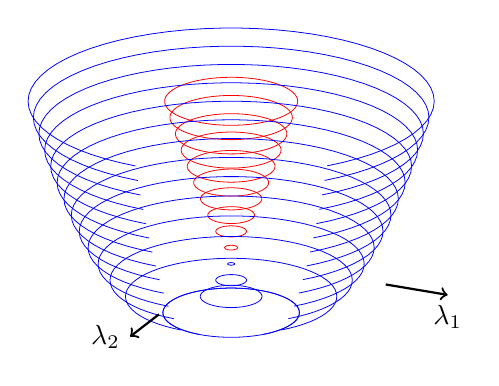
\begin{tikzpicture}
            \begin{axis}[samples=60,hide axis]
                \foreach \zz in {0.2,0.5,...,3}
                {
                   \addplot3[domain=0:6.28, line width=0.1mm, mark=none, color=red, samples y=0]
                   ({(sqrt(\zz+1)-1) * cos(deg(x))}, {(sqrt(\zz+1)-1) * sin(deg(x))}, {\zz});
                }
                \foreach \zz in {-1,-0.7,...,0}
                {
                   \addplot3[domain=0:6.28, line width=0.1mm, mark=none, color=blue, samples y=0]
                   ({(sqrt(\zz+1)-1) * cos(deg(x))}, {(sqrt(\zz+1)-1) * sin(deg(x))}, {\zz});
                }
                \foreach \zz in {-1,-0.7,...,3}{
                   \addplot3[domain=2.5:7.8, line width=0.1mm, mark=none, color=blue, samples y=0]
                   ({(-sqrt(\zz+1)-1) * cos(deg(x))}, {(-sqrt(\zz+1)-1) * sin(deg(x))}, {\zz});
                }
                \draw[->,thick] (2.5,0,0)--(3.5,0,0)node[below]{\(\lambda_1\)};
                \draw[->,thick] (0,-2.5,0)--(0,-3.5,0)node[left]{\(\lambda_2\)};
            \end{axis}
        \end{tikzpicture}
        \caption{The energy of the two \(^2E_g\) electronic states of a \(\mathrm{d}^9\) complex against two vibration coordinates of \(E_g\) symmetry. The scale of the distortion along the two modes are \(\lambda_1\) and \(\lambda_2\) respectively, and the energy of one of the electronic states (the blue one) has its minima at non-zero magnitude of distortions, leading to the spontaneous symmetry breaking of the complex.}
    \end{figure}

    Therefore, the \(\mathrm{d}^9\) complexes will be distorted and the double degeneracy of the two \(^2E_g\) electronic states will be broken to allow the molecule to sit in a lower energy non-degenerate electronic state. 

    \subsubsection{Jahn--Teller Distortion in Octahedral \texorpdfstring{\(\mathrm{d}^8\)}{d8} Complexes}
    The situation for the \(\mathrm{d}^8\) complexes is more subtle. The electron configuration is \(e_g^2\) and the allowed terms are \(^1E_g\), \(^1A_{1g}\) and \(^3 A_{2g}\). By Hund's first rule, the lowest energy state in the octahedral geometry is \(^3A_{2g}\), with \(^1E_g\) above it and the \(^1A_{1g}\) above that. However, \(^1E_g\) is degenerate, so it is subjected to Jahn--Teller distortion of \(E_g\) symmetry, which may reduce the energy below that of triplet. Consequently in \(\mathrm{d}^8\) we may get either a symmetric triplet state or a distorted singlet state.

    \begin{figure}
        \centering
        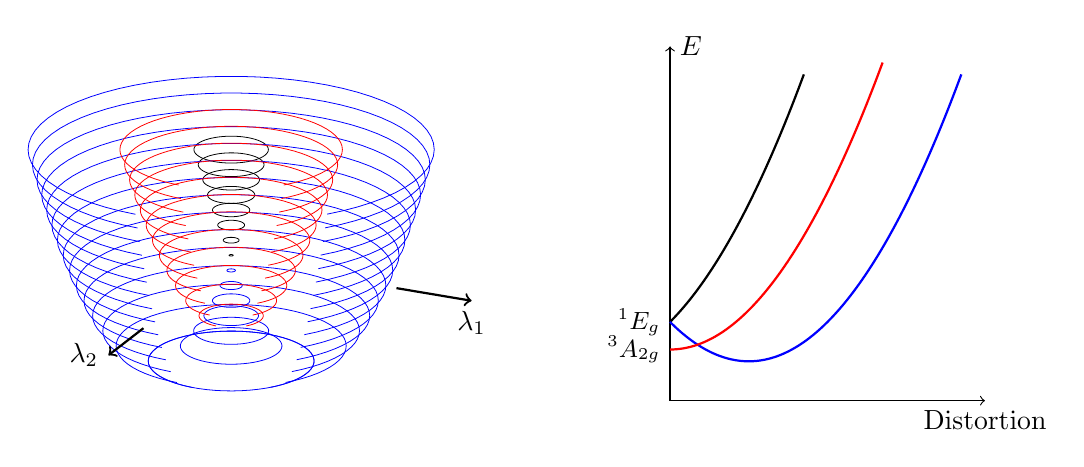
\begin{tikzpicture}
            \begin{axis}[samples=60,hide axis]
                \foreach \zz in {0.05,0.20,...,1.1}
                {
                   \addplot3[domain=0:6.28, line width=0.1mm, mark=none, color=black, samples y=0]
                   ({(sqrt(\zz+1)-1) * cos(deg(x))}, {(sqrt(\zz+1)-1) * sin(deg(x))}, {\zz});
                }
                \foreach \zz in {-1,-0.85,...,0}
                {
                   \addplot3[domain=0:6.28, line width=0.1mm, mark=none, color=blue, samples y=0]
                   ({(sqrt(\zz+1)-1) * cos(deg(x))}, {(sqrt(\zz+1)-1) * sin(deg(x))}, {\zz});
                }
                \foreach \zz in {-1,-0.85,...,1.1}{
                   \addplot3[domain=2.5:7.8, line width=0.1mm, mark=none, color=blue, samples y=0]
                   ({(-sqrt(\zz+1)-1) * cos(deg(x))}, {(-sqrt(\zz+1)-1) * sin(deg(x))}, {\zz});
                }
                \foreach \zz in {-0.7,-0.55,...,1.1}{
                   \addplot3[domain=-0.642:4.658, line width=0.1mm, mark=none, color=red, samples y=0]
                   ({sqrt(\zz+0.7) * cos(deg(x))}, {sqrt(\zz+0.7) * sin(deg(x))}, {\zz});
                }
                \draw[->,thick] (2.2,0,0)--(3.2,0,0)node[below]{\(\lambda_1\)};
                \draw[->,thick] (0,-2.5,0)--(0,-3.5,0)node[left]{\(\lambda_2\)};
            \end{axis}
            \begin{scope}[shift={(9,1)}]
                \draw[->] (0,0)--(4,0)node[below]{Distortion};
                \draw[->] (0,0)--(0,4.5)node[right]{\(E\)};
                \draw[thick,domain=0:1.7, smooth, variable=\x,samples=50] plot ({\x}, {1+0.5*\x*\x+\x});
                \draw[thick,domain=0:3.7, smooth, variable=\x,samples=50,blue] plot ({\x}, {1+0.5*\x*\x-\x});
                \draw[thick,domain=0:2.7, smooth, variable=\x,samples=50,red] plot ({\x}, {0.65+0.5*\x*\x});
                \node at (0,1)[left]{\small\(\quad ^1E_g\)};
                \node at (0,0.65)[left]{\small\(^3A_{2g}\)};
            \end{scope}
        \end{tikzpicture}
        \caption{The energy of the electronic states of a \(\mathrm{d}^8\) complex against distortion. In the undistorted octahedral complex, the \(^3A_{2g}\) is the ground state, but the \(^1E_g\) state is subjected to Jahn--Teller distortion, which may or may not reduce its energy below the triplet state.}
    \end{figure}

    \subsubsection{The Dynamical Jahn--Teller Effect}
    In some molecules the energy associated with the Jahn--Teller distortion is small compared with \(k_B T\), and then the distortion is not static but dynamic. This does not occur in the octahedral \(\mathrm{d}^9\) complexes, where there is a strong interaction between the \(e_g\) orbitals and the ligands, but it is common in complexes where only the \(t_{2g}\) orbitals are occupied, since these interact much more weakly with the ligands.

    \newpage
    \section{Vibrational Coordinates}
    Now let's turn to investigate the vibrations in a molecular system. In a molecule of \(N\) atoms, each atom has \(3\) Cartesian displacement coordinates, so they form a basis of a \(3N\)-dimensional representation. We can reduce this representation in just the same way we did for molecular orbitals, and we will get \(3N\) symmetry-adapted vibration coordinates. Three of these will correspond to the translation of the whole molecule, and another three of these correspond to rotations (or two for linear molecules). Subtracting these off, we are left with \(3N-6\) (or \(3N-5\)) vibrational normal modes. This should be familiar from IB Chemistry A and A3: \textit{High Resolution Molecular Spectroscopy}.

    \begin{ex}
        For \(\mathrm{BF_3}\) molecule with point group \(D_{3h}\), the \(3N\) Cartesian displacement vectors transform as \(A_1'\oplus A_2'\oplus 2A_2''\oplus 3E'\oplus E''\). The translations transform as \(A_2''\oplus E'\), and the rotations transform as \(A_2'\oplus E''\), leaving the vibrations \(A_1'\oplus A_2''\oplus 2E'\).

        \begin{figure}[ht!]
            \centering
            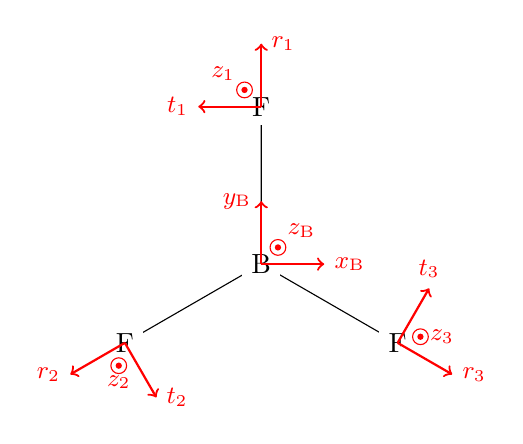
\begin{tikzpicture}
                \coordinate (B) at (0,0);
                \coordinate (F1) at (90:2);
                \coordinate (F2) at (210:2);
                \coordinate (F3) at (330:2);
                \draw (F1)node[fill=white]{F}--(B)--(F2)node[fill=white]{F};
                \draw (F3)node[fill=white]{F}--(B)node[fill=white]{B};
                \draw[red,thick,->] (B)--+(0:0.8)node[right]{\small\(x_{\mathrm{B}}\)};
                \draw[red,thick,->] (B)--+(90:0.8)node[left]{\small\(y_{\mathrm{B}}\)};
                \fill[red] ($(B) + (45:0.3)$) circle (0.04);
                \draw[red] ($(B) + (45:0.3)$)node[above right]{\small\(z_{\mathrm{B}}\)} circle (0.1);
                \draw[red,thick,->] (F1)--+(90:0.8)node[right]{\small\(r_1\)};
                \draw[red,thick,->] (F1)--+(180:0.8)node[left]{\small\(t_1\)};
                \fill[red] ($(F1) + (135:0.3)$) circle (0.04);
                \draw[red] ($(F1) + (135:0.3)$)node[above left]{\small\(z_1\)} circle (0.1);
                \draw[red,thick,->] (F2)--+(210:0.8)node[left]{\small\(r_2\)};
                \draw[red,thick,->] (F2)--+(300:0.8)node[right]{\small\(t_2\)};
                \fill[red] ($(F2) + (255:0.3)$) circle (0.04);
                \draw[red] ($(F2) + (255:0.3)$)node[below]{\small\(z_2\)} circle (0.1);
                \draw[red,thick,->] (F3)--+(-30:0.8)node[right]{\small\(r_3\)};
                \draw[red,thick,->] (F3)--+(60:0.8)node[above]{\small\(t_3\)};
                \fill[red] ($(F3) + (15:0.3)$) circle (0.04);
                \draw[red] ($(F3) + (15:0.3)$)node[right]{\small\(z_3\)} circle (0.1);
            \end{tikzpicture}
        \end{figure}

        It is non-trivial to work out the vibration coordinates --- some are easier to guess, while others are not. You will explore how to compute this in \textit{C7: Further Quantum Mechanics} or in Part IB Mathematics. Here we will state some of the results. The totally symmetric \(A_1'\) mode is the symmetric combination of the fluorine radial displacements
        \begin{equation}
            Q_{A_1'}=\sqrt{\frac{1}{3}}(r_1+r_2+r_3)\,.
        \end{equation}
        The \(A_2''\) mode is a linear combination of \(z_{\mathrm{B}}\) and the symmetric combination of the fluorine \(z\) displacements
        \begin{equation}
            Q_{A_2''}=c_1 z_{\mathrm{B}}+c_2\left(z_1+z_2+z_3\right)\,,
        \end{equation}
        where coefficients \(c_1\) and \(c_2\) are chosen to leave the centre of mass stationary. The doubly degenerate \(E'\) modes are slightly more complicated. The first pair are formed by the radial movements of the F atoms, balanced by the opposite movement of B
        \begin{align}
            Q_{1E'_x}&=d_1 x_{\mathrm{B}}+d_2(r_3-r_2)\,, \\
            Q_{1E'_y}&=d_3 y_{\mathrm{B}}+d_4(2r_1-r_2-r_3)\,,
        \end{align}
        and the second pair are from the tangential movements of the F atoms
        \begin{align}
            Q_{2E'_x}&=e_1 x_{\mathrm{B}}+e_2(2t_1-t_2-t_3)\,, \\
            Q_{2E'_y}&=e_3 y_{\mathrm{B}}+e_4(t_3-t_2)\,.
        \end{align}
        The constants \(d_i,e_i\) are again to make the centre of the molecule stationary.
    \end{ex}

    \subsection{Allowed Harmonic Terms in Vibrational Potential}
    Normally the potential energy for the nuclear motion is some complex function of the nuclear coordinates that we will expand in a Taylor series about the equilibrium geometry. This makes all the linear terms vanish, so the leading order terms we need to consider are the quadratic terms. Under this approximation, the vibrational potential is harmonic.

    However, the Hamiltonian should be totally symmetric, so only the symmetric terms can appear. If we have a set of vibrational coordinates \((Q_{a1},Q_{a2},\dots)\) transforming as the irreducible representation \(\Gamma^a\), and another set \((Q_{b1},Q_{b2},\dots)\) transforming as \(\Gamma^b\), then the possible quadratic terms \(Q_{ai}Q_{bj}\) transform as the direct product \(\Gamma^a\otimes\Gamma^b\). Since all vibrational coordinates we are going to consider are real, this set of elements includes a single symmetric component if and only if \(\Gamma^a\sim\Gamma^b\), and if \(\Gamma^a=\Gamma^b\), the symmetric component is proportional to \(\sum_i Q_{ai}Q_{bi}\).

    \begin{ex}
        The only quadratic terms that may appear in the vibrational potential of \(\mathrm{BF_3}\) are
        \begin{equation}
            Q_{A_1'}^2\,,\ Q_{A_2''}^2\,,\ Q_{1E'_x}^2+Q_{1E'_y}^2\,,\ Q_{2E'_x}^2+Q_{2E'_y}^2\text{ and }Q_{1E'_x}Q_{2E'_x}+Q_{1E'_y}Q_{2E'_y}\,.
        \end{equation}
    \end{ex}

    If we introduce anharmonicity, i.e. consider cubic terms and above, there will be a lot more possibilities.\footnote{The contents beyond this point are non-examinable.}

    \begin{ex}
        Consider again \(\mathrm{BF_3}\). We would like to find the cubic terms that transform totally symmetrically. The possibilities are
        \begin{enumerate}[topsep=0pt,label=(\roman*)]
            \item Any of the harmonic terms can be multiplied by \(Q_{A_1'}\), since \(A_1'\otimes A_1'=A_1'\).
            \item If we can construct a quadratic term transforming as \(A_2''\), then we can multiply it by \(Q_{A_2''}\) to get an \(A_1'\) cubic term. However, the only quadratic \(A_2''\) term is \(Q_{A_1'}Q_{A_2''}\), giving a cubic term \(Q_{A_1'}Q_{A_2''}^2\). This situation is included in (i).
            \item We can construct a quadratic \(E'\) term from any two \(E'\otimes E'\). The product of this quadratic \(E'\) with another \(E'\) will give a cubic \(A_1'\) component. For example, a quadratic \(E'\) term can be constructed from the product of \((Q_{1E'_x},Q_{1E'_y})\) with itself, and we obtain \((Q_{1E'_x}^2-Q_{1E'_y}^2,-2Q_{1E'_x}Q_{1E'_y})\). We defined it in a way such that it forms the identical (not just equivalent) \(E'\) representations like the others (i.e. like \((x,y)\)). The \(A_1'\) component of the direct product of it with \((Q_{1E'_x},Q_{1E'_y})\) is then
            \begin{equation}
                Q_{1E'_x}(Q_{1E'_x}^2-Q_{1E'_y}^2)+Q_{1E'_y}(-2Q_{1E'_x}Q_{1E'_y})=Q_{1E'_x}^3-3Q_{1E'_x}Q_{1E'_y}^2\,.
            \end{equation}
            Other terms of this form can be constructed using the \(Q_{2E'}\) components in the triple direct product.
        \end{enumerate}

        No other cubic terms may appear in the Hamiltonian.
    \end{ex}

    Anharmonicity can lead to coupling between vibrational states, and hence to perturbations of their energies. Because the Hamiltonian is symmetric, they can only couple states of the same symmetry. See Fermi resonance later.

    \subsection{Ladder Operators}
    The Hamiltonian of a general harmonic oscillator is
    \begin{equation}
        \hat{H}=-\frac{\hbar^2}{2m}\pdv[2]{}{Q}+\frac{1}{2}kQ^2\,.
    \end{equation}
    As you have seen in IB Chemistry A: \textit{Introduction to Quantum Mechanics}, if we define the length scale \(s=(\hbar^2/mk)^{1/4}\) and the scaled coordinate \(x=Q/s\), and we express the energy in \(\hbar\sqrt{k/m}=\hbar\omega\), then this Hamiltonian reduces to
    \begin{equation}
        \hat{H}=-\frac{1}{2}\pdv[2]{}{x}+\frac{1}{2}x^2\,.
    \end{equation}
    We call this the standard harmonic oscillator --- every harmonic oscillator is the same up to some scaling.

    Next, we make some seemingly arbitrary definition of the \textit{ladder operator}
    \begin{equation}
        \hat{A}\coloneqq\sqrt{\frac{1}{2}}\left(x+\pdv{}{x}\right)
    \end{equation}
    and its Hermitian conjugate
    \begin{equation}
        \hat{A}^\dagger=\sqrt{\frac{1}{2}}\left(x-\pdv{}{x}\right)\,.
    \end{equation}
    The motivation of doing so is that it somehow ``factorises'' the Hamiltonian such that for any \(\psi\),
    \begin{equation}
        \hat{A}\hat{A}^\dagger\psi=\frac{1}{2}\left(x+\pdv{}{x}\right)\left(x-\pdv{}{x}\right)\psi=\frac{1}{2}\left(x^2-\pdv[2]{}{x}+1\right)=\left(\hat{H}+\frac{1}{2}\right)\psi\,,
    \end{equation}
    and so
    \begin{equation}
        \hat{A}\hat{A}^\dagger=\hat{H}+\frac{1}{2}\,.
    \end{equation}
    Similarly one can show that
    \begin{equation}
        \hat{A}^\dagger\hat{A}=\hat{H}-\frac{1}{2}\,.
    \end{equation}

    Now suppose there is a wavefunction \(\psi_n\) that is an eigenfunction of \(\hat{H}\) such that
    \begin{equation}
        \hat{H}\psi_n=E_n\psi_n\,,
    \end{equation}
    consider the function \(\hat{A}^\dagger\psi_n\), we find
    \begin{align}
        \hat{H}(\hat{A}^\dagger\psi_n) &=(\hat{A}^\dagger\hat{A}+\frac{1}{2})\hat{A}^\dagger\psi_n\notag\\
        &=\hat{A}^\dagger\left(\hat{A}\hat{A}^\dagger+\frac{1}{2}\right)\psi_n\notag\\
        &=\hat{A}^\dagger(\hat{H}+1)\psi_n\notag\\
        &=(E_n+1)(\hat{A}^\dagger\psi_n)\,.
    \end{align}
    This means that if we have an eigenstate \(\psi_n\) with eigenvalue \(E_n\), we can always construct another eigenstate with eigenvalue \(E_n+1\) by acting \(\hat{A}^\dagger\) to it. In the same way, one can show that \(\hat{A}\psi_n\) is also an eigenfunction with energy \(E_n-1\). \(\hat{A}^\dagger\) and \(\hat{A}\) are therefore also called the \textit{raising} and \textit{lowering operators}, respectively.

    Suppose we start from a particular eigenstate of \(\hat{H}\), with eigenvalue \(k\), then it seems that by repeatedly acting \(\hat{A}\) and \(\hat{A}^\dagger\), we can generate a whole sequence of eigenstates with eigenvalues \(k+n\) with \(n\in\mathbb{Z}\), corresponding to energies \((k+n)\hbar\omega\) from negative to plus infinity. However, the energy of a harmonic oscillator cannot be negative,\footnote{We can have a formal justification for this. Consider
    \begin{equation}
        \expval{\hat{H}-\frac{1}{2}}{\psi_n}=\expval{\hat{A}^\dagger\hat{A}}{\psi_n}=\norm{\hat{A}\ket{\psi_n}}^2\ge 0
    \end{equation}
    since the norm is always non-negative. Hence \(\expval{\hat{H}}{\psi_n}=E_n\ge \frac{1}{2}\).} so we cannot infinitely act \(\hat{A}\) on an eigenstate --- the lowering process must terminate at some point and we must have a particular eigenstate \(\psi_0\) with \(\hat{A}\psi_0=0\), after which keep acting \(\hat{A}\) gives nothing. We can solve for this state:\footnote{This is a first order linear homogeneous ODE --- much easier than the original second order eigenvalue problem. Everyone should be able to solve it.}
    \begin{equation}
        \hat{A}\psi_0=\sqrt{\frac{1}{2}}\left(x+\pdv{}{x}\right)\psi_0=0\,,
    \end{equation}
    giving the (unnormalised) wavefunction
    \begin{equation}
        \psi_0=\exp\left(-\frac{1}{2}x^2\right)\,.
    \end{equation}
    This is the state of the lowest energy, also known as the ground state, with eigenvalue
    \begin{equation}
        \hat{H}\psi_0=\left(\hat{A}^\dagger\hat{A}+\frac{1}{2}\right)\psi_0=\frac{1}{2}\psi_0
    \end{equation}
    in units of \(\hbar\omega\). The wavefunctions of the other vibrational excited states are
    \begin{equation}
        \psi_n=(\hat{A}^\dagger)^n\psi_0
    \end{equation}
    with energies \((n+\frac{1}{2})\hbar\omega\).

    \subsubsection{Symmetries of the Vibrational States}
    Let's consider the symmetry of the vibrational eigenstates. First consider the non-degenerate case where the scaled vibrational coordinate \(x=Q/s\) scales as some one-dimensional representation \(\Gamma^Q\). Then since \(x^2\) will always transform as \(\Gamma^Q\otimes\Gamma^Q=\Gamma^{(1)}\), the wavefunction
    \begin{equation}
        \psi_0=\exp\left(-\frac{1}{2}x^2\right)
    \end{equation}
    is also totally symmetric. Since \(\hat{A}^\dagger\) has the same symmetry as \(x\) (obvious from its definition),
    \begin{equation}
        \psi_1=\hat{A}^\dagger\psi_0
    \end{equation}
    must transform as \(\Gamma^{Q}\otimes\Gamma^{(1)}=\Gamma^{Q}\), the same irreducible representation as the vibrational coordinate \(Q\). Next,
    \begin{equation}
        \psi_2=\hat{A}^\dagger\psi_1
    \end{equation}
    will transform as \(\Gamma^{Q}\otimes\Gamma^{Q}=\Gamma^{(1)}\), so it is again totally symmetric. We can see that this alternating pattern carries on. For non-degenerate vibrations, the vibrational states \(\psi_n\) alternate between totally symmetric (for even \(n\)) and the same symmetry as the vibrational coordinate (odd \(n\)).

    For degenerate vibration with coordinates \((x_1,x_2,\dots)\) transforming as an irreducible representation \(\Gamma^Q\) with dimension larger than one, there is a pair of ladder operators \(\hat{A}\) and \(\hat{A}^\dagger\) for each \(x_i\). The ground state has zero quanta of excitation in each mode, and it is
    \begin{equation}
        \psi_{00\dots}=\exp\left(-\frac{1}{2}(x_1^2+x_2^2+\dots)\right)\,.
    \end{equation}
    This is again totally symmetric. There is a set of singly-excited states
    \begin{equation}
        \hat{A}_i^\dagger\psi_{00\dots}\,,
    \end{equation}
    which together transform like the \(\hat{A}_i^\dagger\) and hence like \((x_1,x_2,\dots)\), with irreducible representation \(\Gamma^Q\). The doubly-excited states are
    \begin{equation}
        \hat{A}_i^\dagger\hat{A}_j^\dagger\psi_{00\dots}\,,
    \end{equation}
    transforming as the products \(\hat{A}_i^\dagger\hat{A}_j^\dagger\). But since \(\hat{A}_i^\dagger\hat{A}_j^\dagger=\hat{A}_j^\dagger\hat{A}_i^\dagger\), we only get the components of the symmetrised square.

    \subsection{Fermi Resonance}
    As we claimed above, due to anharmonicity, there may be coupling between vibrational states of the same symmetry. This is best illustrated with an example.
    \begin{ex}
        The vibrational modes of \(\mathrm{CO_2}\) with \(D_{\infty h}\) point group have irreducible representations \(\Sigma_g^+\oplus\Pi_u\oplus\Sigma_u^+\) (we will label the vibrational states in this order). The bending vibration \(v_2\) has symmetry \(\Pi_u\) and frequency \(\tilde{\nu}_2=667\unit{cm}^{-1}\). We will label the first excited state of this mode by \(01^10\), where the superscript for a degenerate mode indicates that this mode has an angular momentum \(\pm 1\) about the molecular axis (and hence it has symmetry \(\Pi\)). The doubly-excited state of this mode has symmetry \((\Pi_u\otimes\Pi_u)_+=\Sigma_g^+\oplus\Delta_g\), and are denoted \(02^00\) and \(02^20\) respectively. They will have energy \(2\tilde{\nu}_2=1334\unit{cm}^{-1}\)

        \begin{figure}[ht!]
            \centering
            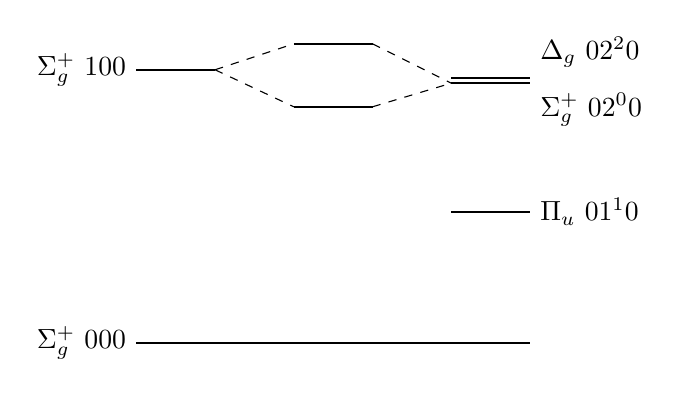
\begin{tikzpicture}
                \draw[thick] (0,0)node[left]{\(\Sigma_g^+\ 000\)}--(5,0);
                \draw[thick] (0,3.47)node[left]{\(\Sigma_g^+\ 100\)}--(1,3.47);
                \draw[thick] (4,1.668)--(5,1.668)node[right]{\(\Pi_u\ 01^10\)};
                \draw[thick] (4,3.30)--(5,3.30)node[below right]{\(\Sigma_g^+\ 02^00\)};
                \draw[thick] (4,3.37)--(5,3.37)node[above right]{\(\Delta_g\ 02^20\)};
                \draw[thick] (2,3)--(3,3);
                \draw[thick] (2,3.8)--(3,3.8);
                \draw[dashed] (1,3.47)--(2,3);
                \draw[dashed] (1,3.47)--(2,3.8);
                \draw[dashed] (3,3.0)--(4,3.30);
                \draw[dashed] (3,3.8)--(4,3.30);
            \end{tikzpicture}
            \caption{Fermi Resonances in \(\mathrm{CO_2}\).}
        \end{figure}

        However, we find that the symmetric stretch \(v_1\) mode also has \(\Sigma^+\) symmetry with frequency \(\tilde{\nu}_1=1388\unit{cm}^{-1}\), meaning that the first excited state of this mode, denoted \(100\), has symmetry \(\Sigma^+\) and energy \(\tilde{\nu}_1=1388\unit{cm}^{-1}\) above the ground state. We have two states \(100\) and \(02^00\) with the same symmetry and close in energy, so they will interact, just like two orbitals with the same symmetry and similar energy will interact. This is possible since there will be an anharmonic term in the Hamiltonian proportional to \(Q_1(Q_{2x}^2+Q_{2y}^2)=Q_1Q_{2\text{sym}}^2\). The two states are therefore mixed, resulting in a splitting in energy. The strength of the coupling is
        \begin{equation}
            \mel{02^00}{V_{\text{anh}}}{100}=\frac{1}{2}\left(\frac{\partial^3 V}{{\partial Q_{2\text{sym}}}^2\partial Q_1}\right)\mel{0}{Q_1}{1}\mel{2^0}{Q_{2\text{sym}}^2}{0}\braket{0}{0}\,,
        \end{equation}
        where there are three equivalent contributions so the factor of \(\frac{1}{3!}\) in the Taylor expansion of the potential becomes \(\frac{1}{2}\).
    \end{ex}
    \newpage
    \section{More on Symmetry Operations}
    \subsection{Non-Rigid Molecules}
    Let's consider the ammonia molecule. There are six possible permutations of the three protons, which can be labelled \(E\), \((ab)\), \((ac)\), \((bc)\), \((abc)\) and \((acb)\). All of them can be combined with the inversion \(E^*\) operation to give another six permutation-inversions. These are twelve operations altogether, but the symmetry group of \(\mathrm{NH_3}\) is \(C_{3v}\), which contains only six elements. Which six of the twelve do these correspond to, and what do the other six operations do?

    Using the same method as what we did for \(\mathrm{H_2O}\) in chapter 1, we find that \((abc)\) and \((acb)\) correspond to \(C_3\) and \(C_3^{-1}\), and \((ab)^*\), \((bc)^*\) and \((ac)^*\) correspond to the three reflections in \(C_{3v}\) group. What does other permutation-inversion operations do? Let's use \(E^*\) as an example. We define the \(z\) axis to be along the principal axis and at the opposite side of the \(\mathrm{H}\) atoms, \(x\) axis so that \(xz\) plane contains atom \(a\), and \(y\) to complete the right-handed frame. You will find that it is impossible to reorient the molecule transformed by \(E^*\) to align it with the original molecule. For example, if you choose to make the atoms \(\mathrm{N}\) and \(\mathrm{H}_a\) coincide with the original molecule, then the \(b\) and \(c\) are necessarily in the wrong order.

    \begin{figure}[ht!]
        \centering
        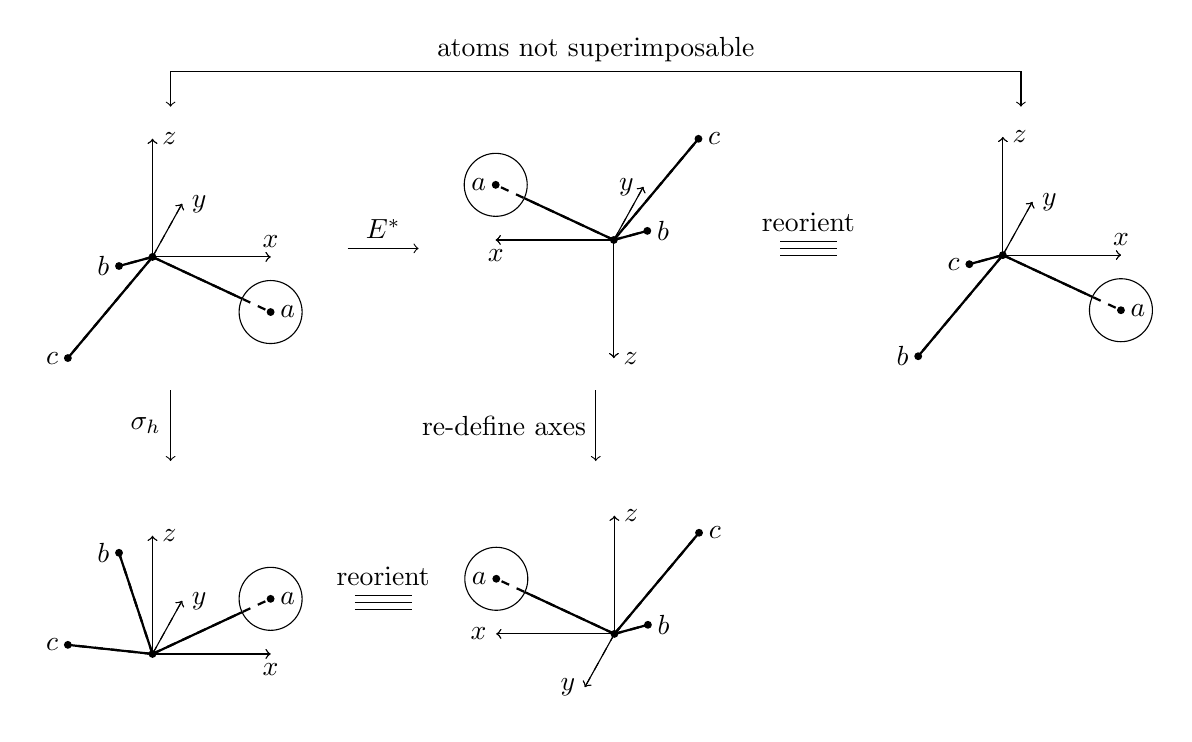
\begin{tikzpicture}[scale=0.9]
            \node at (0,0){\tikz[z={(-0.25cm,-0.45cm)}]{
                \coordinate (a) at (1.5,-0.7,0);
                \coordinate (b) at (-0.75,-0.7,-1.299);
                \coordinate (c) at (-0.75,-0.7,1.299);
                \draw[thick] (0,0,0)--(a);
                \draw[thick] (0,0,0)--(b);
                \draw[thick] (0,0,0)--(c);
                \draw[->] (0,0,0)--(1.5,0,0);
                \draw[->] (0,0,0)--(0,1.5,0);
                \draw[->] (0,0,0)--(0,0,-1.5);
                \draw[fill=white] (a) circle (0.4);
                \draw[thick,dashed] (0,0,0)--(a);
                \draw[thick,dashed] (0,0,0)--(b);
                \draw[thick,dashed] (0,0,0)--(c);
                \draw[->,dashed] (0,0,0)--(1.5,0,0)node[above]{\(x\)};
                \draw[->,dashed] (0,0,0)--(0,1.5,0)node[right]{\(z\)};
                \draw[->,dashed] (0,0,0)--(0,0,-1.5)node[right]{\(y\)};
                \fill[black] (0,0,0) circle (0.05);
                \fill[black] (a)node[right]{\(a\)} circle (0.05);
                \fill[black] (b)node[left]{\(b\)} circle (0.05);
                \fill[black] (c)node[left]{\(c\)} circle (0.05);
            }};

            \draw[->] (2.5,0)--node[above]{\(E^*\)}(3.5,0);

            \node at (6,0){\tikz[z={(-0.25cm,-0.45cm)}]{
                \coordinate (a) at (-1.5,0.7,0);
                \coordinate (b) at (0.75,0.7,1.299);
                \coordinate (c) at (0.75,0.7,-1.299);
                \draw[thick] (0,0,0)--(a);
                \draw[thick] (0,0,0)--(b);
                \draw[thick] (0,0,0)--(c);
                \draw[->] (0,0,0)--(-1.5,0,0);
                \draw[->] (0,0,0)--(0,-1.5,0);
                \draw[->] (0,0,0)--(0,0,-1.5);
                \draw[fill=white] (a) circle (0.4);
                \draw[thick,dashed] (0,0,0)--(a);
                \draw[thick,dashed] (0,0,0)--(b);
                \draw[thick,dashed] (0,0,0)--(c);
                \draw[->,dashed] (0,0,0)--(-1.5,0,0)node[below]{\(x\)};
                \draw[->,dashed] (0,0,0)--(0,-1.5,0)node[right]{\(z\)};
                \draw[->,dashed] (0,0,0)--(0,0,-1.5)node[left]{\(y\)};
                \fill[black] (0,0,0) circle (0.05);
                \fill[black] (a)node[left]{\(a\)} circle (0.05);
                \fill[black] (b)node[right]{\(b\)} circle (0.05);
                \fill[black] (c)node[right]{\(c\)} circle (0.05);
            }};

            \foreach \i in {-1,0,1}{
                \draw (8.6,0.1*\i)--(9.4,0.1*\i);
            }
            \node at (9,0.1)[above]{reorient};

            \node at (12,0){\tikz[z={(-0.25cm,-0.45cm)}]{
                \coordinate (a) at (1.5,-0.7,0);
                \coordinate (c) at (-0.75,-0.7,-1.299);
                \coordinate (b) at (-0.75,-0.7,1.299);
                \draw[thick] (0,0,0)--(a);
                \draw[thick] (0,0,0)--(b);
                \draw[thick] (0,0,0)--(c);
                \draw[->] (0,0,0)--(1.5,0,0);
                \draw[->] (0,0,0)--(0,1.5,0);
                \draw[->] (0,0,0)--(0,0,-1.5);
                \draw[fill=white] (a) circle (0.4);
                \draw[thick,dashed] (0,0,0)--(a);
                \draw[thick,dashed] (0,0,0)--(b);
                \draw[thick,dashed] (0,0,0)--(c);
                \draw[->,dashed] (0,0,0)--(1.5,0,0)node[above]{\(x\)};
                \draw[->,dashed] (0,0,0)--(0,1.5,0)node[right]{\(z\)};
                \draw[->,dashed] (0,0,0)--(0,0,-1.5)node[right]{\(y\)};
                \fill[black] (0,0,0) circle (0.05);
                \fill[black] (a)node[right]{\(a\)} circle (0.05);
                \fill[black] (b)node[left]{\(b\)} circle (0.05);
                \fill[black] (c)node[left]{\(c\)} circle (0.05);
            }};
            \draw[<->] (0,2)--(0,2.5)--node[above]{atoms not superimposable}(12,2.5)--(12,2);


            \draw[->] (0,-2)--node[left]{\(\sigma_h\)}(0,-3);

            \node at (0,-5){\tikz[z={(-0.25cm,-0.45cm)}]{
                \coordinate (a) at (1.5,0.7,0);
                \coordinate (b) at (-0.75,0.7,-1.299);
                \coordinate (c) at (-0.75,0.7,1.299);
                \draw[thick] (0,0,0)--(a);
                \draw[thick] (0,0,0)--(b);
                \draw[thick] (0,0,0)--(c);
                \draw[->] (0,0,0)--(1.5,0,0);
                \draw[->] (0,0,0)--(0,1.5,0);
                \draw[->] (0,0,0)--(0,0,-1.5);
                \draw[fill=white] (a) circle (0.4);
                \draw[thick,dashed] (0,0,0)--(a);
                \draw[thick,dashed] (0,0,0)--(b);
                \draw[thick,dashed] (0,0,0)--(c);
                \draw[->,dashed] (0,0,0)--(1.5,0,0)node[below]{\(x\)};
                \draw[->,dashed] (0,0,0)--(0,1.5,0)node[right]{\(z\)};
                \draw[->,dashed] (0,0,0)--(0,0,-1.5)node[right]{\(y\)};
                \fill[black] (0,0,0) circle (0.05);
                \fill[black] (a)node[right]{\(a\)} circle (0.05);
                \fill[black] (b)node[left]{\(b\)} circle (0.05);
                \fill[black] (c)node[left]{\(c\)} circle (0.05);
            }};

            \draw[->] (6,-2)--node[left]{re-define axes}(6,-3);

            \node at (6,-5){\tikz[z={(-0.25cm,-0.45cm)}]{
                \coordinate (a) at (-1.5,0.7,0);
                \coordinate (b) at (0.75,0.7,1.299);
                \coordinate (c) at (0.75,0.7,-1.299);
                \draw[thick] (0,0,0)--(a);
                \draw[thick] (0,0,0)--(b);
                \draw[thick] (0,0,0)--(c);
                \draw[->] (0,0,0)--(-1.5,0,0);
                \draw[->] (0,0,0)--(0,1.5,0);
                \draw[->] (0,0,0)--(0,0,1.5);
                \draw[fill=white] (a) circle (0.4);
                \draw[thick,dashed] (0,0,0)--(a);
                \draw[thick,dashed] (0,0,0)--(b);
                \draw[thick,dashed] (0,0,0)--(c);
                \draw[->,dashed] (0,0,0)--(-1.5,0,0)node[left]{\(x\)};
                \draw[->,dashed] (0,0,0)--(0,1.5,0)node[right]{\(z\)};
                \draw[->,dashed] (0,0,0)--(0,0,1.5)node[left]{\(y\)};
                \fill[black] (0,0,0) circle (0.05);
                \fill[black] (a)node[left]{\(a\)} circle (0.05);
                \fill[black] (b)node[right]{\(b\)} circle (0.05);
                \fill[black] (c)node[right]{\(c\)} circle (0.05);
            }};

            \foreach \i in {-1,0,1}{
                \draw (2.6,-5+0.1*\i)--(3.4,-5+0.1*\i);
            }
            \node at (3,-4.9)[above]{reorient};
           
        \end{tikzpicture}
        \caption{An ammonia molecule transformed by parity inversion \(E^*\) is identical to the flipped ammonia molecule. We can regard it as a \(\sigma_h\) operation which is not in the symmetry group of ammonia.}
    \end{figure}

    The new configuration of ammonia generated by the \(E^*\) operation is not superimposable on the original one --- it is a mirror image. It is a second version of the equilibrium geometry, distinguishable from the first if we take nuclear labels into account. Moreover, it is accessible from the original configuration by ``flipping'' the configuration of the molecule via a planar transition structure, with a low energy barrier of \(25\unit{kJ}\unit{mol}^{-1}\).

    The vibrational wavefunction of the two versions of ammonia can also mix by tunnelling through the barrier, leading to a small but observable splitting of the vibrational energy level. The wavefunctions are either symmetric or antisymmetric with respect to the \(E^*\) operation, so we need it to get a complete symmetry classification.

    \begin{figure}
        \centering
        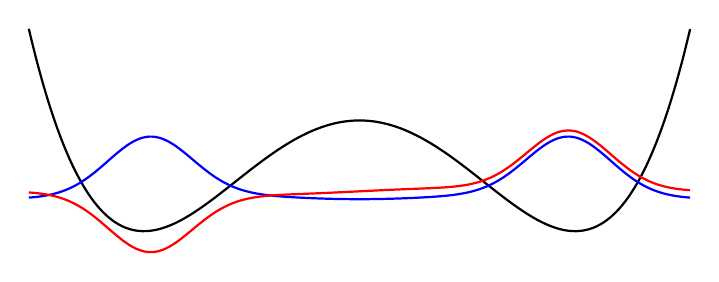
\begin{tikzpicture}
            \draw[thick,domain=-2.1:2.1, smooth, variable=\x,samples=100] plot ({2*\x}, {0.4*\x*\x*\x*\x-1.5*\x*\x});
            \draw[thick,domain=-2.1:2.1, blue, smooth, variable=\x,samples=100] plot ({2*\x}, {0.75*2.72^(-7*(\x-1.33)*(\x-1.33))+0.75*2.72^(-7*(\x+1.33)*(\x+1.33))+0.15*\x*\x*2.72^(-\x*\x)-1});
            \draw[thick,domain=-2.1:2.1, red, smooth, variable=\x,samples=100] plot ({2*\x}, {0.75*2.72^(-7*(\x-1.33)*(\x-1.33))-0.75*2.72^(-7*(\x+1.33)*(\x+1.33))+0.1*\x*2.72^(-\x*\x)-0.9});
        \end{tikzpicture}
        \caption{Vibrational wavefunctions when considering the inversion of ammonia. The wavefunction can be symmetric or antisymmetric with respect to \(E^*\), with a detectable energy gap.}
    \end{figure}

    In ammonia, the two versions of the equilibrium geometry are easily accessible from each other via a low barrier. The operations that convert one version into the other are said to be \textit{feasible}, and we need them for a complete classification of the energy levels.

    Next, let's consider methane molecule, where there are \(24\) permutations of the four \(\mathrm{H}\) atoms, and 24 permutation-inversions. However a half of these lead to an inverted configuration of methane that can only be reached by crossing a very high energy barrier. There is essentially no mixing between the wavefunction of these two versions of methane, and the symmetry operations that convert one into the other do not add any useful information. Such non-feasible operations can be ignored. The \textit{molecular symmetry group} is the set of all feasible permutations and permutation-inversions.

    Ammonia is an example of a \textit{non-rigid molecule}. Such molecules have more than one version of the minimum energy geometry, distinguished from one another by nuclear labels, and connected to each other by low-energy pathways on the potential energy surfaces.

    An important class of such non-rigid molecules comprises weakly-bound \textit{van der Waals} molecules. In the water dimer, for example, one molecule acts as a proton donor to the other to form a hydrogen bond. The resulting structure has a \(C_s\) symmetry. The \(\mathrm{H}\) atom in the hydrogen bond can be any of the four; moreover the two \(\mathrm{H}\) atoms in the acceptor molecule can change places by a feasible motion. Consequently there are eight versions of the equilibrium structure, each having a \(C_s\) symmetry, so there are sixteen symmetry operations in the molecular symmetry group. All of these must be included in order to classify the vibrational states. Often the symmetry groups for the molecules clusters like this do not correspond to any of the standard tabulated symmetry point groups.

    \begin{figure}
        \centering
        \begin{tikzpicture}[x={(0.95cm,-0.1cm)},z={(-0.2cm,-0.4cm)}]
            \begin{scope}
                \draw[thick] (-0.433,0.75,1.224)node[left]{4}--(0,0,0)--(-0.433,0.75,-1.224)node[right]{3};
                \draw[thick] (2,0,0)node[above]{1}--++(0:1.5)--++(-70.5:1.5)node[right]{2};
                \draw[dashed] (0,0,0)--node[above]{\(E\)}(2,0,0);
            \end{scope}
            \begin{scope}[shift={(7cm,0cm)}]
                \draw[thick] (-0.433,0.75,1.224)node[left]{2}--(0,0,0)--(-0.433,0.75,-1.224)node[right]{1};
                \draw[thick] (2,0,0)node[above]{3}--++(0:1.5)--++(-70.5:1.5)node[right]{4};
                \draw[dashed] (0,0,0)--node[above]{\((13)(24)\)}(2,0,0);
            \end{scope}
            \begin{scope}[shift={(0cm,-4cm)}]
                \draw[thick] (-0.433,0.75,1.224)node[left]{3}--(0,0,0)--(-0.433,0.75,-1.224)node[right]{4};
                \draw[thick] (2,0,0)node[above]{1}--++(0:1.5)--++(-70.5:1.5)node[right]{2};
                \draw[dashed] (0,0,0)--node[above]{\((34)\)}(2,0,0);
            \end{scope}
            \begin{scope}[shift={(7cm,-4cm)}]
                \draw[thick] (-0.433,0.75,1.224)node[left]{1}--(0,0,0)--(-0.433,0.75,-1.224)node[right]{2};
                \draw[thick] (2,0,0)node[above]{3}--++(0:1.5)--++(-70.5:1.5)node[right]{4};
                \draw[dashed] (0,0,0)--node[above]{\((1324)\)}(2,0,0);
            \end{scope}
            \begin{scope}[shift={(0cm,-8cm)}]
                \draw[thick] (-0.433,0.75,1.224)node[left]{4}--(0,0,0)--(-0.433,0.75,-1.224)node[right]{3};
                \draw[thick] (2,0,0)node[above]{2}--++(0:1.5)--++(-70.5:1.5)node[right]{1};
                \draw[dashed] (0,0,0)--node[above]{\((12)\)}(2,0,0);
            \end{scope}
            \begin{scope}[shift={(7cm,-8cm)}]
                \draw[thick] (-0.433,0.75,1.224)node[left]{1}--(0,0,0)--(-0.433,0.75,-1.224)node[right]{2};
                \draw[thick] (2,0,0)node[above]{3}--++(0:1.5)--++(-70.5:1.5)node[right]{4};
                \draw[dashed] (0,0,0)--node[above]{\((1423)\)}(2,0,0);
            \end{scope}
            \begin{scope}[shift={(0cm,-12cm)}]
                \draw[thick] (-0.433,0.75,1.224)node[left]{3}--(0,0,0)--(-0.433,0.75,-1.224)node[right]{4};
                \draw[thick] (2,0,0)node[above]{2}--++(0:1.5)--++(-70.5:1.5)node[right]{1};
                \draw[dashed] (0,0,0)--node[above]{\((12)(34)\)}(2,0,0);
            \end{scope}
            \begin{scope}[shift={(7cm,-12cm)}]
                \draw[thick] (-0.433,0.75,1.224)node[left]{1}--(0,0,0)--(-0.433,0.75,-1.224)node[right]{2};
                \draw[thick] (2,0,0)node[above]{4}--++(0:1.5)--++(-70.5:1.5)node[right]{3};
                \draw[dashed] (0,0,0)--node[above]{\((14)(23)\)}(2,0,0);
            \end{scope}
        \end{tikzpicture}
        \caption{Eight possible configurations of water dimers.}
    \end{figure}

    \subsection{Approximate Symmetry and Descent in Symmetry}
    Consider the complex \(\mathrm{[Ni(en)_3]^{2+}}\) (\(\mathrm{en}\)=ethylene diamine), where six nitrogen atoms act as ligands to the metal ion. Formally, the complex has \(D_3\) symmetry only, and the metal \(d\) orbitals transform as \(A_1\oplus 2E\).

    This information does not itself tell us much about the relative energies of the \(d\) orbitals. However the immediate environment of the metal ion is approximately octahedral. In \(O_h\) symmetry we know that the \(d\) orbitals split into \(E_g\oplus T_{2g}\), with \(E_g\) orbitals higher in energy by the crystal-field splitting \(\Delta\), which we can estimate reasonably reliably from our knowledge of true octahedral complexes.

    To determine what happens in \(\mathrm{[Ni(en)_3]^{2+}}\), we use \textit{descent in symmetry}. We start by classifying the orbitals according to the approximate symmetry \(O_h\). Then we investigate the behaviour of the \(O_h\) symmetry orbitals under the symmetry operations that remain in \(D_3\).

    Of the 48 symmetry operations in \(O_h\), only six survive in \(D_3\): the identity, one of the \(C_3\) operations and its inverse, and three of the six dihedral \(C_2\) operations. In the \(O_h\) character table, we delete all columns that do not remain in the \(D_3\), leaving three surviving columns only. For each representation \(\Gamma\) of \(O_h\), these three columns give the character for the surviving elements in \(D_3\). We can reduce this character to determine the corresponding symmetry species in \(D_3\).

    \begin{table}[ht!]
        \centering
        \begin{tabular}{c|ccc|c}
            \hline
            \(O_h\) & \(E\) & \(C_3\) & \(C_2\) & \(D_3\) \\ \hline
            \(A_{1g}\) & \(1\) & \(1\) & \(1\) &  \(A_1\) \\
            \(A_{2g}\) & \(1\) & \(1\) & \(-1\) &  \(A_2\) \\
            \(E_{g}\) & \(2\) & \(-1\) & \(1\) &  \(E\) \\
            \(T_{1g}\) & \(3\) & \(0\) & \(-1\) &  \(A_2\oplus E\) \\
            \(T_{2g}\) & \(3\) & \(0\) & \(1\) &  \(A_1\oplus E\) \\ \hline
        \end{tabular}
        \caption{Descent of symmetry table from \(O_h\) to \(D_3\).}
    \end{table}

    The idea of doing so is that if the molecule has a \(O_h\) symmetry, the \(d\) orbitals split into a doubly degenerate pair \(E_g\) and a triply degenerate pair \(T_{2g}\), with distinct energy. We now make a slight tweak to the system that breaks the symmetry of \(O_h\) into \(D_3\). Since the change is small, we are not expected to see a large change in the energy of the orbitals. But some of the orbitals that were degenerate in the \(O_h\) group will have their degeneracies lifted in the \(D_3\) group as the symmetry is reduced. We then expect a small splitting in the energy levels. In this case, we see that the \(E_g\) orbitals remain degenerate, and are now called \(E\) in \(D_3\), while the degeneracy of the \(T_{2g}\) orbitals is broken, and they are split into an \(A_1\) set and an \(E\) set; symmetry doesn't tell us which of them is higher, but often the application of perturbation theory can answer such questions.

    \begin{figure}
        \centering
        \begin{tikzpicture}
            \draw[thick] (0,0)node[left]{\(T_{2g}\)}--(1,0);
            \draw[thick] (0,3)node[left]{\(E_g\)}--(1,3);
            \draw[thick] (5,-0.1)--(6,-0.1)node[below right]{\(A_1\)};
            \draw[thick] (5,0.1)--(6,0.1)node[above right]{\(E\)};
            \draw[thick] (5,3)--(6,3)node[right]{\(E\)};
            \draw[dashed] (5,-0.1)--(1,0)--(5,0.1);
            \draw[dashed] (1,3)--(5,3);
            \begin{scope}[shift={(0.5cm,5.5cm)}]
                \draw (-1.5,0,0)node[fill=white]{\small\(\mathrm{H_3N}\)}--(1.5,0,0)node[fill=white]{\small\(\mathrm{NH_3}\)};
                \draw (0,1.5,0)node[fill=white]{\small\(\quad\ \mathrm{NH_3}\)}--(0,-1.5,0)node[fill=white]{\small\(\quad\ \mathrm{NH_3}\)};
                \draw (0,0,1.5)--(0,0,-1.5);
                \node at (0,0,2) {\small\(\mathrm{H_3N}\ \ \)};
                \node at (0,0,-2) {\small\(\ \ \mathrm{NH_3}\)};
                \node at (0,0,0)[fill=white]{\small\(\mathrm{Ni}\)};
            \end{scope}

            \begin{scope}[shift={(5.5cm,5.5cm)}]
                \draw [rotate around y=90] (0,1.5) arc (90:0:1.5);
                \draw [rotate around x=90] (0,1.5) arc (90:180:1.5);
                \draw (0,-1.5) arc (-90:0:1.5);
                \draw (-1.5,0,0)node[fill=white]{\small\(\mathrm{N}\)}--(1.5,0,0)node[fill=white]{\small\(\mathrm{N}\)};
                \draw (0,1.5,0)node[fill=white]{\small\(\mathrm{N}\)}--(0,-1.5,0)node[fill=white]{\small\(\mathrm{N}\)};
                \draw (0,0,1.5)node[fill=white]{\small\(\mathrm{N}\)}--(0,0,-1.5)node[fill=white]{\small\(\mathrm{N}\)};
                \node at (0,0,0)[fill=white]{\small\(\mathrm{Ni}\)};
            \end{scope}
        \end{tikzpicture}
        \caption{Thinking of \(\mathrm{[Ni(en)_3]^{2+}}\) as a perturbation to the octahedral species.}
    \end{figure}

    \newpage
    \section{Selection Rules}
    Time-dependent perturbation theory\footnote{See C7: \textit{Further Quantum Mechanics}.} tells us that the transition probability between states \(\ket{\Psi''}\) and \(\ket{\Psi'}\) when an oscillatory perturbation \(V\cos\omega t\) is applied is proportional to \(\abs{\mel{\Psi'}{V}{\Psi''}}^2\), provided that \(\hbar\omega=\abs{E'-E''}\). This oscillatory perturbation can arise in various ways. In electric dipole transition where the dipole of a molecule interacts with an oscillating electric field, the strength of perturbation \(V\) is proportional to the electric dipole, and in magnetic resonance, \(V\) is proportional to the magnetic dipole operator, and in Raman scattering, it is proportional to the polarisability \textit{etc.} We will consider only the electric dipole case.
    
    When an electromagnetic wave interacts with a molecule, the perturbation is the scalar product \(-\hat{\vb{\mu}}\vdot\vb{E}\cos\omega t\) between the electric dipole operator of the molecule and the electric vector of the radiation field. Then if \(\ket{\Psi'}\), \(\ket{\Psi''}\) and \(\hat{\vb{\mu}}\) transform as \(\Gamma'\), \(\Gamma''\) and \(\Gamma^\mu\) respectively, the transition probability will be non-zero only if \({\Gamma'}^*\otimes\Gamma^{\mu}\otimes\Gamma''\) has a totally symmetric component, or equivalently \(\Gamma'\in\Gamma^\mu\otimes\Gamma''\).

    To derive the selection rules, we first write the wavefunction of the molecule as
    \begin{equation}
        \Psi=\psi_{\text{rot}}\psi_{\text{int}}\,,
    \end{equation}
    where \(\psi_{\text{rot}}\) is the rotational wavefunction and \(\psi_{\text{int}}\) internal wavefunction including the vibrational and electronic (vibronic) parts. We have neglected the translational part because there is no spectroscopy involving that (the energy levels are spaced too closely for molecules in any macroscopic containers). Suppose the light is polarised in \(Z\) direction (fixed in space in global coordinate) so that \(V=-\hat{\mu}_ZE_Z\) is proportional to the component \(\hat{\mu}_Z\) of the dipole operator. We have \(\hat{\mu}_Z(\Omega)=\sum_{\alpha\in\{x,y,z\}}l_{\alpha Z}(\Omega)\hat{\mu}_{\alpha}\), where \(l_{\alpha Z}\) are the direction cosines depending on the orientation \(\Omega\) of the molecule in space (global frame), projecting the coordinates of the internal axis \((x,y,z)\) to the direction \(Z\) in the global axis, and \(\hat{\mu}_\alpha\) are the components of \(\hat{\vb{\mu}}\) relative to the internal axis of the molecule.

    We can then factorise the transition moment integral into a part that depends on the molecular orientation, and a part that depends only on the internal coordinates
    \begin{align}\label{transition_dipole}
        \mel{\Psi'}{\hat{\mu}_Z}{\Psi''}&=\int\dd{\tau}{\psi'_{\text{rot}}}^*{\psi'_{\text{int}}}^*\hat{\mu}_Z\psi''_{\text{rot}}\psi''_{\text{int}}\notag\\
        &=\sum_{\alpha\in\{x,y,z\}}\int\dd{\Omega}{\psi'_{\text{rot}}}^*l_{\alpha Z}\psi''_{\text{rot}}\int\dd{\vb{Q}}\dd{\vb{q}}{\psi'_{\text{int}}}^*\hat{\mu}_{\alpha}\psi_{\text{int}}''\,,
    \end{align}
    where \(\vb{Q}\) and \(\vb{q}\) refer to the vibrational and electronic coordinates, respectively, and \(\dd{\Omega}=\sin\theta\dd{\theta}\dd{\varphi}\).

    \subsection{Pure Rotational Spectroscopy}
    In the pure rotational spectroscopy, the transition happens between different rotational levels of the same vibronic state, usually the ground state, so \(\psi_{\text{int}}'=\psi''_{\text{int}}=\psi_{\text{int}}^0\). The second integral in (\ref{transition_dipole}) is then just the expectation value of the dipole of the molecule in this vibronic state. At least one component of the molecular dipole must be non-zero for pure rotational transitions to occur. This is the gross selection rule. The first integral in (\ref{transition_dipole}) gives the detailed selection rule.

    For example, consider a linear molecule. Here \(\mu_x=\mu_y=0\), and the only non-zero term in (\ref{transition_dipole}) has \(\alpha=z\). If the molecular axis \(z\) lies in the direction \((\theta,\varphi)\) in the global axis, then \(l_{zZ}=\cos\theta\), which is proportional to the spherical harmonic \(Y_{10}\), while the rotational wavefunctions are also spherical harmonics. Consequently the rotational factor takes the form
    \begin{equation}
        \int\dd{\Omega}Y_{J'M'}^*Y_{10}Y_{J''M''}\,,
    \end{equation}
    which is zero unless \(\Gamma^{J'}\in\Gamma^{1}\otimes\Gamma^{J''}=\Gamma^{J''+1}\oplus\Gamma^{J''}\oplus\Gamma^{J''-1}\), so we must have \(J'=J''\) or \(J'=J''\pm 1\), excluding \(J''=J'=0\). However, if we take a parity inversion to this integrand, the integral also should not change, because
    \begin{align}
        &\quad\,\int_{-\infty}^{\infty}\dd{x}\int_{-\infty}^{\infty}\dd{y}\int_{-\infty}^{\infty}\dd{z}f(-x,-y,-z)\notag\\
        &=(-1)^3\int_{\infty}^{-\infty}\dd{(-x)}\int_{\infty}^{-\infty}\dd{(-y)}\int_{\infty}^{-\infty}\dd{(-z)}f(-x,-y,-z)\notag\\
        &=\int_{-\infty}^{\infty}\dd{(-x)}\int_{-\infty}^{\infty}\dd{(-y)}\int_{-\infty}^{\infty}\dd{(-z)}f(-x,-y,-z)\notag\\
        &=\int_{-\infty}^{\infty}\dd{x}\int_{-\infty}^{\infty}\dd{y}\int_{-\infty}^{\infty}\dd{z}f(x,y,z)
    \end{align}
    by relabelling the variables. \(Y_{JM}\) changes sign under parity inversion if \(J\) is odd but not if \(J\) is even, so the integral vanishes if \(J'+J''+1\) is odd, which it is if \(J'=J''\). Consequently the selection rule is \(J'=J''\pm 1\).

    \subsection{Vibration-Rotation Spectroscopy}
    We write
    \begin{equation}
        \psi_{\text{int}}=\psi_{\text{elec}}(\vb{q},\vb{Q})\psi_{\text{vib}}(\vb{Q})
    \end{equation}
    and integrate over the electronic coordinates \(\vb{q}\). The transition is between vibration-rotation levels of the same electronic state, so \(\psi_{\text{elec}}'=\psi_{\text{elec}}''=\psi_{\text{elec}}^n\) and the second integral in (\ref{transition_dipole}) becomes
    \begin{equation}
        \int\dd{\vb{Q}}{\psi_{\text{vib}}'}^*\hat{\mu}_\alpha^n(\vb{Q})\psi_{\text{vib}}''\,,
    \end{equation}
    where \(\vb{\mu}^n(\vb{Q})\) is the dipole moment operator in state \(\psi_{\text{elec}}^{n}\):
    \begin{equation}
        \hat{\mu}_\alpha^n(\vb{Q})=\int\dd{\vb{q}}\psi^n_{\text{elec}}(\vb{q},\vb{Q})^*\hat{\mu}_\alpha(\vb{q},\vb{Q})\psi_{\text{elec}}^n(\vb{q},\vb{Q})\,.
    \end{equation}
    \(\hat{\mu}_\alpha^n\) is a function of \(\vb{Q}\). We can expand it in a Taylor series about the equilibrium geometry
    \begin{equation}
        \hat{\mu}_\alpha^n(\vb{Q})=(\hat{\mu}_\alpha^n)_{\text{eq}}+\sum_kQ_k\left(\pdv{\hat{\mu}_\alpha^n}{Q_k}\right)_{\text{eq}}+\frac{1}{2}\sum_{k,l}Q_kQ_l\left(\frac{\partial^2 \hat{\mu}_\alpha^n}{\partial Q_k\partial Q_l}\right)_{\text{eq}}+O(Q_iQ_jQ_k)\,.
    \end{equation}
    The left and the right hand side of this expansion must transform in the same way. The left hand side is a vector component, so it transforms as that component (as \(x\), \(y\) or \(z\)). The first term is a constant, so it is totally symmetric. Therefore it must be zero unless \(\hat{\mu}_\alpha\) is totally symmetric. In the second term, \(\partial\hat{\mu}_\alpha^n/\partial Q_k\) is also just a scalar, so it is totally symmetric. Therefore this term transforms as the vibration coordinate \(\Gamma^k\). Therefore \(\partial\hat{\mu}_\alpha^n/\partial Q_k\) must be zero unless \(\Gamma^k\) transforms as \(\hat{\mu}_\alpha\) --- otherwise the two sides of the equation will transform in a different way. We will come back to this vibrational part later, and first deal with the rotational part (the first integral in (\ref{transition_dipole})).

    The first factor in (\ref{transition_dipole}) gives the selection rule in the same way as before, but now we have vibrations happening at the same time: we may have \textit{parallel} vibrations in which \(\hat{\mu}_z\) varies, and \textit{perpendicular} vibrations in which \(\hat{\mu}_x\) or \(\hat{\mu}_y\) varies. For the former, the rotational selection rules are the same as the pure rotational spectroscopy, so the spectrum shows \(P\) and \(R\) branches but no \(Q\); for the latter, it turns out that the \(Q\) branch is allowed as well. We won't go any deeper. If you are interested, see Hollas \textit{High Resolution Spectroscopy} or \textit{Bernath} \textit{Spectra of Atoms and Molecules}.

    We now look at the second term responsible for vibrational transitions. The integral is now
    \begin{align}
        \int\dd{\vb{Q}}{\psi_{\text{vib}}'}^*\hat{\mu}_\alpha^n(\vb{Q})\psi_{\text{vib}}''&=\int\dd{Q}{\psi_{\text{vib}}'}^*\left((\hat{\mu}_\alpha^n)_{\text{eq}}+\sum_k Q_k\left(\pdv{\hat{\mu}_\alpha^n}{Q_k}\right)_{\text{eq}}+\dots\right)\psi_{\text{vib}}''\notag\\
        &=(\mu_\alpha^n)_{\text{eq}}\int\dd{\vb{Q}}{\psi_{\text{vib}}'}^*\psi_{\text{vib}}''\notag\\
        &\qquad +\sum_k\left(\pdv{\mu_\alpha^n}{Q_k}\right)_{\text{eq}}\int\dd{Q_k}{\psi_{\text{vib}}'}^*Q_k\psi_{\text{vib}}''+\dots
    \end{align}
    The first term is an overlap integral between vibrational eigenfunctions, and is zero unless \(\psi'_{\text{vb}}=\psi''_{\text{vib}}\), in which case we are back to the pure rotational spectroscopy.

    In the second term, we can write \(Q_k\) in terms of the ladder operators:
    \begin{equation}
        Q_k=\sqrt{\frac{1}{2}}(\hat{A}_k+\hat{A}_k^\dagger)\,.
    \end{equation}
    Operating this on \(\psi_{\text{vib}}''\) will increase or reduce the vibrational quantum number in mode \(k\) by 1, so we obtain the harmonic vibrational selection rule \(\Delta v_k=\pm 1\).

    In the case of anharmonic potentials, we have higher order terms, like
    \begin{equation}
        \frac{1}{2}\sum_{k,l}Q_kQ_l\left(\frac{\partial^2 \mu_\alpha^n}{\partial Q_k\partial Q_l}\right)_{\text{eq}}+\dots
    \end{equation}
    to consider. These give rise to overtones and combination bands, since \(Q_k Q_l\) will contain terms like \(\hat{A}_K^\dagger\hat{A}_l^\dagger\).

    \begin{ex}
        In \(\mathrm{H_2O}\), with \(C_{2v}\) symmetry, there is a \(B_2\) mode and an \(A_1\) mode, and the \(y\) component of the dipole moment transforms as \(B_2\). Therefore, the combination transition from \((0,0)\) to \((1,1)\) is allowed, since
        \begin{equation}
            \mel{1,1}{\mu_y}{0,0}=\left(\frac{\partial^2 \mu_y}{\partial Q_1\partial Q_2}\right)_{\text{eq}}\mel{1}{Q_1}{0}\mel{1}{Q_2}{0}
        \end{equation}
        is non-zero. (The factor of \(\frac{1}{2}\) disappears because there are two such contributions).
    \end{ex}

    \subsection{Electronic Spectroscopy}
    If \(\psi'_{\text{elec}}=\psi^n_{\text{elec}}\ne\psi''_{\text{elec}}=\psi^m_{\text{elec}}\), we can still follow the same procedure to get an expansion of the transition dipole moment between the electronic states \(m\) and \(n\)
    \begin{align}
        \hat{\mu}_{\alpha}^{mn}(\vb{Q})&=\int\dd{\vb{q}}{\psi_{\text{elec}}^m(\vb{q},\vb{Q})}^*\hat{\mu}_\alpha(\vb{q},\vb{Q})\psi_{\text{elec}}^n(\vb{q},\vb{Q})\notag\\
        &=(\hat{\mu}_{\alpha}^{mn})_{\text{eq}}+\sum_k Q_k\left(\pdv{\hat{\mu}_\alpha^{mn}}{Q_k}\right)_{\text{eq}}+\dots
    \end{align}
    If \((\hat{\mu}_{\alpha}^{mn})_{\text{eq}}\ne 0\), the transition is allowed. If \((\hat{\mu}_{\alpha}^{mn})_{\text{eq}}=0\), then the transition is electronically forbidden, but the second term in the expansion may still be non-zero, so that the transition dipole becomes non-zero when the molecule is distorted, and we get a simultaneous vibrational-electronic transition. Such transitions are substantially weaker than normal allowed transitions.

    \begin{ex}
        In octahedral transition metal complexes, the low-lying excited states arise from \(\mathrm{d}-\mathrm{d}\) transitions between the \(t_{2g}\) and \(e_g\) levels. This is a \(g\leftrightarrow g\) transition, and is forbidden by the Laporte (parity) selection rule.

        Consider however a transition in a \(\mathrm{d}^1\) complex from the \(^2T_{2g}\) electronic ground state in its vibrational ground state to the \(^2E_g\) electronic excited state with, say, a \(T_{1u}\) vibration excited. This upper state has \(E_g\otimes T_{1u}= T_{1u}\oplus T_{2u}\) symmetry.

        The dipole operator transforms as \(T_{1u}\), so the transitions from the ground state are allowed to excited states that transforms as one of the components of \(\Gamma^{\mu}\otimes\Gamma''=T_{1u}\otimes T_{2g}=A_{2u}\oplus E_{u}\oplus T_{1u}\oplus T_{2u}\). Consequently transitions to both the \(T_{1u}\) and \(T_{2u}\) components of the excited state are allowed.

        \begin{figure}[ht!]
            \centering
            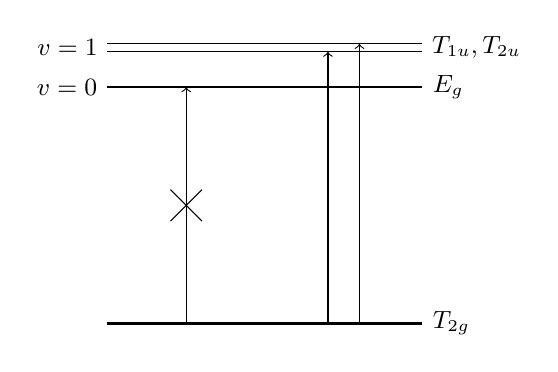
\begin{tikzpicture}
                \draw[thick] (0,0)--(4,0)node[right]{\small\(T_{2g}\)};
                \draw[thick] (0,3)node[left]{\small\(v=0\)}--(4,3)node[right]{\small\(E_g\)};
                \draw (0,3.45)--(4,3.45);
                \draw (0,3.55)--(4,3.55);
                \node at (0,3.5)[left]{\small\(v=1\)};
                \node at (4,3.5)[right]{\small\(T_{1u},T_{2u}\)};
                \draw[->] (1,0)--(1,3);
                \draw (0.8,1.7)--(1.2,1.3);
                \draw (0.8,1.3)--(1.2,1.7);
                \draw[->] (2.8,0)--(2.8,3.45);
                \draw[->] (3.2,0)--(3.2,3.55);
            \end{tikzpicture}
        \end{figure}
    \end{ex}


    \newpage
    \part*{Appendices}
    \addcontentsline{toc}{part}{\protect\numberline{}Appendices}
    \appendix

    \section{Noether's Theorem}\label{Appendix:Noether}
    The simplest way of deriving the Noether's theorem is to use the Lagrangian mechanics, which is another way of formulating classical mechanics. First let's be clear of our notations. For a system of \(N\) particles in \(d\) dimensions, we will rewrite the coordinates \(\vb{r}_i\) as \(x^A\), where \(A=1,\dots,dN\). The Newton's equations are
    \begin{equation}\label{Newtons_eqn}
        \dot{p}_A=-\pdv{V}{x^A}\,,
    \end{equation}
    where \(p_A=m_A\dot{x}^A\). To reduce the cluttering in notations, when we write \(x^A\) in the argument of a function, we mean that it is a function of all \(x^A\).
    
    Lagrangian mechanics starts from defining the Lagrangian of a system.
    \begin{defn}
        The \textit{Lagrangian} for a system is defined by
        \begin{equation}
            L(x^A,\dot{x}^A)=T(\dot{x}^A)-V(x^A)\,,
        \end{equation}
        where \(T=\frac{1}{2}\sum_{A}m_A(\dot{x}^A)^2\) is the kinetic energy and \(V(x^A)\) is the potential energy.
    \end{defn}
    Note the weird minus sign between the kinetic and the potential energy. Despite this strange definition of the Lagrangian, it works really elegantly.

    If we know that at \(t=t_0\), the particles are at \(x^A(t_0)=x^A_0\), and at \(t=t_1\), the particles are at \(x^A(t_1)=x^A_1\), there are infinite ways the systems can evolve with times between these two end points. How do we find the true paths \(x^A(t)\) taken by the particles?
    \begin{thm}[Principle of Least Action]
        The actual path taken by the system is an extremum of the \textit{action}, defined by
        \begin{equation}
            S[x^A(t)]=\int_{t_0}^{t_1}\dd{t}L(x^A(t),\dot{x}^A(t))\,.
        \end{equation}
    \end{thm}
    The \(S\) is an example of a \textit{functional}. It maps functions to a number.
    \begin{proof}
        Consider varying a given path slightly, so
        \begin{equation}
            x^A(t)\longrightarrow x^A(t)+\delta x^A(t)\,,
        \end{equation}
        where we fix the end points of the path by demanding \(\delta x^A(t_0)=\delta x^A(t_1)=0\). Then this results in a change in the action
        \begin{align}
            \delta S&=\delta\left[\int_{t_0}^{t_1}\dd{t}L\right]\notag\\
            &=\int_{t_0}^{t_1}\dd{t}\delta L\notag\\
            &=\int_{t_0}^{t_1}\dd{t}\sum_{A}\pdv{L}{x^A}\delta x^A+\pdv{L}{\dot{x}^A}\delta\dot{x}^A\,.
        \end{align}
        We integrate the second term by parts to get
        \begin{equation}
            \delta S=\int_{t_0}^{t_1}\dd{t}\sum_A\left[\pdv{L}{x^A}-\dv{}{t}\left(\pdv{L}{\dot{x}^A}\right)\right]\delta x^A + \left[\pdv{L}{\dot{x}^A}\delta x^A\right]_{t_0}^{t_1}\,.
        \end{equation}
        The boundary term vanishes since we required \(\delta x^A(t_0)=\delta x^A(t_1)=0\). At an extremum of the action \(S\), \(\delta S=0\) for all changes in the path \(\delta x^A(t)\). This holds if and only if
        \begin{equation}\label{Euler_Lagrange}
            \pdv{L}{x^A}-\dv{}{t}\left(\pdv{L}{\dot{x}^A}\right)=0\,.
        \end{equation}
        for all \(A\). These are known as the Euler--Lagrange equations. To finish the proof, we only need to show that Euler--Lagrange equations are equivalent to Newton's equations. From the definition of the Lagrangian, we have
        \begin{equation}
            \pdv{L}{x^A}=-\pdv{V}{x^A}\,,
        \end{equation}
        while
        \begin{equation}
            \pdv{L}{\dot{x}^A}=p_A\,.
        \end{equation}
        Then it's easy to see that Newton's equations (\ref{Newtons_eqn}) are indeed equivalent to Euler--Lagrange equations (\ref{Euler_Lagrange}).\qed
    \end{proof}

    In fact Lagrangian mechanics is much more powerful than that. It turns out we can use any generalised coordinate we want (e.g. spherical, hyperbolic, or just some arbitrary parameters that uniquely defines the configuration of the system), and we may add constraints to the coordinates, making it much more powerful than Newton's formulation of classical mechanics. Unfortunately, we can't go into too much detail here. If you are interested, see e.g. Prof. David Tong's notes on \href{https://www.damtp.cam.ac.uk/user/tong/dynamics.html}{Classical Dynamics}. But the important conclusion is that for any Lagrangian written in generalised coordinates \(L(q_i,\dot{q}_i,t)\), the Euler--Lagrange equations still hold:
    \begin{equation}
        \pdv{L}{q_i}-\dv{}{t}\left(\pdv{L}{\dot{q}_i}\right)=0\,.
    \end{equation}

    \begin{defn}
        Consider a one-parameter transformation of maps
        \begin{equation}
            q_i(t)\longrightarrow Q_i(s,t)
        \end{equation}
        for \(s\in\RR\) such that \(Q_i(0,t)=q_i(t)\). Then this transformation is said to be a \textit{continuous symmetry} of the Lagrangian \(L\) if
        \begin{equation}
            \pdv{}{s}L(Q_i(s,t),\dot{Q}_i(s,t),t)=0\,.
        \end{equation}
    \end{defn}
    \begin{thm}[Noether's theorem]
        For each continuous symmetry, there is a conserved quantity.
    \end{thm}
    \begin{proof}
        \begin{equation}
            \pdv{L}{s}=\sum_i \pdv{L}{Q_i}\pdv{Q_i}{s}+\pdv{L}{\dot{Q}_i}\pdv{\dot{Q}_i}{s}\,,
        \end{equation}
        so we have
        \begin{align}
            0=\pdv{L}{s}\bigg|_{s=0}&=\sum_i\pdv{L}{q_i}\pdv{Q_i}{s}\bigg|_{s=0}+\pdv{L}{\dot{q}_i}\pdv{\dot{Q}_i}{s}\bigg|_{s=0}\notag\\
            &=\sum_i\dv{}{t}\left(\pdv{L}{\dot{q}_i}\right)\pdv{Q_i}{s}\bigg|_{s=0}+\pdv{L}{\dot{q}_i}\pdv{\dot{Q}_i}{s}\bigg|_{s=0}\notag \\
            &=\dv{}{t}\left(\sum_i\pdv{L}{\dot{q}_i}\pdv{Q_i}{s}\bigg|_{s=0}\right)\,.
        \end{align}
        The quantity
        \begin{equation}
            \sum_i\pdv{L}{\dot{q}_i}\pdv{Q_i}{s}\bigg|_{s=0}
        \end{equation}
        is constant for all time.\qed
    \end{proof}

    Let's find some examples.
    \begin{ex}
        \textit{Homogeneity of space}.

        Consider a system of \(N\) particles with Lagrangian
        \begin{equation}
            L=\frac{1}{2}\sum_i m_i\dot{\vb{r}_i}^2-V(r_{ij})\,,
        \end{equation}
        where \(V(r_{ij})\) means that the potential is only dependent on the relative distances \(r_{ij}=\norm{\vb{r}_i-\vb{r}_j}\) between particles, not on their absolute positions. Then this Lagrangian has symmetry of translation: \(\vb{r}_i\to\vb{r}_i+s\vb{n}\) for any vector \(\vb{n}\) and real number \(s\).
        \begin{equation}
            L(\vb{r}_i,\dot{\vb{r}}_i,t)=L(\vb{r}_i+s\vb{n},\dot{\vb{r}}_i,t)\,.
        \end{equation}
        Then by Noether's theorem, the constant that holds in constant is
        \begin{equation}
            \sum_i\pdv{L}{\dot{\vb{r}}_i}\vdot\vb{n}=\sum_i\vb{p}_i\vdot\vb{n}\,.
        \end{equation}
        The component of linear momentum in any direction is conserved, and hence
        \begin{equation}
            \sum_i\vb{p}_i
        \end{equation}
        is also conserved.

        Homogeneity in space \(\implies\) translational invariance of \(L\) \(\implies\) conservation of total linear momentum.
    \end{ex}
    \begin{ex}
        \textit{Isotropy of Space}.

        The isotropy of space means that a closed system is invariant under rotations around an axis \(\vu{n}\), so all \(\vb{r}_i\to\vb{r}_i'\) are rotated by the same amount. To work out the corresponding conserved quantity it suffices to work with the infinitesimal form of the rotations
        \begin{equation}
            \vb{r}_i\longrightarrow \vb{r}_i+\delta\vb{r}_i=\vb{r}_i+\alpha\vu{n}\cross\vb{r}_i\,,
        \end{equation}
        where \(\alpha\) is infinitesimal. To see that this is indeed a rotation, you can calculate the length of the vector and notice it is preserved to linear order in \(\alpha\). Then we have
        \begin{equation}
            L(\vb{r}_i,\dot{\vb{r}}_i)=L(\vb{r}_i+\alpha\vu{n}\cross\vb{r}_i,\dot{r}_i+\alpha\vu{n}\cross\dot{\vb{r}}_i)\,,
        \end{equation}
        giving us the conserved quantity
        \begin{equation}
            \sum_i\pdv{L}{\dot{\vb{r}}_i}\vdot(\vu{n}\cross\vb{r}_i)=\sum_i\vu{n}\vdot(\vb{r}_i\cross\vb{p}_i)=\vu{n}\vdot\vb{L}\,.
        \end{equation}
        This is the component of the total angular momentum in the direction \(\vu{n}\). Since \(\vu{n}\) is arbitrary, \(\vb{L}\) is conserved.

        Isotropy of space \(\implies\) rotational invariance of \(L\) \(\implies\) conservation of total angular momentum.
    \end{ex}
    \section{Tensor Product}\label{Appendix:Tensor}
    There are many ways to define a tensor product space. The definition we will take here is a rather hands-on construction of the space, which involves picking a basis.
    \begin{defn}
        Let \(V\) and \(W\) be vector spaces over \(\mathbb{F}\) (always \(\CC\) in our cases). Let \((\vb{v}_1,\dots,\vb{v}_m)\) and \((\vb{w}_1,\dots,\vb{w}_n)\) be the bases of \(V\) and \(W\) respectively. The \textit{tensor product space} \(V\otimes W\) is an \(nm\)-dimensional vector space over \(\mathbb{F}\) with basis given by formal symbols
        \begin{equation}
            \{\vb{v}_i\otimes\vb{w}_j\mid 1\le i\le m,1\le j\le n\}
        \end{equation}
        and thus
        \begin{equation}
            V\otimes W=\left\{\sum_{i,j}\lambda_{ij}\vb{v}_i\otimes\vb{w}_j \,\middle|\, \lambda_{ij}\in\mathbb{F}\right\}
        \end{equation}
        with addition
        \begin{equation}
            \sum_{i,j}\lambda_{ij}\vb{v}_i\otimes\vb{w}_j+\sum_{i,j}\mu_{ij}\vb{v}_i\otimes\vb{w}_j=\sum_{i,j}(\lambda_{ij}+\mu_{ij})\vb{v}_i\otimes\vb{w}_j
        \end{equation}
        and inner product defined via basis
        \begin{equation}
           (\vb{v}_i\otimes\vb{w}_j)\vdot(\vb{v}_k\otimes\vb{w}_l)=(\vb{v}_i\vdot\vb{v}_k)(\vb{w}_j\vdot\vb{w}_l)\,.
        \end{equation}

        If
        \begin{equation}
            \vb{v}=\sum_i\alpha_i\vb{v}_i\in V\,,\quad\vb{w}=\sum_j\beta_j\vb{w}_j\in W\,,
        \end{equation}
        then their tensor product is defined as
        \begin{equation}
            \vb{v}\otimes\vb{w}=\sum_{i,j}\alpha_i\beta_j(\vb{v}_i\otimes\vb{w}_j)\in V\otimes W\,.
        \end{equation}
    \end{defn}

    \begin{rem}
        This allows us to compactly write a vector in a tensor product space as a matrix, with components \(\lambda_{ij}\), and hence a matrix is also known as a \textit{rank-two tensor}.
    \end{rem}

    \begin{defn}
        Let \(P:V\to V\) and \(Q:W\to W\) be linear maps (matrices) on \(V\) and \(W\) respectively. Then we define \(P\otimes Q\) to be a linear map on \(V\otimes W\), defined by
        \begin{equation}
            (P\otimes Q)(\vb{v}_i\otimes\vb{w}_j)=(P\vb{v}_i)\otimes(Q\vb{w}_j)\,.
        \end{equation}
    \end{defn}

    A direct product representation, which should really be called a \textit{tensor product representation}, is then defined as the tensor product of representations.
    \begin{defn}
        Let \(G\) be a finite group and \(\Gamma^V:G\to\GL(V)\) and \(\Gamma^W:G\to\GL(W)\) be representations of \(G\). Then the \textit{tensor product representation} \(\Gamma^V\otimes\Gamma^W\) is defined by
        \begin{align}
            \Gamma^V\otimes\Gamma^W:G&\to\GL(V\otimes W)\notag\\
            g&\mapsto\Gamma^V(g)\otimes\Gamma^W(g)\,.
        \end{align}
    \end{defn}
    \begin{prop}
        If the character of \(\Gamma^V\) is \(\chi^V\) and the character of \(\Gamma^W\) is \(\chi^W\), then the character of \(\Gamma^{V}\otimes\Gamma^{W}\) is \(\chi^V\chi^W\).
    \end{prop}
    \begin{proof}
        For \(g\in G\), let \((\vb{v}_1,\dots,\vb{v}_m)\) be a basis of \(V\) of eigenvectors of \(\Gamma^V(g)\) and let \((\vb{w}_1,\dots,\vb{w}_m)\) be a basis of eigenvectors of \(\Gamma^W(g)\), with
        \begin{equation}
            \Gamma^V(g)\vb{v}_i=\lambda_i\vb{v}_i\,,\quad\Gamma^W\vb{w}_j=\mu_j\vb{w}_j\,.
        \end{equation}
        Then
        \begin{align}
            (\Gamma^V\otimes\Gamma^W)(g)(\vb{v}_i\otimes\vb{w}_j)&=\Gamma^V(g)\vb{v}_i\otimes\Gamma^W(g)\vb{w}_j \notag\\
            &=\lambda_i\vb{v}_i\otimes\mu_j\vb{w}_j \notag\\
            &=(\lambda_i\mu_j)(\vb{v}_i\otimes\vb{w}_j)\,.
        \end{align}
        So
        \begin{equation}
            \chi^{\Gamma^V\otimes\Gamma^W}(g)=\sum_{i,j}\lambda_i\mu_j=\left(\sum_i\lambda_i\right)\left(\sum_j\mu_j\right)=\chi^{V}(g)\chi^W(g)\,.
        \end{equation}\qed
    \end{proof}

    \subsection{Symmetrised and Antisymmetrised Squares}
    Now let's work in \(\CC\) and make the two vector spaces in the tensor product to be equal, and denote
    \begin{equation}
        V^{\otimes 2}=V\otimes V\,.
    \end{equation}
    We define a permutation function
    \begin{align}
        \tau:V^{\otimes 2}&\longrightarrow V^{\otimes 2}\notag \\
        \sum\lambda_{ij}\vb{v}_i\otimes \vb{v}_j&\longmapsto \sum\lambda_{ij}\vb{v}_j\otimes \vb{v}_i\,.
    \end{align}
    This is a linear endomorphism on \(V^{\otimes 2}\) such that \(\tau^2=1\), so its eigenvalues are \(\pm 1\). We can then find its eigenspaces spanned by those eigenvectors with the same eigenvalues.
    \begin{defn}
        We define the \textit{symmetrised} and \textit{antisymmetrised (exterior) square} of \(V\) to be
        \begin{align}
            S^2V &= \{\vb{x}\in V^{\otimes 2}\mid \tau(\vb{x})=\vb{x}\}\\
            \Lambda^2 V &= \{\vb{x}\in V^{\otimes 2}\mid \tau(\vb{x})=-\vb{x}\}\,.
        \end{align}
    \end{defn}

    Then the subspace \(S^2V\) has the basis
    \begin{equation}
        \{\vb{v}_i\vb{v}_j\coloneqq \vb{v}_i\otimes\vb{v}_j+\vb{v}_j\otimes\vb{v}_i \mid 1\le i\le j\le n\}\,,
    \end{equation}
    and \(\Lambda^2V\) has the basis
    \begin{equation}
        \{\vb{v}_i\wedge\vb{v}_j\coloneqq \vb{v}_i\otimes\vb{v}_j-\vb{v}_j\otimes\vb{v}_i \mid 1\le i< j\le n\}\,.
    \end{equation}
    Hence
    \begin{equation}
        \dim S^2V=\frac{1}{2}n(n+1)\qquad\dim\Lambda^2V=\frac{1}{2}n(n-1)\,,
    \end{equation}
    and so
    \begin{equation}
        V^{\otimes 2}=S^2V\oplus\Lambda^2V\,,
    \end{equation}
    where we can write any \(\vb{x}\in V^{\otimes 2}\) as
    \begin{equation}
        \vb{x}=\underbrace{\frac{1}{2}(\vb{x}+\tau(\vb{x}))}_{\in S^2 V}+\underbrace{\frac{1}{2}(\vb{x}-\tau(\vb{x}))}_{\in \Lambda^2 V}\,.
    \end{equation}

    Those are just technical details. What we can now show is the formula of characters of symmetrised and antisymmetrised square.

    \begin{prop}
        Let \(\Gamma:G\to\GL(V)\) be a representation with character \(\chi\). Let \(\chi^S\) and \(\chi^\Lambda\) be the characters of subrepresentations of the tensor product representation \(\Gamma\otimes\Gamma\) on \(S^2V\) and \(\Lambda^2V\) respectively, then
        \begin{align}
            \chi^S(g)&=\frac{1}{2}(\chi(g)^2+\chi(g^2))\\
            \chi^\Lambda(g)&=\frac{1}{2}(\chi(g)^2-\chi(g^2))\,.
        \end{align}
    \end{prop}
    \begin{proof}
        Since \(V^{\otimes 2}=S^2V\oplus\Lambda^2V\), it is immediate that \(\chi^2=\chi^S+\chi^\Lambda\). Let \(\vb{v}_i,\dots,\vb{v}_n\) the eigenvectors of \(\Gamma(g)\) so that it is a basis of \(V\), with
        \begin{equation}
            \Gamma(g)\vb{v}_i=\lambda_i\vb{v}_i\,.
        \end{equation}
        Acting the tensor product representation on \(\Lambda^2 V\), we get
        \begin{equation}
            \Gamma\otimes\Gamma(g)(\vb{v}_i\wedge\vb{v}_j)=\lambda_i\lambda_j\vb{v}_i\wedge\vb{v}_j\,.
        \end{equation}
        Summing over all basis vectors of \(\Lambda^2 V\), we get
        \begin{equation}
            \chi^\Lambda(g)=\sum_{1\le i< j\le n}\lambda_i\lambda_j\,.
        \end{equation}
        Consider
        \begin{align}
            \chi(g)^2&=\left(\sum\lambda_i\right)^2\notag\\
            &=\sum\lambda_i^2+2\sum_{i<j}\lambda_i\lambda_j\notag\\
            &=\chi(g^2)+2\chi^\Lambda(g)\,,
        \end{align}
        and so
        \begin{equation}
            \chi^\Lambda(g)=\frac{1}{2}(\chi(g)^2-\chi(g^2))\,.
        \end{equation}
        Then
        \begin{equation}
            \chi^S=\chi^2-\chi^\Lambda=\frac{1}{2}(\chi(g)^2+\chi(g^2))\,.
        \end{equation}\qed
    \end{proof}
    This is a much more concise and elegant proof than the one presented in the main text.

    If you are interested in more of this, see e.g. Dexter Chua's notes on Mathematical Tripos Part II: \textcolor{blue}{\href{https://dec41.user.srcf.net/notes/II_L/representation_theory.pdf}{\textit{Representation Theory}}}.

\end{document}